\section{经典统计力学}
\subsection{从拉格朗日力学到相空间}
在\href{https://github.com/Astolfo-Official/Baby-Math-on-Quantum-Chemistry/blob/main/%E3%80%8A%E9%87%8F%E5%AD%90%E5%8C%96%E5%AD%A6%E4%B8%AD%E7%9A%84%E6%95%B0%E5%AD%A6%E3%80%8B2.0.pdf}{我搬运的一本速通教材的第四章}中，我们简单过了一遍经典力学。感兴趣的可以先阅读一下前置章节，这里我们会跳过许多细节直接叙述经典力学的两大形式后进入经典相空间理论的介绍。经典相空间理论也是经典力学的一种等价表述方式，但是在处理大量自由度问题也即经典统计力学中，相空间理论有其他三种形式不可比拟的优势。简单来说，在经典统计力学中，我们最后要处理的对象并不是某一条具体轨道，而是\textbf{大量可能微观状态在相空间中的分布}。这对于牛顿力学，拉格朗日力学和哈密顿力学来说都是一个全新的挑战。

在拉格朗日力学中，设体系有$3N$个广义坐标$q_i$，其运动由拉格朗日量$L(\bm{q},\dot{\bm{q}},t)=T(\bm{q},\dot{\bm{q}},t)-V(\bm{q},\dot{\bm{q}},t)$决定，其中$T$是动能，$V$是势能。对应的运动学方程即为 Euler-Lagrange 方程：
\[\dv{}{t}\left(\pdv{L}{\dot{q}_i}\right)-\pdv{L}{q_i}=0,\quad (i=1,\ldots,3N)\]
容易验证上述方程等价于牛顿第二定律。进一步地，我们还定义与广义坐标$q_i$对应的广义动量：
\[p_i=\pdv{L}{\dot{q}_i}\]
这个关系可以反解出$\dot{q}_i=\dot{q}_i(\bm{q},\bm{p},t)$，则我们可以对拉格朗日量做 Legendre 变换 [章节\ref{sec:legendre}]，进而定义哈密顿量$H(\bm{q},\bm{p},t)=\bm{p}\dot{\bm{q}}-L(\bm{q},\dot{\bm{q}},t)$。如果势能$V$与体系动量（或速度）无关，哈密顿量就是我们熟悉的总能量。把$H$看成$q_i,p_i$的函数后，对其微分并逐项比较可得哈密顿正则方程：
\[\dot{q}_i=\pdv{H}{p_i},\quad \dot{p}_i=-\pdv{H}{q_i}\]

在哈密顿形式下体系在某一时刻$t$的微观状态由全部坐标和动量唯一确定$\xi=(q_1,\ldots,q_f,p_1,\ldots,p_f)$，所有这样的点构成一个$6N$维空间，称为\textbf{相空间}；相空间中的一个点称为相点，它完整代表一个微观状态。体系随时间演化时，相点便在相空间中描出一条轨线，称为\textbf{相轨线}。如果\textcolor{blue}{\textbf{哈密顿量不显示含时间}}，则能量守恒，不同轨线被限制在各自能量面上，相空间中同一点出发的轨迹全部等同，任意交叉的轨迹都代表同一个微观状态。

至此我们把研究对象从具体的轨道转向了相空间中的分布。这时就可以引入统计的概念：对同一个宏观系统，在给定时刻所有可能微观状态组成一个系综；若记相空间概率密度为$\rho(\bm{q},\bm{p},t)$，则满足归一化：
\[\int\rho(\bm{q},\bm{p},t)\dd\bm{\Gamma}=\frac{1}{h^{3N}}\int\rho(\bm{q},\bm{p},t)\dd^{3N}\bm{q}\dd^{3N}\bm{p}=1\]
这里$h$是相空间微分$\dd{\bm{\Gamma}}$的体积，一般取为 Planck 常数。于是任意可观测量$F(\bm{p},\bm{q},t)$的系综平均都可写为：
\[\langle F \rangle=\int F(\bm{p},\bm{q},t)\rho(\bm{q},\bm{p},t)\dd{\bm{\Gamma}}\]
考虑对$F$求对时间$t$的全导数并带入哈密顿正则方程：
\[\dv{F}{t}=\pdv{F}{t}+\sum_i\left(\pdv{F}{q_i}\dot{q}_i+\pdv{F}{p_i}\dot{p}_i\right)=\pdv{F}{t}+\sum_i\left(\pdv{F}{q_i}\pdv{H}{p_i}-\pdv{F}{p_i}\pdv{H}{q_i}\right)=\pdv{F}{t}+\{F,H\}\]
其中 Poisson 括号定义为：
\[\{F,G\}=\sum_i\left(\pdv{F}{q_i}\pdv{G}{p_i}-\pdv{F}{p_i}\pdv{G}{q_i}\right)\]
另一方面，概率守恒要求概率密度$\rho(\bm{q},\bm{p},t)$满足连续性方程：
\[\begin{aligned}
\pdv{\rho}{t}+\nabla\cdot(\rho \dot{\xi})&=\pdv{\rho}{t}+\nabla\rho\cdot\dot{\xi}+\rho(\nabla\cdot\dot{\xi})=\pdv{\rho}{t}+\nabla\rho\cdot\dot{\xi}+\rho\sum_{i=1}^{f}\left(\pdv{\dot{q}_i}{q_i}+\pdv{\dot{p}_i}{p_i}\right)\\
&=\pdv{\rho}{t}+\nabla\rho\cdot\dot{\xi}+\rho\sum_{i=1}^{f}\left(\pdv{}{q_i}\pdv{H}{p_i}-\pdv{}{p_i}\pdv{H}{q_i}\right)=\pdv{\rho}{t}+\nabla\rho\cdot\dot{\xi}=0 \quad \Leftrightarrow \quad \dv{\rho}{t}=0
\end{aligned}\]
这就是 Liouville 方程。它告诉我们：\textcolor{blue}{\textbf{在精确的哈密顿演化下，相空间中的概率流像不可压缩流体一样运动}}，局部概率密度沿着相轨线保持不变。若哈密顿量不显含时间，则能量守恒，相点始终停留在某个能量面，记为$\Gamma_E:\ H(\bm{q},\bm{p})=E$，在 Liouville 方程的约束下，轨迹的运动可以与流类比，我们考虑两种流：
\begin{itemize}
\item 1. 非遍历性流（Non-ergodic）：轨线在能量面上只占据一个子区域，如周期性运动；
\item 2. 遍历性流（Ergodic）：轨线在能量面上占据整个区域。
\end{itemize}
如果体系的流是遍历的，那么一条足够长的轨线在长时间平均意义下就能代表整个能量面的平均，即：
\[\overline{f}=\lim_{T\to\infty}\frac{1}{T}\int_0^T f(\bm{q},\bm{p})\dd t=\frac{1}{\Sigma_E}\int f(\bm{q},\bm{p})\delta(H(\bm{q},\bm{p})-E)\dd{\bm{\Gamma}}=\langle f \rangle_E\]
此时可定义能量面截面（微正则配分函数）与微正则分布：
\[\Sigma_E=\int\delta(H(\bm{q},\bm{p})-E)\dd{\bm{\Gamma}}, \quad \rho_E(\bm{q},\bm{p})=\frac{1}{\Sigma_E}\delta(H(\bm{q},\bm{p})-E)\]
可以看出在给定能量时，能量面上每个可及微观状态都被赋予相同权重。再考虑\textbf{混合流}，一种特殊的遍历流，\textcolor{blue}{\textbf{从任意时刻$t$的（非平衡）分布$\rho(\bm{q},\bm{p},t)$开始演化，经过足够长的时间后，系统的分布都会演化成微正则分布}}：
\[\lim_{t\to\infty}\rho(\bm{q},\bm{p},t)=\rho_E(\bm{q},\bm{p})\]
刘维尔定理（体积元守恒）与混合效应相结合表明：相空间中的无穷小体积元会经历无限的拉伸与折叠，并最终弥散分布于整个能量曲面上。因此\textcolor{blue}{\textbf{微观分布与初始状态无关}}，这就是经典统计力学的核心假设之一。\textcolor{blue}{\textbf{微观分布一旦确定，宏观量都可以视为相空间的期望值}}。

\subsection{微正则系综}
上一小节我们介绍了微正则系综，并给出了微正则配分函数$\Sigma_E$和微正则分布$\rho_E$的定义。显然我们可以知道在微正则系综中系统粒子数$N$和能量$E$是固定的。我们再来考虑体积$V$，如果体积$V$是可变的那么，会导致哈密顿量的势能显含时间，不满足微正则系综的条件，因此微正则系综的控制变量是$(N,V,E)$。因此微正则系综既不与外界交换热，也不交换粒子，所有满足给定能量壳层的微观状态被赋予等概率。记微正则配分函数为：
\[\Omega(N,V,E)=\int\delta(H(\bm{q},\bm{p})-E)\dd{\bm{\Gamma}}\]
$\Omega(N,V,E)$可以认为是体系的微观状态数，微正则系综中每个可及状态的概率都等于$1/\Omega$，Boltzmann 熵定义为：
\[S(N,V,E)=k_{\rm B}\ln \Omega(N,V,E)\]
上述 Boltzmann 熵可以认为是 Gibbs 熵在微正则系综中（等概率情况）的特殊情况，从 Gibbs 熵的定义出发：
\[S=-k_{\rm B}\int\rho(\bm{q},\bm{p})\ln\rho(\bm{q},\bm{p})\dd{\bm{\Gamma}}\]
其中密度分布函数$\rho(\bm{q},\bm{p})$可以认为在一个极小能量壳层$(\bm{q},\bm{p})\in \Gamma_{E}$内均匀分布：
\[\rho(\bm{q},\bm{p})=\frac{1}{\Omega(N,V,E)} \quad \Rightarrow \quad 
S=-k_{\rm B}\int_{\Gamma_{E}}\frac{1}{\Omega}\ln\frac{1}{\Omega}\dd{\bm{\Gamma}}=-k_{\rm B}\frac{1}{\Omega}\ln\frac{1}{\Omega}\int_{\Gamma_{E}}\dd{\bm{\Gamma}}=-k_{\rm B}\frac{1}{\Omega}\ln\frac{1}{\Omega}\cdot \Omega=k_{\rm B}\ln\Omega\]
同时我们也可以证明当 Gibbs 熵对分布函数做变分，在满足归一化约束的条件下达到极大值时，分布函数必然是微正则分布$\rho_E$，此时 Gibbs 熵就退化成 Boltzmann 熵。考虑对以下函数做变分：
\[\mathcal{S}=-k_{\rm B}\int\rho(\bm{q},\bm{p})\ln\rho(\bm{q},\bm{p})\dd{\bm{\Gamma}}-\lambda\left(\int\rho(\bm{q},\bm{p})\dd{\bm{\Gamma}}-1\right) \quad \Rightarrow \quad \delta\mathcal{S}=-k_{\rm B}\int\delta\rho(\bm{q},\bm{p})\left[\ln\rho(\bm{q},\bm{p})+1-\lambda\right]\dd{\bm{\Gamma}}=0\]
因此要求$\rho(\bm{q},\bm{p})$为常数，带入归一化条件：
\[\int \rho(\bm{q},\bm{p}) \dd{\bm{\Gamma}} = \rho(\bm{q},\bm{p})\int \dd{\bm{\Gamma}} = \rho(\bm{q},\bm{p})\Omega(N,V,E) = 1 \quad \Leftrightarrow \quad \rho(\bm{q},\bm{p}) = \frac{1}{\Omega(N,V,E)}\]
此时，在对$\mathcal{S}$做二阶变分：
\[\delta^2\mathcal{S}=-k_{\rm B}\int\frac{1}{2}\delta^2\rho(\bm{q},\bm{p})\cdot\frac{1}{\rho(\bm{q},\bm{p})}\dd{\bm{\Gamma}}<0\]
即😄$\mathcal{S}$在微正则分布处取得极大值。此外如果系统的密度分布满足$\rho=\rho_1\rho_2$，则\textcolor{blue}{\textbf{体系的熵$S$满足可加性}}：
\[S=-k_{\rm B}\int\rho\ln\rho\dd{\bm{\Gamma}}=-k_{\rm B}\left(\int\rho_1\ln\rho_1\dd{\bm{\Gamma}_1}\cdot\int\rho_2\dd{\bm{\Gamma}_2}+\int\rho_2\ln\rho_2\dd{\bm{\Gamma}_2}\cdot\int\rho_1\dd{\bm{\Gamma}_1}\right)=S_1+S_2\]

对 Boltzmann 熵做全微分：
\[\dd S=k_{\rm B}\left(\pdv{\ln\Omega}{N}\right)_{V,E}\dd N+k_{\rm B}\left(\pdv{\ln\Omega}{V}\right)_{N,E}\dd V+k_{\rm B}\left(\pdv{\ln\Omega}{E}\right)_{N,V}\dd E\]
另一方面，由热力学基本关系：
\[\dd U=T\dd S-P\dd V+\mu \dd N \quad \Rightarrow \quad \dd S=\frac{1}{T}\dd U+\frac{P}{T}\dd V-\frac{\mu}{T}\dd N\]
在微正则系综里$U=E$，逐项比较便得到：
\begin{equation}\label{eq:nve_terms}
\frac{1}{T}=k_{\rm B}\left(\pdv{\ln\Omega}{E}\right)_{N,V}, \quad P=k_{\rm B} T\left(\pdv{\ln\Omega}{V}\right)_{N,E}, \quad \mu=-k_{\rm B} T\left(\pdv{\ln\Omega}{N}\right)_{V,E}
\end{equation}
一旦$T,P,\mu$被确定，其余常见热力学势都可以通过 Legendre 变换得到：
\begin{equation}\label{eq:Legendre_4}
\boxed{U=E,\quad F=U-TS=E-k_{\rm B} T\ln\Omega, \quad H=U+PV=E+PV, \quad G=F+PV=U+PV-TS}
\end{equation}
对于可加的均匀体系，Euler 关系还给出$G=\sum_i\mu_i N_i$，其中$i$指代不同种类的粒子。
\begin{proposition}[微正则系综下的单原子理想气体]
在体积$V$的盒子中的$N$个单原子理想气体，体系哈密顿量满足：
\[H=\sum_{i=1}^{N}\frac{\bm{p}_i^2}{2m}=E\]
\end{proposition}
按照定义，容易看出微正则配分函数为：
\[\widetilde{\Omega}(N,V,E)=\frac{1}{h^{3N}}\int \delta\!\left(\sum_{i=1}^{N}\frac{\bm{p}_i^2}{2m}-E\right)\dd^{3N}\bm{q}\,\dd^{3N}\bm{p}=\frac{V^N}{h^{3N}}\int \delta\!\left(\frac{\bm{p}^2}{2m}-E\right)\dd^{3N}\bm{p}\equiv \frac{V^N}{h^{3N}}I\]
上式中的动量积分可以实际上是$3N$维空间中对一个半径为$\sqrt{2mE}$的超球面进行积分。利用$\delta$函数的性质：
\[\delta\!\left(\frac{p^2}{2m}-E\right)=\frac{\delta(p-\sqrt{2mE})}{|f'(\sqrt{2mE})|}=\sqrt{\frac{m}{2E}}\delta(p-\sqrt{2mE})\]
这个超球面的面积为：
\[\begin{aligned}
I&=\int\delta\!\left(\frac{p^2}{2m}-E\right)p^{3N-1}\dd p\dd{\bm{\Gamma}_{3N-1}}=\frac{2\pi^{3N/2}}{\Gamma(3N/2)}\int_0^\infty p^{3N-1}\delta\!\left(\frac{p^2}{2m}-E\right)\dd p\\
&=\frac{2\pi^{3N/2}}{\Gamma(3N/2)}\sqrt{\frac{m}{2E}}\int_0^\infty p^{3N-1}\delta(p-\sqrt{2mE})\dd p=\frac{2\pi^{3N/2}}{\Gamma(3N/2)}\sqrt{\frac{m}{2E}}\sqrt{2mE}^{3N-1}=\frac{(2\pi m)^{3N/2}}{\Gamma(3N/2)}E^{3N/2-1}
\end{aligned}\]
从而：
\[\widetilde{\Omega}(N,V,E)=\frac{V^N}{h^{3N}}\frac{(2\pi m)^{3N/2}}{\Gamma(3N/2)}E^{3N/2-1}\]
利用 Stirling 公式$\ln\Gamma(n)\sim n\ln n-n$，对应的微正则熵为：
\[\widetilde{S}(N,V,E)=k_{\rm B}\ln \widetilde{\Omega}(N,V,E)\sim Nk_{\rm B}\left\{\ln\left[V\left(\frac{4\pi mE}{3Nh^2}\right)^{3/2}\right]+\frac{3}{2}\right\}\]
进而可以求解其他热力学函数，首先是温度$T$和压强$P$：
\[\frac{1}{T}=\left(\pdv{\widetilde{S}}{E}\right)_{N,V}\sim\frac{3Nk_{\rm B}}{2E}, \quad P=T\left(\pdv{\widetilde{S}}{V}\right)_{N,E}=\frac{Nk_{\rm B} T}{V}\]
稍微改写一下就可以获得单原子理想气体能量$U=E=3Nk_{\rm B} T/2$以及状态方程$PV=Nk_{\rm B}T$。计算化学势：
\[\widetilde{\mu}=-T\left(\pdv{\widetilde{S}}{N}\right)_{V,E}=-k_{\rm B} T\ln\left[V\left(\frac{4\pi mE}{3Nh^2}\right)^{3/2}\right]\]
这个结果已经暴露出问题：\textcolor{blue}{\textbf{化学势本应是强度量，但这里它直接依赖于总体积$V$而不是粒子密度$N/V$}}。更严重的问题是熵不再是广延量：考虑两份完全相同的同种理想气体，各自处于$(N,V,E)$。抽去隔板前总熵为$2\widetilde{S}(N,V,E)$，抽去隔板后若仍把粒子当成可分辨粒子来数，则$\widetilde{S}_{\rm after}=2\widetilde{S}(N,V,E)+2Nk_{\rm B}\ln 2$，\textcolor{blue}{\textbf{但这显然不合理，因为两边本来就是同一种气体、相同温度、相同密度，抽去隔板并没有产生新的可观测宏观状态，熵增理应为零}}。

上述问题也被称为\textbf{ Gibbs 悖论}。在20世纪初期 Gibbs 本人提出了一个备受争议的解决方案：如果两个完全相同的相交换粒子不改变围观状态，因此在围观状态数中引入了因子$1/N!$以消除过度计数问题：
\begin{equation}\label{eq:partition_nve_mono}
\Omega(N,V,E)=\frac{\widetilde{\Omega}(N,V,E)}{N!}=\frac{V^N}{N!h^{3N}}\frac{(2\pi m)^{3N/2}}{\Gamma(3N/2)}E^{3N/2-1}
\end{equation}
1911 年到 1916 年，Sackur、Tetrode、Planck 更进一步，将上述 Gibbs 提出的修正过的围观状态数应用于熵与化学式熵，解决了熵无法广延 [Sackur-Tetrode 公式] 和化学势不是强度量的问题：
\[\begin{aligned}
S(N,V,E) &=Nk_{\rm B}\left\{\ln\left[\frac{V}{N}\left(\frac{4\pi mE}{3Nh^2}\right)^{3/2}\right]+\frac{5}{2}\right\}\\
\mu(N,V,E)&=-k_{\rm B} T\ln\left[\frac{V}{N}\left(\frac{4\pi mE}{3Nh^2}\right)^{3/2}\right]
\end{aligned}\]
但这在当时并没有被所有人接受。1921 年 Ehrenfest 和 Trkal 还批评说：在经典力学里粒子原则上可以靠轨迹区分，所以$1/N!$并不是由经典动力学“强迫”出来的，而更像是为了让统计热力学与经验热力学一致而加上的规则。

但不管怎么说我们最终获得了正确的微正则配分函数，由它再来计算与粒子数相关的热力学量，就会得到完全正确且具有正常标度性质的结果。我们把单原子理想气体能量$U=E=3Nk_{\rm B} T/2$带入上述熵和化学式中对数函数中的那一大坨：
\[\frac{4\pi mE}{3Nh^2}=\frac{4\pi m}{3h^2}\left(\frac{3Nk_{\rm B} T}{2}\right)=\frac{2\pi m k_{\rm B} T}{h^2} \quad \Rightarrow \quad \Lambda=\frac{h}{\sqrt{2\pi mk_{\rm B}T}}\]
通过上述方式定义出来的$\Lambda$被称为\textbf{热波长}，它是一个长度量纲的物理量，代表了粒子热运动的空间尺度。之后我们会经常见到它。\textcolor{blue}{\textbf{记住，在微正则系综可以作为变量的函数只有N，V和E，因此即使上述热波长引入了温度也不要把温度作为变量去运算，正确的做法应该是以N，V和E作为变量运算后再最后带入热波长进行化简！！！}}最后汇总一下微正则系综下单原子理想气体的热力学函数，记粒子数密度$n=N/V$：
\begin{theorem}[微正则系综下单原子理想气体的热力学函数]
\[\Omega(N,V,E)=\frac{V^N}{N!h^{3N}}\frac{(2\pi m)^{3N/2}}{\Gamma(3N/2)}E^{3N/2-1}, \quad S(N,V,E) \sim Nk_{\rm B}\left[\frac{5}{2}-\ln(n\Lambda^3)\right]\]
\[\left\{\begin{aligned}
U&=E=\frac{3}{2}Nk_{\rm B} T\\
F&=U-TS=-Nk_{\rm B} T\left[-\ln\left(n\Lambda^3\right)+1\right]\\
H&=U+PV=\frac{5}{2}Nk_{\rm B} T\\
G&=F+PV=\mu N=Nk_{\rm B} T\ln(n\Lambda^3)\\
\end{aligned}\right.
\quad \Rightarrow \quad
\left\{\begin{aligned}
PV&=Nk_{\rm B} T\\
C_V&=\left(\pdv{U}{T}\right)_{V,N}=\frac{3}{2}Nk_{\rm B}\\
C_P&=\left(\pdv{H}{T}\right)_{P,N}=\frac{5}{2}Nk_{\rm B}\\
\mu&=k_{\rm B} T\ln(n\Lambda^3)
\end{aligned}\right.\]
\end{theorem}

最后的最后我们以马后炮角度来看看 Gibbs 悖论的解决方案。作为一个21世纪的学过量子力学的人我们知道$1/N!$的引入是由于\textcolor{blue}{\textbf{微观粒子的全同性}}的必然要求。Gibbs 在一个还没有量子力学的时代敢提出这个解决方案也是非常的超前。但我们也要注意到，量子力学的全同性原则是一个后续发展出来的理论，而不是从经典力学中直接推导出来的，因此在经典力学框架下，$1/N!$的引入确实是一个人为的修正。

但是话说回来，原先在经典统计中定义的相空间微元：
\[\dd{\bm{\Gamma}}=\frac{\dd{^{3N}\bm{p}}\dd{^{3N}\bm{q}}}{h^{3N}}\]
在经典框架内也并不意味着有问题。比如在很多教材中会出现的\textbf{经典定域子系统}，如果考虑经典粒子的话上述定义是完全合理的。但是当我们把统计的边界逐渐推向微观世界时，经典理论的框架就会逐渐失效。其实把相点的体积取为 Planck 常数也是为了让经典统计力学的结果与量子统计力学的结果在热力学极限下保持一致而引入的一个修正。这也是在经典框架下迫近微观量子世界时不得不做的妥协。

\newpage
\subsection{正则系综与玻尔兹曼分布}
从时间上来说，人类对统计力学的研究始于 Boltzmann 对微正则系综（孤立系统）中能量交换的研究，因此我们也将以 Boltzmann 分布的推导作开始本小节正则系综的介绍。考虑一个小系统$A$与一个巨大热浴$B$接触，二者组成的总体系孤立，总能量固定为$E_{\rm tot}$，是一个微正则系综。若系统$A$处于能量本征值$E_i$对应的微观状态，则热浴的能量就是$E_{\rm tot}-E_i$，于是该状态出现的概率正比于热浴在该能量下的微观态数：
\[P_i\propto \Omega_B(E_{\rm tot}-E_i)\]
给定体系能量后热浴$B$的能量也确定，因此也是微正则系综，对热浴态数在$E_{\rm tot}$附近做 Taylor 展开：
\[\ln \Omega_B(E_{\rm tot}-E_i)=\ln \Omega_B(E_{\rm tot})-\left(\pdv{\ln\Omega_B}{E_B}\right)_{V,N}E_i+\cdots \quad \Rightarrow \quad \left(\pdv{\ln\Omega_B}{E_B}\right)_{V,N}=\frac{1}{k_{\rm B}}\left(\pdv{S_B}{E_B}\right)_{V,N}=\frac{1}{k_{\rm B} T}\]
进而可知系统$A$处于能量$E_i$的概率（简并度为$g_i$）以及归一化因子$Z$为：
\[P_i=\frac{g_i}{Z}\exp\left(-\frac{E_i}{k_{\rm B} T}\right)\equiv\frac{g_i}{Z}e^{-\beta E_i}, \quad Z=\sum_i g_i\exp\left(-\frac{E_i}{k_{\rm B} T}\right)\equiv\sum_i g_i e^{-\beta E_i}\]
Boltzmann 研究的系统能与热浴交换能量、但体积$V$和粒子数$N$都固定，其全部微观状态按这一权重组成的统计集合就称为\textcolor{blue}{\textbf{正则系综}}。因此正则系综的自然变量是$(N,V,T)$。在经典相空间表述下，玻尔兹曼分布可以写成：
\[\rho(\xi)=\frac{e^{-\beta H(\xi)}}{Z(N,V,T)},\quad Z(N,V,T)=\int e^{-\beta H(\xi)}\dd\bm{\Gamma}\]
从 Gibbs 熵定义出发，带入正则分布可以获得熵关于正则配分函数的表达式：
\[S=-k_{\rm B}\int \rho(\xi)\ln\rho(\xi)\dd\Gamma=k_{\rm B}\beta\int \rho(\xi)H(\xi)\dd\Gamma+k_{\rm B}\ln Z(N,V,T)\int \rho(\xi)\dd\Gamma=k_{\rm B}\beta U+k_{\rm B}\ln Z(N,V,T)\]

从微正则系综的角度回看正则系综，还能得到一个很有启发的结果。若把总概率改写成能量的分布，则：
\begin{equation}\label{eq:eqnvt}
p(E)=\frac{\Omega(N,V,E)e^{-\beta E}}{Z(N,V,T)}=\frac{1}{Z(N,V,T)}\exp\left[\frac{S(N,V,E)}{k_{\rm B}}-\beta E\right]=\frac{1}{Z(N,V,T)}e^{-\beta F(N,V,E)}
\end{equation}
因此最概然能量对应的其实就是$F(N,V,E)$的极小值点，这也解释了为什么\textcolor{blue}{\textbf{ Helmholtz 自由能会成为正则系综的核心热力学势}}。由定义（callback 一下$\xi=(\bm{p},\bm{q})$是相点）出发推导其他热力学函数，如内能：
\[U=\int H(\xi)\rho(\xi)\dd\Gamma=\frac{1}{Z}\int H(\xi)e^{-\beta H(\xi)}\dd\Gamma=-\frac{1}{Z}\pdv{Z}{\beta}=-\pdv{\ln Z}{\beta}\]
再利用$F=U-TS$，得到 Helmholtz 自由能$F=U-T\left[k_{\rm B}\beta U+k_{\rm B}\ln Z\right]=-k_{\rm B}T\ln Z$。考虑$F$的全微分$\dd F=-S\dd T-P\dd V+\mu \dd N$可以得到压强$P$和化学势$\mu$，以及其他热力学函数如下：
\begin{theorem}[正则系综的基本热力学关系]
\[\rho(\xi)=\frac{e^{-\beta H(\xi)}}{Z},\quad Z=\int e^{-\beta H(\xi)}\dd\Gamma, \quad S=k_{\rm B}\left(\ln Z+\beta U\right)\]
\[\left\{\begin{aligned}
U&=-\pdv{\ln Z}{\beta}\\
F&=-k_{\rm B} T\ln Z\\
H&=-\pdv{\ln Z}{\beta}+k_{\rm B}TV\left(\pdv{\ln Z}{V}\right)_{N,T}\\
G&=-k_{\rm B} T\ln Z+k_{\rm B}TV\left(\pdv{\ln Z}{V}\right)_{N,T}
\end{aligned}\right.
\quad \Rightarrow \quad
\left\{\begin{aligned}
P&=k_{\rm B} T\left(\pdv{\ln Z}{V}\right)_{N,T}\\
\mu&=-k_{\rm B} T\left(\pdv{\ln Z}{N}\right)_{V,T}\\
C_V&=\left(\pdv{U}{T}\right)_{N,V}=k_{\rm B}\beta^2\pdv[2]{\ln Z}{\beta}\\
\expval{(\Delta E)^2}&=\pdv[2]{\ln Z}{\beta}=k_{\rm B} T^2 C_V
\end{aligned}\right.\]
\end{theorem}
如果体系满足通常的可加性关系，则依然有$G=\mu N$。正则系综里一个非常重要的结果是能量涨落公式：
\[\expval{(\Delta E)^2}=\expval{H^2}-\expval{H}^2=\frac{1}{Z}\pdv[2]{Z}{\beta}-\frac{1}{Z^2}\left(\pdv{Z}{\beta}\right)^2=\pdv{\beta}\left(\frac{1}{Z}\pdv{Z}{\beta}\right)=\pdv[2]{\ln Z}{\beta}=k_{\rm B} T^2 C_V\]
因此热容不仅描述“升温有多难”，也直接控制平衡能量涨落的大小。下面我们来看两个具体例子。

\begin{proposition}[正则系综下的单原子理想气体]
在在温度$T$，体积$V$的盒子中的$N$个单原子理想气体，体系哈密顿量由动能给出：
\[H=\sum_{i=1}^{N}\frac{\bm{p}_i^2}{2m}=\sum_{i=1}^{N}\frac{1}{2}m\bm{v}_i^2=\frac{1}{2}m\bm{v}^2, \quad \bm{v}^2=\sum_{i=1}^{N}\bm{v}_i^2\]
\end{proposition}
对单个理想气体粒子而言，玻尔兹曼权重直接给出三维速度分布，积分掉角度部分，另$v=|\bm{v}|$，则：
\[f(\bm{v})=\left(\frac{m}{2\pi k_{\rm B} T}\right)^{3/2}\exp\left(-\frac{m\bm{v}^2}{2k_{\rm B} T}\right) \quad \Rightarrow \quad f(v)=4\pi \left(\frac{m}{2\pi k_{\rm B} T}\right)^{3/2}v^2\exp\left(-\frac{mv^2}{2k_{\rm B} T}\right)\]
把变量从$v$换成$\varepsilon=mv^2/2$，由概率守恒$f(\varepsilon)\dd\varepsilon=f(v)\dd v$可得单粒子平动能量分布：
\[f(\varepsilon)
=f(v)\left|\dv{v}{\varepsilon}\right|=4\pi \left(\frac{m}{2\pi k_{\rm B} T}\right)^{3/2}\left(\frac{2\varepsilon}{m}\right)\exp\left(-\frac{\varepsilon}{k_{\rm B} T}\right)\frac{1}{\sqrt{2m\varepsilon}}=\frac{2}{\sqrt{\pi}} \frac{\sqrt{\varepsilon}}{(k_{\rm B} T)^{3/2}}e^{-\varepsilon/(k_{\rm B} T)}\]
最概然能量由$f(\varepsilon)$的极大值条件决定。对$\ln f(\varepsilon)$求导更方便：
\[
\dv{}{\varepsilon}\ln f(\varepsilon)=\frac{1}{2\varepsilon}-\frac{1}{k_{\rm B} T}=0
\quad \Rightarrow \quad
\varepsilon_{\rm mp}=\frac{1}{2}k_{\rm B} T.
\]
更一般地，令$x=\varepsilon/(k_{\rm B}T)$，则任意矩都可以写成 Gamma 函数积分：
\[\expval{\varepsilon^n}=\int_0^\infty \varepsilon^n f(\varepsilon)\dd\varepsilon=\frac{2}{\sqrt{\pi}}(k_{\rm B} T)^n\int_0^\infty x^{n+1/2}e^{-x}\dd x=\frac{2}{\sqrt{\pi}}\Gamma\left(n+\frac{3}{2}\right)(k_{\rm B} T)^n\]
取$n=1,2$便得到平均能量$\expval{\varepsilon}$和平均平方能量$\expval{\varepsilon^2}$，以及能量涨落$\expval{(\Delta \varepsilon)^2}$：
\[\boxed{\expval{\varepsilon}=\frac{3}{2}k_{\rm B} T,\quad \expval{\varepsilon^2}=\frac{15}{4}(k_{\rm B} T)^2,\quad \expval{(\Delta \varepsilon)^2}=\expval{\varepsilon^2}-\expval{\varepsilon}^2=\frac{3}{2}(k_{\rm B} T)^2}\]

上式给出的是\textbf{单粒子}能量$\varepsilon$的统计性质。由于理想气体粒子没有相互作用，所以在正则系综中$\varepsilon_1,\cdots,\varepsilon_N$彼此独立同分布，并且都服从上面的$f(\varepsilon)$。因此总能量的平均值可以直接由单粒子平均能量相加得到：
\[E=\sum_{i=1}^{N}\varepsilon_i \quad \Rightarrow \quad\expval{E}=\sum_{i=1}^{N}\expval{\varepsilon_i}=N\expval{\varepsilon}=\frac{3N}{2}k_{\rm B} T\]
同理，独立随机变量的方差也会直接相加，于是：
\[\expval{(\Delta E)^2}=\sum_{i=1}^{N}\expval{(\Delta \varepsilon_i)^2}=N\expval{(\Delta \varepsilon)^2}=\frac{3N}{2}(k_{\rm B} T)^2\]
如果还想求$\expval{E^2}$，就把：
\[\expval{E^2}=\left\langle\sum_{i=1}^{N}\varepsilon_i\right\rangle^2=\sum_{i=1}^{N}\left\langle\varepsilon_i\right\rangle^2+2\sum_{i<j}\left\langle\varepsilon_i\varepsilon_j\right\rangle=N\expval{\varepsilon^2}+N(N-1)\expval{\varepsilon}^2=\frac{3N}{2}\left(\frac{3N}{2}+1\right)(k_{\rm B} T)^2\]
\textcolor{blue}{\textbf{不过知道$\expval{\varepsilon}$、$\expval{\varepsilon^2}$这类单粒子矩，还不足以直接求出全部热力学函数}}，我们还是要从相空间理论出发，从单原子理想气体微正则系综配分函数 [Eq.\eqref{eq:partition_nve_mono}] 和正则系综能量分布 [Eq.\eqref{eq:eqnvt}]：
\[P(E)=\frac{\Omega(N,V,E)e^{-\beta E}}{Z(N,V,T)}, \quad \Omega(N,V,E)=\frac{V^N}{N!h^{3N}}\frac{(2\pi m)^{3N/2}}{\Gamma(3N/2)}E^{3N/2-1}\]
因此正则配分函数$Z(N,V,T)$为：
\[\begin{aligned}
Z(N,V,T)&=\int_0^\infty \Omega(N,V,E)e^{-\beta E}\dd E=\frac{V^N}{N!h^{3N}}\frac{(2\pi m)^{3N/2}}{\Gamma(3N/2)}\int_0^\infty E^{3N/2-1}e^{-\beta E}\dd E\\
&=\frac{V^N}{N!h^{3N}}\frac{(2\pi m)^{3N/2}}{\Gamma(3N/2)}\beta^{-3N/2}\int_0^\infty x^{3N/2-1}e^{-x}\dd x=\frac{V^N}{N!h^{3N}}\frac{(2\pi m)^{3N/2}}{\beta^{3N/2}}=\frac{1}{N!}\left(\frac{V}{\Lambda^3}\right)^N
\end{aligned}\]
把正则配分函数$Z(N,V,T)$代回正则能量分布$P(E)$，发现理想气体总动能便服从$\Gamma$分布：
\[P(E)=\frac{\beta^{3N/2}}{\Gamma(3N/2)}E^{3N/2-1}e^{-\beta E} \quad \Rightarrow \quad \expval{E^n}=\int_0^\infty E^n P(E)\dd E=\frac{\Gamma(3N/2+n)}{\Gamma(3N/2)}\frac{1}{\beta^n}\]
\[\boxed{\expval{E}=\frac{3N}{2\beta}=\frac{3N}{2}k_{\rm B} T,\quad \expval{E^2}=\frac{3N}{2}\left(\frac{3N}{2}+1\right)(k_{\rm B} T)^2, \quad \expval{(\Delta E)^2}=\expval{E^2}-\expval{E}^2=\frac{3N}{2}(k_{\rm B} T)^2}\]

\begin{theorem}[正则系综下单原子理想气体的热力学函数]
\[Z(N,V,T)=\frac{1}{N!}\left(\frac{V}{\Lambda^3}\right)^N,\quad S=k_{\rm B}\left(\ln Z+\beta U\right)\sim Nk_{\rm B}\left[\ln\left(\frac{V}{N\Lambda^3}\right)+\frac{5}{2}\right]\]
\[\left\{\begin{aligned}
F&=-k_{\rm B}T\ln Z\sim -Nk_{\rm B} T\left[\ln\left(\frac{V}{N\Lambda^3}\right)+1\right]\\
U&=-\pdv{\ln Z}{\beta}=\frac{3}{2}Nk_{\rm B} T\\
H&=U+PV=\frac{5}{2}Nk_{\rm B} T\\
G&=F+PV=\mu N=Nk_{\rm B} T\ln\left(\frac{N\Lambda^3}{V}\right)
\end{aligned}\right.
\quad \Rightarrow \quad
\left\{\begin{aligned}
P&=k_{\rm B} T\left(\pdv{\ln Z}{V}\right)_{N,T}=\frac{Nk_{\rm B} T}{V}\\
\mu&=\left(\pdv{F}{N}\right)_{V,T}=k_{\rm B} T\ln\left(\frac{N\Lambda^3}{V}\right)\\
C_V&=\left(\pdv{U}{T}\right)_{N,V}=\frac{3}{2}Nk_{\rm B}\\
C_P&=\left(\pdv{H}{T}\right)_{N,P}=\frac{5}{2}Nk_{\rm B}
\end{aligned}\right.\]
\end{theorem}

\begin{proposition}[正则系综下的两态系统]
设有$N$个彼此独立、固定在晶格位置上的缺陷或杂质，每个缺陷只有基态和激发态两种可能，记占据数$n_i=0,1$，激发能为$\varepsilon$，则哈密顿量为：
\[H=\varepsilon\sum_{i=1}^{N}n_i\]
由于这些缺陷是固定在各自位置上的，所以它们在经典计数里是可区分的。
\end{proposition}
此时配分函数可以直接因子化：
\[Z(N,V,T)=\sum_{\{n_i\}}\exp\left(-\beta\varepsilon\sum_i n_i\right)=\prod_{i=1}^{N}\left(\sum_{n_i=0}^{1}e^{-\beta\varepsilon n_i}\right)=\left(1+e^{-\beta\varepsilon}\right)^N\]
继而可以构建出正则系综下相空间的密度分布函数：
\[\rho(\{n_i\})=\frac{e^{-\beta H(\{n_i\})}}{Z(N,V,T)}=\frac{1}{Z(N,V,T)}\exp\left(-\beta\varepsilon\sum_{\{n_i\}} n_i\right)\]
在位置$\alpha$上粒子被被占据的概率为：
\[p_\alpha=\frac{1}{Z(N,V,T)}\sum_{\{n_i\}}n_\alpha\exp\left(-\beta\varepsilon\sum_i n_i\right)=\frac{e^{-\beta\varepsilon}}{1+e^{-\beta\varepsilon}}=\frac{1}{1+e^{\beta\varepsilon}}\]
\begin{theorem}[正则系综下两态系统的热力学函数]
\[Z(N,V,T)=\left(1+e^{-\beta\varepsilon}\right)^N\]
\[\left\{\begin{aligned}
F&=-k_{\rm B}T\ln Z=-Nk_{\rm B} T\ln\left(1+e^{-\beta\varepsilon}\right)\\
U&=-\pdv{\ln Z}{\beta}=\frac{N\varepsilon}{e^{\beta\varepsilon}+1}\\
H&=U+PV=U=\frac{N\varepsilon}{e^{\beta\varepsilon}+1}\\
G&=F+PV=F=-Nk_{\rm B} T\ln\left(1+e^{-\beta\varepsilon}\right)
\end{aligned}\right.
\quad \Rightarrow \quad
\left\{\begin{aligned}
\bar n_{\rm exc}&=Np_{\alpha}=\frac{N}{1+e^{\beta\varepsilon}}\\
P&=k_{\rm B} T\left(\pdv{\ln Z}{V}\right)_{N,T}=0\\
S&=Nk_{\rm B}\left[\ln\left(1+e^{-\beta\varepsilon}\right)+\frac{\beta\varepsilon}{e^{\beta\varepsilon}+1}\right]\\
C_V&=\left(\pdv{U}{T}\right)_{N,V}=Nk_{\rm B}(\beta\varepsilon)^2\frac{e^{\beta\varepsilon}}{(e^{\beta\varepsilon}+1)^2}
\end{aligned}\right.\]
\end{theorem}

在正则系综中通过对每一个给定能量的微正则配分函数$\Omega(N,V,E)$进行 Boltzmann 权重加权，我们得到了能量分布$p(E)$，进而构建了正则系综的配分函数$Z(N,V,T)$。巨正则系综的思路也是类似的，在正则系综的配分函数$Z(N,V,T)$的基础上对粒子数$N$进行求和。

\newpage
\subsection{巨正则系综}
在上一小节的基础上，考虑一个小系统$A$，其包含$N_i$个粒子且具有能量$E_i$，我们认为小系统$A$可以与热浴$B$交换能量与粒子，那小系统$A$出现状态$i$的概率将正比于此时热浴的微观状态数：
\[P_i\propto \Omega_B(E_{\rm tot}-E_i, N_{\rm tot}-N_i)\]
对热浴态数在$E_{\rm tot}$和$N_{\rm tot}$附近做 Taylor 展开并且只取一阶项并带入微正则系综的物理量表达式 [Eq.\eqref{eq:nve_terms}]：
\[\ln \Omega_B(E_{\rm tot}-E_i)\approx\ln \Omega_B(E_{\rm tot})-\left(\pdv{\ln\Omega_B}{E_B}\right)_{V,N}E_i-\left(\pdv{\ln\Omega_B}{N_B}\right)_{V,E}N_i=\ln \Omega_B(E_{\rm tot})-\frac{E_i}{k_{\rm B} T}+\frac{\mu N_i}{k_{\rm B} T}\]
进而可知系统$A$处于能量$E_i$和粒子数$N_i$的概率（简并度为$g_i$）以及归一化因子$\Xi$为：
\[P_i=\frac{g_i}{\Xi}\exp\left(-\frac{E_i}{k_{\rm B} T}+\frac{\mu N_i}{k_{\rm B} T}\right)\equiv\frac{g_i}{\Xi}e^{-\beta E_i+\beta\mu N_i}, \quad \Xi(T,V,\mu)=\sum_i g_i\exp\left(-\frac{E_i}{k_{\rm B} T}+\frac{\mu N_i}{k_{\rm B} T}\right)\equiv\sum_i g_i e^{-\beta E_i+\beta\mu N_i}\]
这里脚标$i$表示了系统带有$N_i$个粒子和$E_i$能量的状态，用传统相空间理论的相点形式重写上式：
\[\rho(\xi)=\frac{e^{-\beta [H_{N_{\xi}}(\xi)-\mu N_{\xi}]}}{\Xi(T,V,\mu)},\quad \Xi(T,V,\mu)=\int e^{-\beta [H_{N_{\xi}}(\xi)-\mu N_{\xi}]}\dd\bm{\Gamma}\]
带入 Gibbs 熵定义：
\[S=-k_{\rm B}\int \rho\ln\rho\dd\Gamma=k_{\rm B}\left(\beta\int \rho(\xi)H_{N_{\xi}}(\xi)\dd\Gamma-\beta\mu\int \rho(\xi)N_{\xi}\dd\Gamma+\ln \Xi\int \rho(\xi)\dd\Gamma\right)=k_{\rm B}\left(\beta U-\beta\mu \expval{N}+\ln \Xi\right)\]

将相点元对粒子数进行分类$\dd{\bm{\Gamma}}=\dd{\bm{\Gamma}_E}\dd{\bm{\Gamma}_N}$，其中$\dd{\bm{\Gamma}_N}$粒子数空间的积分是在离散的计数测度空间上进行的，因此可以把巨正则分布函数$\rho(\xi)$看成是一个能量分布和粒子数分布的乘积：
\begin{equation}\label{eq:partition_nvmu}
\begin{aligned}
\Xi(T,V,\mu)&=\int e^{-\beta [H_{N_{\xi}}(\xi)-\mu N_{\xi}]}\dd\bm{\Gamma}_E\dd\bm{\Gamma}_N=\int\dd\bm{\Gamma}_N e^{\beta\mu N_{\xi}}\int e^{-\beta H_{N_{\xi}}(\xi)}\dd\bm{\Gamma}_E\\
&=\sum_{N=0}^{\infty}e^{\beta\mu N}\int e^{-\beta H_N(\xi)}\dd\bm{\Gamma}_E=\sum_{N=0}^{\infty}Z(N,V,T)e^{\beta\mu N}
\end{aligned}
\end{equation}
因此，在正则系综的基础上考虑不同粒子数，并且引入了新的控制变量化学势$\mu$，就得到了巨正则系综，其自然变量是$(T,V,\mu)$。

类似正则系综中的 Helmholtz 自由能，在巨正则系综中定义\textbf{巨势}$\Phi_{\rm G}(T,V,\mu)=-k_{\rm B}T\ln \Xi$来简化热力学函数的表达。由全微分$\dd\Phi_{\rm G}=-S\dd T-P\dd V-\expval{N}\dd\mu$可以得到平均粒子数$\expval{N}$、压强$P$与熵$S$（也可从定义获得）。其他热力学函数可以通过 Legendre 变换得到 [Eq.\eqref{eq:Legendre_4}]：
\begin{theorem}[巨正则系综的基本热力学关系]
\[\rho(\xi)=\frac{e^{-\beta [H_{N_{\xi}}(\xi)-\mu N_{\xi}]}}{\Xi(T,V,\mu)},\quad \Xi(T,V,\mu)=\int e^{-\beta [H_{N_{\xi}}(\xi)-\mu N_{\xi}]}\dd\bm{\Gamma}\]
\[\left\{\begin{aligned}
\Phi_{\rm G}&=-k_{\rm B}T\ln\Xi\\
U&=-\left(\pdv{\ln\Xi}{\beta}\right)_{V,\mu}+\mu \expval{N}\\
F&=\Phi_{\rm G}+\mu \expval{N}=-k_{\rm B}T\ln\Xi+\mu \expval{N}\\
H&=U+PV\\
G&=F+PV=\mu \expval{N}
\end{aligned}\right.
\quad \Rightarrow \quad
\left\{\begin{aligned}
\expval{N}&=-\left(\pdv{\Phi_{\rm G}}{\mu}\right)_{T,V}=k_{\rm B}T\left(\pdv{\ln\Xi}{\mu}\right)_{T,V}\\
P&=-\left(\pdv{\Phi_{\rm G}}{V}\right)_{T,\mu}=k_{\rm B}T\left(\pdv{\ln\Xi}{V}\right)_{T,\mu}\\
S&=k_{\rm B}\left(\ln\Xi+\beta U-\beta\mu \expval{N}\right)\\
\expval{(\Delta N)^2}&=k_{\rm B}T\left(\pdv{\expval{N}}{\mu}\right)_{T,V}
\end{aligned}\right.\]
\end{theorem}
如果体系满足通常的可加性关系，则仍然有$G=\mu \expval{N}$。同时从熵出发，可得$TS=-\Phi_{\rm G}+U-\mu \expval{N}$，稍作变形可得$\Phi_{\rm G}=-PV$。上述公式中的粒子涨落$\expval{(\Delta N)^2}$可以另$\alpha=\beta\mu=\mu/k_{\rm B}T$，稍作运算：
\[\expval{(\Delta N)^2}=\expval{N^2}-\expval{N}^2=\frac{1}{\Xi}\pdv[2]{\Xi}{\alpha}-\frac{1}{\Xi^2}\left(\pdv{\Xi}{\alpha}\right)^2=\pdv{\alpha}\left(\frac{1}{\Xi}\pdv{\Xi}{\alpha}\right)=\pdv[2]{\ln\Xi}{\alpha}=(k_{\rm B}T)^2\pdv[2]{\ln\Xi}{\mu}=k_{\rm B}T\left(\pdv{\expval{N}}{\mu}\right)_{T,V}\]

\begin{proposition}[巨正则系综下的单原子理想气体]
在温度$T$下，体积为$V$的单原子理想气体具有化学势$\mu$，当体系中含有$N$个粒子时，体系能量为：
\[H=\sum_{i=1}^{N}\frac{\bm{p}_i^2}{2m}=\sum_{i=1}^{N}\frac{1}{2}m\bm{v}_i^2=\frac{1}{2}m\bm{v}^2, \quad \bm{v}^2=\sum_{i=1}^{N}\bm{v}_i^2\]
\end{proposition}
将单原子理想气体的正则配分函数：
\[Z(N,V,T)=\frac{1}{N!}\left(\frac{V}{\Lambda^3}\right)^N\]
代入巨正则配分函数的定义式 [Eq.\eqref{eq:partition_nvmu}]，可以得到巨正则配分函数$\Xi$的具体表达式：
\[\Xi(T,V,\mu)=\sum_{N=0}^{\infty}Z(N,V,T)e^{\beta\mu N}=\sum_{N=0}^{\infty}\frac{1}{N!}\left(\frac{V}{\Lambda^3}\right)^N e^{\beta\mu N}=\sum_{N=0}^{\infty}\frac{1}{N!}\left(\frac{Ve^{\beta\mu}}{\Lambda^3}\right)^N=\exp\left(\frac{Ve^{\beta\mu}}{\Lambda^3}\right)\]
因此体系包含$N$个粒子的概率为：
\[p(N)=\frac{Z(N,V,T)}{\Xi}e^{\beta\mu N}=\exp\left(-\frac{Ve^{\beta\mu}}{\Lambda^3}\right)\frac{1}{N!}\left(\frac{Ve^{\beta\mu}}{\Lambda^3}\right)^N\]
上述概率分布正是参数$Ve^{\beta\mu}/\Lambda^3$的 Poisson 分布。计算平均粒子数$\expval{N}$可以发现 Poisson 分布的参数就是$\expval{N}$：
\[\expval{N}=\sum_{N=0}^{\infty}Np(N)=\sum_{N=1}^{\infty}Np(N)=\exp\left(-\frac{Ve^{\beta\mu}}{\Lambda^3}\right)\sum_{N=1}^{\infty}\frac{1}{(N-1)!}\left(\frac{Ve^{\beta\mu}}{\Lambda^3}\right)^N=\frac{Ve^{\beta\mu}}{\Lambda^3}\]
\[\begin{aligned}
\expval{(\Delta N)^2}&=\sum_{N=0}^{\infty}(N-\expval{N})^2p(N)=\sum_{N=0}^{\infty}N^2p(N)-\expval{N}^2=\exp\left(-\frac{Ve^{\beta\mu}}{\Lambda^3}\right)\sum_{N=0}^{\infty}\frac{N^2}{N!}\left(\frac{Ve^{\beta\mu}}{\Lambda^3}\right)^N-\expval{N}^2\\
&=\exp\left(-\frac{Ve^{\beta\mu}}{\Lambda^3}\right)\sum_{N=1}^{\infty}\frac{1}{(N-1)!}\left(\frac{Ve^{\beta\mu}}{\Lambda^3}\right)^N+\exp\left(-\frac{Ve^{\beta\mu}}{\Lambda^3}\right)\sum_{N=2}^{\infty}\frac{1}{(N-2)!}\left(\frac{Ve^{\beta\mu}}{\Lambda^3}\right)^N-\expval{N}^2\\
&=\frac{Ve^{\beta\mu}}{\Lambda^3}+\left(\frac{Ve^{\beta\mu}}{\Lambda^3}\right)^2-\expval{N}^2=\frac{Ve^{\beta\mu}}{\Lambda^3}=\expval{N}
\end{aligned}\]
说实话上面两个推导只是复习了一下 Poisson 分布的性质，平均值和方差都等于分布的参数。

我们再来看看理想气体状态方程，考虑压强$P$：
\[P=k_{\rm B}T\left(\pdv{\ln\Xi}{V}\right)_{T,\mu}=k_{\rm B}T\left[\pdv{V}\left(\frac{Ve^{\beta\mu}}{\Lambda^3}\right)\right]_{T,\mu}=k_{\rm B}T\frac{e^{\beta\mu}}{\Lambda^3}=\frac{\expval{N}k_{\rm B}T}{V}\]
记平均粒子数密度$\bar n=\bar N/V=e^{\beta\mu}/\Lambda^3$，则其他巨正则系综下的单原子理想气体热力学函数如下给出：
\begin{theorem}[巨正则系综下单原子理想气体的热力学函数]
\[\Xi(T,V,\mu)=\exp\left(\frac{zV}{\Lambda^3}\right), \quad S=k_{\rm B}\left(\ln\Xi+\beta U-\beta\mu \expval{N}\right)=\expval{N} k_{\rm B}\left[\ln\left(\frac{V}{\expval{N}\Lambda^3}\right)+\frac{5}{2}\right]\]
\[\left\{\begin{aligned}
\Phi_G&=-k_{\rm B}T\ln\Xi=-\expval{N} k_{\rm B}T\\
U&=-\left(\pdv{\ln\Xi}{\beta}\right)_{V,\mu}+\mu \expval{N}=\frac{3}{2}\expval{N} k_{\rm B}T\\
H&=U+PV=\frac{5}{2}\expval{N} k_{\rm B}T\\
F&=\Phi_G+\mu \expval{N}=-\expval{N} k_{\rm B}T\left[\ln\left(\frac{V}{\expval{N}\Lambda^3}\right)+1\right]\\
G&=F+PV=\mu \expval{N}=\expval{N} k_{\rm B}T\ln(\bar n\Lambda^3)
\end{aligned}\right.
\quad \Rightarrow \quad
\left\{\begin{aligned}
&P=k_{\rm B}T\left(\pdv{\ln\Xi}{V}\right)_{T,\mu}=\frac{\expval{N} k_{\rm B}T}{V}\\
&\mu=k_{\rm B}T\ln(\bar n\Lambda^3)\\
&C_V=\left(\pdv{U}{T}\right)_{V,\expval{N}}=\frac{3}{2}\expval{N} k_{\rm B}\\
&C_P=\left(\pdv{H}{T}\right)_{P,\expval{N}}=\frac{5}{2}\expval{N} k_{\rm B}\\
&\expval{(\Delta N)^2}=\expval{N}
\end{aligned}\right.\]
\end{theorem}

可以看到，无论在微正则、正则还是巨正则系综里，单原子理想气体最终都回到同一个状态方程；区别只在于中间计算时最方便的控制变量分别是$(N,V,E)$、$(N,V,T)$和$(T,V,\mu)$。

\newpage
\section{量子统计力学}\label{sec:quantum_sm}
\subsection{相空间理论量子化}
在章节\ref{sec:qm_basic}中我们简单介绍了量子力学，这里不再赘述。应该要注意的，量子力学中我们并没有涉及到温度这个概念，我们只关注了体系可能存在的量子态以及各种算符的本征值和期望值，但是我们没有讨论过系统如何在这些量子态上分布，这也是量子统计需要解决的问题，因此可以认为量子力学是量子统计在$T=0 \ \rm{K}$的特殊情况。从量子力学中的算符 [Eq.\eqref{eq:operator_qm}] 出发，假设$\{\ket{\phi_{\alpha}}\}$是一组完备基，则算符$\hat{O}$可以展开为：
\[\hat{O}=\mathbbm{1}\hat{O}\mathbbm{1}=\sum_{\alpha\alpha'}\ket{\phi_{\alpha}}w(\alpha)\bra{\phi_{\alpha}}\hat{O}\ket{\phi_{\alpha'}}w(\alpha')\bra{\phi_{\alpha'}}\]
计算算符$\hat{O}$在态$\ket{\psi}$上的期望值$\bra{\psi}\hat{O}\ket{\psi}$：
\[\begin{aligned}
\langle\hat{O}\rangle=\bra{\psi}\hat{O}\ket{\psi}&=\sum_{\alpha\alpha'}\bra{\psi}\ket{\phi_{\alpha}}w(\alpha)\bra{\phi_{\alpha}}\hat{O}\ket{\phi_{\alpha'}}w(\alpha')\bra{\phi_{\alpha'}}\ket{\psi}=\sum_{\alpha\alpha'}w(\alpha)\bra{\phi_{\alpha}}\hat{O}\ket{\phi_{\alpha'}}w(\alpha')\bra{\phi_{\alpha'}}\ket{\psi}\bra{\psi}\ket{\phi_{\alpha}}\\
&=\sum_{\alpha}w(\alpha)\bra{\phi_{\alpha}}\hat{O}\left(\sum_{\alpha'}\ket{\phi_{\alpha'}}w(\alpha')\bra{\phi_{\alpha'}}\right)\ket{\psi}\bra{\psi}\ket{\phi_{\alpha}}=\sum_{\alpha}w(\alpha)\bra{\phi_{\alpha}}\hat{O}\ket{\psi}\bra{\psi}\ket{\phi_{\alpha}}\\
\end{aligned}\]
定义密度算符$\hat{\rho}$为：
\[\ket{\psi}=\sum_{\alpha}c_{\alpha}\ket{\phi_{\alpha}} \quad \Rightarrow \quad \boxed{\hat{\rho}=\ket{\psi}\bra{\psi}=\sum_{\alpha\alpha'}c_{\alpha}c^{\dagger}_{\alpha'}\ket{\phi_{\alpha}}\bra{\phi_{\alpha'}}:=\sum_{\alpha\alpha'}\rho_{\alpha\alpha'}\ket{\phi_{\alpha}}\bra{\phi_{\alpha'}}}\]
上式中可以称矩阵元为$\rho_{\alpha\alpha'}=c_{\alpha}c^{\dagger}_{\alpha'}$的矩阵$\bm{\rho}$为密度矩阵。由此在基底$\{\ket{\phi_{\alpha}}\}$下，期望值$\langle\hat{O}\rangle$可以写成：
\[\boxed{\langle\hat{O}\rangle=\sum_{\alpha}w(\alpha)\bra{\phi_{\alpha}}\hat{O}\ket{\psi}\bra{\psi}\ket{\phi_{\alpha}}=\sum_{\alpha}w(\alpha)\bra{\phi_{\alpha}}\hat{O}\hat{\rho}\ket{\phi_{\alpha}}=\Tr(\hat{O}\hat{\rho})=\Tr(\hat{\rho}\hat{O})}\]
密度算符总满足$\hat{\rho}^{\dagger}=\hat{\rho}$和$\Tr\hat{\rho}=1$，且$\forall \ket{\phi}\in\mathcal{H}$有$\bra{\phi}\hat{\rho}\ket{\phi}\ge 0$，即是半正定的厄米算符。如果$\ket{\psi}$是一个纯态，则$\Tr\hat{\rho}^2=\Tr\hat{\rho}$；如果$\ket{\psi}$是一个混态，则$\Tr\hat{\rho}^2<\Tr\hat{\rho}$。我们可以把 Gibbs 熵在量子统计中推广为：
\[\boxed{S=-k_{\rm B}\Tr(\hat{\rho}\ln\hat{\rho})}\]
出于方便我们要求$\mathcal{H}=\text{span}\{\ket{\phi_{\alpha}}\}$是正交归一的完备基，或者说某个算符的本征态（纯态），那么$\hat{\rho}$可以写成：
\[\hat{\rho}=\sum_{\alpha}p_{\alpha}\ket{\phi_{\alpha}}\bra{\phi_{\alpha}}, \quad p_{\alpha}\ge 0, \quad \sum_{\alpha}p_{\alpha}=1\]
则 Gibbs 熵可以写成：
\[S=-k_{\rm B}\Tr(\hat{\rho}\ln\hat{\rho})=-k_{\rm B}\sum_{\alpha}p_{\alpha}\ln p_{\alpha}\]
纯态时某个$p_{\alpha}=1$而其余全为$0$，因此$S=0$；完全无信息时$\hat{\rho}=\mathbbm{1}/\dim\mathcal{H}$，熵取最大值$S=k_{\rm B}\ln\dim\mathcal{H}$。
\begin{proposition}[单电子自旋系统]
在章节\ref{sec:spin}中我们已经介绍了三个 Pauli 矩阵$\sigma_x$、$\sigma_y$和$\sigma_z$是电子自旋空间的基底，因此我们可以把它们作为完备基来展开密度算符：
\[\hat{\rho}=\frac{1}{2}\left(\mathbbm{1}+\mathbf{P}\cdot\hat{\bm{\sigma}}\right), \quad \mathbf{P}=(P_x,P_y,P_z)\in\mathbb{R}^3, \quad |\mathbf{P}|\le 1\]
其中$\mathbf{P}$是 Bloch 向量。当$|\mathbf{P}|=1$时，$\hat{\rho}$是一个纯态；当$|\mathbf{P}|<1$时，$\hat{\rho}$是一个混态。布洛赫向量的方向表示自旋的平均取向，而模长则表示自旋的纯度。

一个自然而然的问题是：电子密度矩阵的自由度是多少？理论上四个矩阵元是复数应该有8个自由度，但是由于厄米性，非对角线满足共轭关系且对角线上是实数，只有四个自由度；然后由$\Tr\hat{\rho}=1$，最终只有3个自由度，且是实数，与 Bloch 向量对应。我们可以计算电子自旋的期望值$\langle\hat{\mathbf{S}}\rangle$：
\[\langle\hat{\mathbf{S}}\rangle=\frac{\hbar}{2}\Tr(\hat{\rho}\hat{\bm{\sigma}})=\frac{\hbar}{4}\Tr\left(\hat{\bm{\sigma}}+\mathbf{P}\cdot\hat{\bm{\sigma}}^2\right)=\frac{\hbar}{4}\left(0+2\mathbf{P}\right)=\frac{\hbar}{2}\mathbf{P}\]
callback 一下 Pauli 矩阵的性质$\hat{\sigma}^2_i=\mathbf{I}$，$\Tr\hat{\sigma}_i=0$。如果不知道也可以直接按照定义展开$2 \times 2$矩阵计算。
\end{proposition}

\begin{proposition}[其他基底下的单电子自旋系统]
上述例子中我们采用了$\sigma_z$的本征态作为密度算符的基底，也即$\ket{\uparrow}$和$\ket{\downarrow}$，其方向刚好与$z$轴对齐。如果我们考虑旋转坐标轴到以单位向量$\mathbf{n}=(\sin\theta\cos\phi,\sin\theta\sin\phi,\cos\theta)$为$z$轴，那么$\hat{\rho}$的基底就变成了$\hat{\mathbf{n}}\cdot\hat{\bm{\sigma}}$的本征态$\ket{\uparrow_{\mathbf{n}}}$和$\ket{\downarrow_{\mathbf{n}}}$，其与原先基底的关系是：
\[\ket{\uparrow_{\mathbf{n}}}=\cos\frac{\theta}{2}\ket{\uparrow}+e^{i\phi}\sin\frac{\theta}{2}\ket{\downarrow}, \quad \ket{\downarrow_{\mathbf{n}}}=-e^{-i\phi}\sin\frac{\theta}{2}\ket{\uparrow}+\cos\frac{\theta}{2}\ket{\downarrow}\]
其中$\theta$和$\phi$是单位向量$\mathbf{n}$在球坐标系中的极角和方位角。此时沿着$\mathbf{n}$正方向的投影算符的展开式为：
\[\hat{P}_{\uparrow_{\mathbf{n}}}=\ket{\uparrow_{\mathbf{n}}}\bra{\uparrow_{\mathbf{n}}}=\frac{1}{2}\left(\mathbbm{1}+\mathbf{n}\cdot\hat{\bm{\sigma}}\right)\]
因此沿着$\mathbf{n}$方向的自旋期望值为：
\[\langle\hat{P}_{\uparrow_{\mathbf{n}}}\rangle=\Tr(\hat{P}_{\uparrow_{\mathbf{n}}}\hat{\rho})=\frac{1}{4}\Tr[\left(\mathbbm{1}+\mathbf{n}\cdot\hat{\bm{\sigma}}\right)\left(\mathbbm{1}+\mathbf{P}\cdot\hat{\bm{\sigma}}\right)]=\frac{1}{4}\left(2+0+0+2\mathbf{n}\cdot\mathbf{P}\right)=\frac{1}{2}(1+\mathbf{n}\cdot\mathbf{P})\]
当然还是可以暴力展开$2 \times 2$矩阵计算。
\end{proposition}

如果系统可以拆分成两个子系统$A$和$B$，即总希尔伯特空间是子空间张量积$\mathcal{H}_{AB}=\mathcal{H}_A\otimes\mathcal{H}_B$，记$\{\ket{i^{(A)}}\}$和$\{\ket{\mu^{(B)}}\}$分别是$\mathcal{H}_A$与$\mathcal{H}_B$的正交归一完备基，则$\{\ket{i^{(A)}}\otimes\ket{\mu^{(B)}}\}$构成总空间$\mathcal{H}_{AB}$的正交归一完备乘积基底。对于彼此独立的复合系统，其总密度算符满足$\hat{\rho}_{AB}=\hat{\rho}_A\otimes\hat{\rho}_B$：
\[\hat{\rho}_A=\sum_i p_i\ket{i^{(A)}}\bra{i^{(A)}}, \quad \hat{\rho}_B=\sum_{\mu}q_{\mu}\ket{\mu^{(B)}}\bra{\mu^{(B)}} \quad \Rightarrow \quad \hat{\rho}_{AB}=\sum_{i,\mu}p_iq_{\mu}\left(\ket{i^{(A)}}\bra{i^{(A)}}\right)\otimes\left(\ket{\mu^{(B)}}\bra{\mu^{(B)}}\right)\]
可以验证此时系统的熵满足可加性：
\[S_{AB}=-k_{\rm B}\sum_{i,\mu}p_iq_{\mu}\ln(p_iq_{\mu})=-k_{\rm B}\sum_ip_i\ln p_i-k_{\rm B}\sum_{\mu}q_{\mu}\ln q_{\mu}=S_A+S_B\]
如果我们只关心其中一个子系统，而忽略另一个子系统的自由度，就需要对后者作偏迹并定义约化密度算符：
\[\boxed{\hat{\rho}_A=\Tr_B\hat{\rho}_{AB}=\sum_{\mu}\bra{\mu^{(B)}}\hat{\rho}_{AB}\ket{\mu^{(B)}}, \quad \hat{\rho}_B=\Tr_A\hat{\rho}_{AB}=\sum_i\bra{i^{(A)}}\hat{\rho}_{AB}\ket{i^{(A)}}}\]
偏迹的结果与在子空间所选基底无关，并且满足：
\[\Tr_A(\hat{\rho}_A\hat{O}_A)=\Tr_{AB}\left[\hat{\rho}_{AB}\left(\hat{O}_A\otimes\mathbbm{1}_B\right)\right]\]
因此$\hat{\rho}_A$完整编码了子系统$A$上一切局域可观测量的统计信息。

上面的内容如果反过来说，对于任意纯态$\ket{\Psi^{(AB)}}\in\mathcal{H}_A\otimes\mathcal{H}_B$，总可以找到两个子空间$\mathcal{H}_A$和$\mathcal{H}_B$的两组正交归一基底$\{\ket{u_{\alpha}^{(A)}}\}$和$\{\ket{v_{\alpha}^{(B)}}\}$，使它写成施密特分解，满足$\lambda_{\alpha}\ge 0$，$\sum\lambda_{\alpha}=1$：
\[\ket{\Psi^{(AB)}}=\sum_{\alpha}\sqrt{\lambda_{\alpha}}\ket{u_{\alpha}^{(A)}}\otimes\ket{v_{\alpha}^{(B)}}, \quad \hat{\rho}_A=\sum_{\alpha}\lambda_{\alpha}\ket{u_{\alpha}^{(A)}}\bra{u_{\alpha}^{(A)}}, \quad \hat{\rho}_B=\sum_{\alpha}\lambda_{\alpha}\ket{v_{\alpha}^{(B)}}\bra{v_{\alpha}^{(B)}}\]
两个子系统拥有完全相同的非零本征值，熵也相等。

\begin{proposition}[两态系统与单模光场的耦合]
考虑一个两态系统$A$，基底为$\{\ket{g},\ket{e}\}$，以及一个只保留$0,1$光子子空间的单模光场$F$，基底为$\{\ket{0},\ket{1}\}$。若总系统处于纯态$\ket{\Psi}=\sqrt{p}\ket{e}\otimes\ket{0}+e^{i\phi}\sqrt{q}\ket{g}\otimes\ket{1}$，其中$p+q=1$，总密度算符为：
\[\hat{\rho}=p\ket{e}\otimes\ket{0}\bra{e}\otimes\bra{0}+q\ket{g}\otimes\ket{1}\bra{g}\otimes\bra{1}+e^{i\phi}\sqrt{pq}\ket{e}\otimes\ket{0}\bra{g}\otimes\bra{1}+e^{-i\phi}\sqrt{pq}\ket{g}\otimes\ket{1}\bra{e}\otimes\bra{0}\]
对光与物质场作偏迹可得两态系统的约化密度算符：
\[\hat{\rho}_A=\Tr_F\hat{\rho}=\sum_{i=0,1}\bra{i}\hat{\rho}\ket{i}=p\ket{e}\bra{e}+(1-p)\ket{g}\bra{g}\]
\[\hat{\rho}_F=\Tr_A\hat{\rho}=\sum_{i=g,e}\bra{i}\hat{\rho}\ket{i}=p\ket{0}\bra{0}+(1-p)\ket{1}\bra{1}\]
因此两子系统具有相同的约化熵$S_A=S_F=-k_{\rm B}\left[p\ln p+(1-p)\ln(1-p)\right]$。特别地，当$p=1/2$时，耦合态纠缠最强，熵达到最大值$S_A=S_F=k_{\rm B}\ln 2$；当$p=0$或$p=1$时，总态退化为乘积态，约化熵为$0$。
\end{proposition}

\newpage
\subsection{量子平衡分布与三个量子系综}
在经典统计中，相空间概率密度$\rho_{\rm cl}(\bm{q},\bm{p},t)$满足 Liouville 方程：
\[\pdv{\rho_{\rm cl}}{t}+\{\rho_{\rm cl},H\}=0 \quad \Leftrightarrow \quad \pdv{\rho_{\rm cl}}{t}=\{H,\rho_{\rm cl}\}\]
而在量子统计中，分布对象从相空间概率密度变成了希尔伯特空间上的密度算符$\hat{\rho}(t)$。因此我们首先要把经典 Liouville 方程量子化。若孤立体系处于纯态$\ket{\psi(t)}$，则它满足薛定谔方程：
\[i\hbar \pdv{}{t}\ket{\psi(t)}=\hat{H}\ket{\psi(t)}\]
定义纯态对应的密度算符$\hat{\rho}(t)=\ket{\psi(t)}\bra{\psi(t)}$：
\[\boxed{i\hbar \pdv{\hat{\rho}}{t}=i\hbar \left(\pdv{}{t}\ket{\psi}\right)\bra{\psi}+i\hbar \ket{\psi}\left(\pdv{}{t}\bra{\psi}\right)=\hat{H}\ket{\psi}\bra{\psi}-\ket{\psi}\bra{\psi}\hat{H}=\hat{H}\hat{\rho}-\hat{\rho}\hat{H}=[\hat{H},\hat{\rho}]}\]
这就是 \textbf{Liouville-von Neumann 方程}。若$\hat{H}$不显含时间，则其形式解为：
\[\hat{\rho}(t)=e^{-i\hat{H}t/\hbar}\hat{\rho}(0)e^{i\hat{H}t/\hbar}\]
可以看到\textcolor{blue}{\textbf{经典中的 Poisson 括号$\{A,B\}$在量子化后对应于交换子$[\hat{A},\hat{B}]/(i\hbar)$}}。在经典力学中，Liouville 定理告诉我们相空间流是不可压缩的，概率密度沿相轨线保持不变；在量子力学中，闭系统演化是幺正的，因此$\Tr\hat{\rho}=1$、$\hat{\rho}\ge 0$以及$\hat{\rho}$的本征值谱都保持不变，从而 von Neumann 熵$S=-k_{\rm B}\Tr(\hat{\rho}\ln\hat{\rho})$在精确闭系统演化下也是守恒的。

统计力学真正关心的不是任意时刻的非平衡幺正演化，而是在给定宏观约束下长期稳定的平衡分布。因此我们只研究\textbf{平衡态}（非平衡态太难了），即密度算符不再显式随时间变化的情形：
\[\pdv{\hat{\rho}}{t}=0 \quad \Rightarrow \quad[\hat{H},\hat{\rho}_{\rm eq}]=0, \quad \hat{H}\ket{n}=E_n\ket{n}\]
这说明平衡态密度算符与哈密顿量对易，即$\hat{\rho}=f(\hat{H})$。这正是经典平衡条件$\{H,\rho_{\rm cl}^{\rm eq}\}=0$的量子对应。于是经典三大系综在量子理论中的量子化，只不过是把经典相空间分布换成满足上述平衡条件的密度算符。

\begin{theorem}[量子化的微正则系综]
首先看微正则系综，自然变量是$(N,V,E)$。若体系能量被限制在$E$上，则微正则分布函数可以表示为：
\[\hat{\rho}_{\rm micro}(E)=\frac{\delta(E-\hat{H})}{\Omega}=\frac{1}{\Omega}\sum_n\delta(E-E_n)\ket{n}\bra{n}, \quad \Omega=\Tr\left[\delta(\hat{H}-E)\right]=\sum_n\delta(E-E_n)\]
可以验证，在上述定义的微正则配分函数满足等概率原理：
\[P_m=\bra{m}\hat{\rho}_{\rm micro}(E)\ket{m}=\frac{1}{\Omega}\sum_n\delta(E-E_n)\bra{m}\ket{n}\bra{n}\ket{m}=\frac{\delta(E-E_m)}{\Omega}\]
由于$E$只能在$\{E_n\}$上取值，因此对每个态$\ket{m}$，系统处于其上的概率$P_m=1/\Omega$，即能量$E$对应的本征态上每个态的概率权重都相等，满足等概率原理。进而我们可以计算微正则系综的熵：
\[S=-k_{\rm B}\Tr[\hat{\rho}_{\rm micro}\ln\hat{\rho}_{\rm micro}]=-k_{\rm B}\sum_n\frac{1}{\Omega}\ln\frac{1}{\Omega}=-k_{\rm B}\Omega\cdot\frac{1}{\Omega}\ln\frac{1}{\Omega}=k_{\rm B}\ln\Omega\]
\end{theorem}

\begin{theorem}[量子化的正则系综]
类似的对正则系综，自然变量是$(N,V,T)$，将经典正则系综分布函数和配分函数算符化可得：
\[\hat{\rho}_{\rm can}=\frac{e^{-\beta\hat{H}}}{Z}=\frac{1}{Z}\sum_n e^{-\beta E_n}\ket{n}\bra{n}, \quad Z=\Tr\left[e^{-\beta\hat{H}}\right]=\sum_n e^{-\beta E_n}\]
计算正则系综的内能$U$,熵$S$和 Helmholtz 自由能$F$：
\[\begin{aligned}
U&=\Tr(\hat{\rho}_{\rm can}\hat{H})=\frac{1}{Z}\Tr\left[e^{-\beta\hat{H}}\hat{H}\right]=-\pdv{\beta}\ln\left[\Tr e^{-\beta\hat{H}}\right]=-\pdv{\ln Z}{\beta}\\
S&=-k_{\rm B}\Tr[\hat{\rho}_{\rm can}\ln\hat{\rho}_{\rm can}]=-k_{\rm B}\Tr\left[\hat{\rho}_{\rm can}\left(-\beta\hat{H}-\hat{I}\ln Z\right)\right]=\frac{U}{T}+k_{\rm B}\ln Z\\
F&=U-TS=-k_{\rm B}T\ln Z
\end{aligned}\]
\end{theorem}

\begin{theorem}[量子化的巨正则系综]
最后考虑巨正则系综的自然变量是$(T,V,\mu)$，将经典巨正则系综分布函数和配分函数算符化可得：
\[\hat{\rho}_{\rm gc}=\frac{e^{-\beta(\hat{H}-\mu\hat{N})}}{\Xi}, \quad \Xi=\Tr\left[e^{-\beta(\hat{H}-\mu\hat{N})}\right]=\sum_{n=0}^{\infty}Z(N)e^{\beta\mu N}\]
计算巨正则系综的内能$U$，平均粒子数$\expval{N}$，熵$S$和巨势$\Phi_{\rm G}$：
\[\begin{aligned}
U&=\Tr(\hat{\rho}_{\rm gc}\hat{H})=\frac{1}{\Xi}\Tr\left[e^{-\beta(\hat{H}-\mu\hat{N})}\hat{H}\right]=-\pdv{\beta}\ln\left[\Tr e^{-\beta(\hat{H}-\mu\hat{N})}\right]+\mu \expval{N}=-\pdv{\ln\Xi}{\beta}+\mu \expval{N}\\
\expval{N}&=\Tr(\hat{\rho}_{\rm gc}\hat{N})=\frac{1}{\Xi}\Tr\left[e^{-\beta(\hat{H}-\mu\hat{N})}\hat{N}\right]=\frac{1}{\beta}\pdv{\ln\Xi}{\mu}\\
S&=-k_{\rm B}\Tr[\hat{\rho}_{\rm gc}\ln\hat{\rho}_{\rm gc}]=-k_{\rm B}\Tr\left[\hat{\rho}_{\rm gc}\left(-\beta(\hat{H}-\mu\hat{N})-\hat{I}\ln \Xi\right)\right]=\frac{U}{T}-\frac{\mu}{T}\expval{N}+k_{\rm B}\ln \Xi\\
\Phi_{\rm G}&=U-TS-\mu\expval{N}=-k_{\rm B}T\ln\Xi
\end{aligned}\]
\end{theorem}
上面我们只介绍了三个系综中最重要的统计物理量，其他统计物理量也可以从配分函数出发推导获得。下面我们来看一个具体的例子：考虑温度$T$下体积为$V$的三维空间中单个自由粒子，满足薛定谔方程：
\[\hat{H}\ket{\mathbf{k}}=\frac{\hat{\mathbf{p}}^2}{2m}\ket{\mathbf{k}}=\frac{\hbar^2\mathbf{k}^2}{2m}\ket{\mathbf{k}}=\varepsilon_{\mathbf{k}}\ket{\mathbf{k}}\]
对于体积为$V$的三维盒子，在周期性边界条件下每个$\mathbf{k}$态在$k$空间中占据体积$(2\pi)^3/V$，态$\ket{\mathbf{k}}$在位置表象下的表示为平面波$\bra{\mathbf{r}}\ket{\mathbf{k}}=e^{i\mathbf{k}\cdot\mathbf{r}}/\sqrt{V}$。
在正则系综中，单粒子配分函数为：
\[z_1=\Tr\left[e^{-\beta\hat{H}}\right]=\frac{V}{(2\pi)^3}\int\dd[3]{\mathbf{k}}\exp\left(-\frac{\beta\hbar^2 \mathbf{k}^2}{2m}\right)=\frac{V}{(2\pi)^3}\cdot 4\pi\int_0^{\infty}k^2\dd{k}\exp\left(-\frac{\beta\hbar^2k^2}{2m}\right)=\frac{V}{\Lambda^3}\]
其中$\Lambda=h/\sqrt{2\pi m k_{\rm B} T}$是热波长。容易获得正则分布函数和其在动量表象下的矩阵元：
\[\hat{\rho}_{\rm can}=\frac{e^{-\beta\hat{H}}}{z_1}=\frac{1}{z_1}\sum_{\mathbf{k}}e^{-\beta\varepsilon_{\mathbf{k}}}\ket{\mathbf{k}}\bra{\mathbf{k}} \quad \Rightarrow \quad \bra{\mathbf{k}}\hat{\rho}_{\rm can}\ket{\mathbf{k}'}=\frac{1}{z_1}\exp\left(-\frac{\beta\hbar^2\mathbf{k}^2}{2m}\right)\delta_{\mathbf{k}\mathbf{k}'}\]
更进一步也可以获得正则分布函数在位置表象下的矩阵元，具体的推导见 [章节\ref{sec:gaussian}]：
\[\begin{aligned}
\bra{\mathbf{r}}\hat{\rho}_{\rm can}\ket{\mathbf{r}'}&=\frac{1}{z_1}\sum_{\mathbf{k}}e^{-\beta\varepsilon_{\mathbf{k}}}\bra{\mathbf{r}}\ket{\mathbf{k}}\bra{\mathbf{k}}\ket{\mathbf{r}'}=\frac{1}{z_1V}\sum_{\mathbf{k}}e^{-\beta\varepsilon_{\mathbf{k}}}e^{i\mathbf{k}\cdot(\mathbf{r}-\mathbf{r}')}=\frac{1}{z_1V}\int\frac{V}{(2\pi)^3}\dd[3]{\mathbf{k}} e^{-\beta\varepsilon_{\mathbf{k}}}e^{i\mathbf{k}\cdot(\mathbf{r}-\mathbf{r}')}\\
&=\frac{1}{z_1}\left(\frac{m}{2\pi\beta\hbar^2}\right)^{3/2}\exp\left[-\frac{m|\mathbf{r}-\mathbf{r}'|^2}{2\beta\hbar^2}\right]=\frac{1}{V}\exp\left[-\frac{m|\mathbf{r}-\mathbf{r}'|^2}{2\beta\hbar^2}\right]
\end{aligned}\]

在此基础上我们可以计算内能$U$：
\[\begin{aligned}
U&=\Tr\left[\hat{\rho}_{\rm can}\hat{H}\right]=\sum_{\mathbf{k}}\bra{\mathbf{k}}\hat{\rho}_{\rm can}\hat{H}\ket{\mathbf{k}}=\sum_{\mathbf{k}}\sum_{\mathbf{k}'}\bra{\mathbf{k}}\hat{\rho}_{\rm can}\ket{\mathbf{k}'}\bra{\mathbf{k}'}\hat{H}\ket{\mathbf{k}}\\
&=\sum_{\mathbf{k}}\sum_{\mathbf{k}'}\frac{1}{z_1}\exp\left(-\frac{\beta\hbar^2\mathbf{k}^2}{2m}\right)\delta_{\mathbf{k}\mathbf{k}'}\frac{\hbar^2\mathbf{k}^2}{2m}\delta_{\mathbf{k}\mathbf{k}'}=\sum_{\mathbf{k}}\frac{1}{z_1}\exp\left(-\frac{\beta\hbar^2\mathbf{k}^2}{2m}\right)\frac{\hbar^2\mathbf{k}^2}{2m}\\
&=\frac{1}{z_1}\frac{V}{(2\pi)^3}\int\dd[3]{\mathbf{k}}\exp\left(-\frac{\beta\hbar^2\mathbf{k}^2}{2m}\right)\frac{\hbar^2\mathbf{k}^2}{2m}=\frac{\hbar^2\Lambda^3}{2m(2\pi)^3}\int\mathbf{k}^2\exp\left(-\frac{\beta\hbar^2\mathbf{k}^2}{2m}\right)\dd[3]{\mathbf{k}}\\
&=\frac{\hbar^2\Lambda^3}{2m(2\pi)^3}\cdot 4\pi\int_0^{\infty} k^4\exp\left(-\frac{\beta\hbar^2k^2}{2m}\right)\dd{k}=\frac{\hbar^2\Lambda^3}{m(2\pi)^2}\cdot \left(\frac{2m}{\beta\hbar^2}\right)^{\frac{5}{2}}\int_0^{\infty} x^4e^{-x^2}\dd{x}\\
&=\frac{\hbar^2\Lambda^3}{m(2\pi)^2}\cdot \left(\frac{2m}{\beta\hbar^2}\right)^{\frac{5}{2}}\cdot\frac{1}{2}\int_0^{\infty} t^{\frac{3}{2}}e^{-t}\dd{t}=\frac{\hbar^2\Lambda^3}{m(2\pi)^2}\cdot\frac{1}{2}\left(\frac{2m}{\beta\hbar^2}\right)^{\frac{5}{2}}\Gamma(\frac{5}{2})=\frac{3}{2}\cdot\frac{\Lambda^3}{\beta}\left(\frac{m}{2\pi\beta\hbar^2}\right)^{\frac{3}{2}}=\frac{3}{2}k_{\rm B}T
\end{aligned}\]
或者我们简单一点，从配分函数出发：
\[U=-\pdv{\ln z_1}{\beta}=\frac{3}{2}k_{\rm B}T\]
最后我们来看看热波长，当温度$T\to\infty$时，$\Lambda\to 0$，此时单粒子配分函数$z_1=V/\Lambda^3\to\infty$，系统的状态数变得非常大，量子效应变得微弱；当温度$T\to 0$时，$\Lambda\to\infty$，单粒子配分函数趋于零，系统的状态数变得非常有限，量子效应变得显著。

\newpage
\subsection{插曲：开放量子系统的演化}
量子力学中讨论的系统都说封闭系统。但在真实实验中，体系几乎总会和外界交换能量、粒子或者相位信息，这时更自然的描述对象便是\textbf{开放量子系统}。设系统$S$与环境$E$共同组成总体系，则总哈密顿量一般写成：
\[\hat{H}_{\rm tot}=\hat{H}_S\otimes \hat{I}_E+\hat{I}_S\otimes \hat{H}_E+\hat{H}_{\rm int}\]
其中$\hat{H}_S,\hat{H}_E$分别对应系统与环境，$\hat{H}_{\rm int}$描述二者耦合。总体系依然满足封闭系统的 von Neumann 方程和初态：
\[i\hbar\pdv{\hat{\rho}_{\rm tot}}{t}=[\hat{H}_{\rm tot},\hat{\rho}_{\rm tot}], \quad \hat{\rho}_{\rm tot}(0)=\hat{\rho}_S(0)\otimes \hat{\rho}_E(0)\]
我们真正关心的不是$\hat{\rho}_{\rm tot}(t)$本身，而是子系统的\textbf{约化密度算符}$\hat{\rho}_S(t)=\Tr_E \hat{\rho}_{\rm tot}(t)$，它形式上定义了一个从初态到末态的动力学映射$\hat{\rho}_S(t)=\mathcal{D}_t[\hat{\rho}_S(0)]$。由于环境自由度通常极大，甚至在热浴极限下可以看作无限维，因此从$\hat{H}_{\rm tot}$严格求出$\mathcal{D}_t$往往非常困难。于是实际处理中常常反过来：\textcolor{blue}{\textbf{先要求动力学映射满足最基本的物理条件，再据此构造允许的主方程形式}}。

首先，$\mathcal{D}_t$至少应该保持归一化与概率非负，因此必须是保迹且正的。但仅仅正性还不够。因为系统$S$可能与另一个旁观辅助系统$A$纠缠，如果只要求$\mathcal{D}_t$对$S$本身保持正性，那么$\mathcal{D}_t\otimes \mathcal{I}_A$作用在纠缠态上时仍可能产生负本征值。故真正的物理要求是\textbf{完全正}（Completely Positive）：对任意辅助系统$A$，$\mathcal{D}_t\otimes \mathcal{I}_A$都保持正性。因此开放体系的物理演化应当由一个 \textbf{CPTP 映射}（completely positive trace-preserving map）描述。若再进一步假设体系满足 \textbf{Markov 近似}，也即环境关联时间远短于系统弛豫时间，系统在任意时刻的后续演化只由当前状态决定而不显式记忆更早历史，则动力学映射还满足半群性质：对$\forall t,s>0$都有$\mathcal{D}_{t+s}=\mathcal{D}_t\circ \mathcal{D}_s$且$\mathcal{D}_0=\mathcal{I}$，其中$\mathcal{I}$是恒等映射。于是存在一个生成元$\mathcal{L}$使得：
\[\mathcal{D}_t=e^{t\mathcal{L}},\quad \pdv{\hat{\rho}_S}{t}=\mathcal{L}\hat{\rho}_S\]
这个$\mathcal{L}$就是开放量子系统主方程的生成元，也常被称为 Liouvillian。

另一方面，任意有限维 CPTP 映射都可以写成 Kraus 形式：
\[\mathcal{D}_t[\hat{\rho}_S]=\sum_{i=0}^{M}\hat{V}_i(t)\hat{\rho}_S\hat{V}_i^\dagger(t),\quad \sum_{i=0}^{M}\hat{V}_i^\dagger(t)\hat{V}_i(t)=\hat{I}\]
其中$\hat{V}_i(t)$称为 Kraus 算符。对无穷小时间步$\dd t$，为了保持半群结构并保留到$\mathcal{O}(\dd t)$，可取：
\[\hat{V}_0=\hat{I}-\left(\frac{i}{\hbar}\hat{H}+\frac{1}{2}\sum_{\mu=1}^{M}\hat{L}_\mu^\dagger \hat{L}_\mu\right)\dd t,\quad \hat{V}_\mu=\sqrt{\dd t}\,\hat{L}_\mu\]
代回 Kraus 展开并保留到一阶，便得到：
\[
\hat{\rho}_S(t+\dd t)=\hat{\rho}_S(t)+\dd t\left[-\frac{i}{\hbar}[\hat{H},\hat{\rho}_S]+\sum_{\mu=1}^{M}\left(\hat{L}_\mu \hat{\rho}_S \hat{L}_\mu^\dagger-\frac{1}{2}\left\{\hat{L}_\mu^\dagger \hat{L}_\mu,\hat{\rho}_S\right\}\right)\right]+\mathcal{O}(\dd t^2)
\]
这里$\{A,B\}=AB+BA$表示反对易算符。于是获得开放量子系统中最重要的主方程形式。
\begin{theorem}[Gorini-Kossakowski-Sudarshan-Lindblad 主方程]
有限维 Markov 开放量子系统的 CPTP 半群生成元必可写成：
\begin{equation}\label{eq:lindblad_qme}
\boxed{\pdv{\hat{\rho}_S}{t}=-\frac{i}{\hbar}[\hat{H},\hat{\rho}_S]+\sum_{\mu=1}^{M}\left(\hat{L}_\mu \hat{\rho}_S \hat{L}_\mu^\dagger-\frac{1}{2}\left\{\hat{L}_\mu^\dagger \hat{L}_\mu,\hat{\rho}_S\right\}\right)}
\end{equation}
其中$\hat{H}$是有效哈密顿量，$\hat{L}_\mu$称为 Lindblad 算符或 jump operators。
\end{theorem}

上式第一项代表\textbf{相干且可逆}的幺正演化；第二项则来自环境耦合，描述\textbf{退相干、耗散与不可逆}过程。如果所有$\hat{L}_\mu$都为零，那么 [Eq.\eqref{eq:lindblad_qme}] 立刻退化回封闭体系的 von Neumann 方程。反过来，一旦某些$\hat{L}_\mu$非零，系统便可能流向某个稳态$\hat{\rho}_{\rm ss}$，满足$\mathcal{L}\hat{\rho}_{\rm ss}=0$。弱耦合热浴情形下，这个稳态通常与 Gibbs 态非常接近；但当体系-环境耦合增强、环境记忆效应明显时，\textcolor{blue}{\textbf{Lindblad 形式不再一定适用}}，此时就需要更一般的非 Markov 主方程来描述。因此开放量子系统可以看作是在“平衡系综”之外，进一步研究\textbf{量子统计如何通向真实非平衡动力学}的自然延伸。

\newpage
\subsection{无相互作用量子体系与Fermi-Dirac / Bose-Einstein 分布}\label{sec:f_and_b}
在章节\ref{sec:particle_identity}中我们已经介绍了微观粒子的对称性要求。现在先考虑正则系综下温度$T$和体积$V$固定的\textbf{双无相互作用费米子体系}。在动量表象下以$\ket{\mathbf{k}_1}$和$\ket{\mathbf{k}_2}$表示两个单粒子态，则总态必须是反对称的：
\[\ket{\mathbf{k}_1,\mathbf{k}_2}_-=\frac{1}{\sqrt{2}}\left(\ket{\mathbf{k}_1}\otimes\ket{\mathbf{k}_2}-\ket{\mathbf{k}_2}\otimes\ket{\mathbf{k}_1}\right),\quad \mathbf{k}_1\neq \mathbf{k}_2\]
对无相互作用粒子，总哈密顿量就是$\hat{H}=\hat{h}_1+\hat{h}_2$，若单粒子能谱满足$\hat{h}\ket{\mathbf{k}}=\varepsilon_{\mathbf{k}}\ket{\mathbf{k}}$，则：
\[
\hat{H}\ket{\mathbf{k}_1,\mathbf{k}_2}_-=\left(\hat{h}_1+\hat{h}_2\right)\ket{\mathbf{k}_1,\mathbf{k}_2}_-
=\frac{\hbar^2(\mathbf{k}_1^2+\mathbf{k}_2^2)}{2m}\ket{\mathbf{k}_1,\mathbf{k}_2}_-
\]
因此双费米子系统的正则配分函数可以写成（交换两个态上的两个同种粒子算是同一个状态，全同性）：
\[\begin{aligned}
Z_2^-&=\Tr\left[e^{-\beta\hat{H}}\right]=\sum_{|\mathbf{k}_1|<|\mathbf{k}_2|}\bra{\mathbf{k}_1,\mathbf{k}_2} e^{-\beta\hat{H}}\ket{\mathbf{k}_1,\mathbf{k}_2}_-=\frac{1}{2}\sum_{\mathbf{k}_1\neq \mathbf{k}_2}\bra{\mathbf{k}_1,\mathbf{k}_2} e^{-\beta\hat{H}}\ket{\mathbf{k}_1,\mathbf{k}_2}_-\\
&=\frac{1}{2}\sum_{\mathbf{k}_1,\mathbf{k}_2}\bra{\mathbf{k}_1,\mathbf{k}_2}_- e^{-\beta\hat{H}}\ket{\mathbf{k}_1,\mathbf{k}_2}-\frac{1}{2}\sum_{\mathbf{k}}\bra{\mathbf{k}}\otimes\bra{\mathbf{k}}e^{-\beta\hat{H}}\ket{\mathbf{k}}\otimes\ket{\mathbf{k}}\\
&=\frac{1}{2}\frac{V^2}{(2\pi)^6}\iint \dd[3]{\mathbf{k}_1}\dd[3]{\mathbf{k}_2}\exp\left[-\frac{\beta\hbar^2(\mathbf{k}_1^2+\mathbf{k}_2^2)}{2m}\right]-\frac{1}{2}\frac{V}{(2\pi)^3}\int \dd[3]{\mathbf{k}}\exp\left(-\frac{\beta\hbar^2\mathbf{k}^2}{m}\right)\\
&=\frac{1}{2}\frac{V^2}{(2\pi)^6}\left(\sqrt{\frac{2\pi m}{\beta\hbar^2}}\right)^6-\frac{1}{2}\frac{V}{(2\pi)^3}\left(\sqrt{\frac{\pi m}{\beta\hbar^2}}\right)^3=\frac{V^2}{2\Lambda^6}-\frac{V}{2^{5/2}\Lambda^3}=\frac{1}{2}\frac{V^2}{\Lambda^6}\left(1-\frac{\Lambda^3}{2^{3/2}V}\right)
\end{aligned}\]
这里第二项正是由反对称化带来的交换修正，它体现了 Pauli 不相容原理对统计权重的抑制作用。

现在再考虑\textbf{双无相互作用玻色子体系}。其总态必须是对称的：
\[\ket{\mathbf{k}_1,\mathbf{k}_2}_+=
\begin{cases}
\dfrac{1}{\sqrt{2}}\left(\ket{\mathbf{k}_1}\otimes\ket{\mathbf{k}_2}+\ket{\mathbf{k}_2}\otimes\ket{\mathbf{k}_1}\right), & \mathbf{k}_1\neq \mathbf{k}_2\\
\ket{\mathbf{k}}\otimes\ket{\mathbf{k}}, & \mathbf{k}_1=\mathbf{k}_2
\end{cases}\]
类似地可以得到玻色子二粒子正则配分函数：
\[\begin{aligned}
Z_2^+&=\Tr\left[e^{-\beta\hat{H}}\right]=\frac{1}{2}\sum_{\mathbf{k}_1\neq \mathbf{k}_2}\bra{\mathbf{k}_1,\mathbf{k}_2} e^{-\beta\hat{H}}\ket{\mathbf{k}_1,\mathbf{k}_2}_++\sum_{\mathbf{k}_1=\mathbf{k}_2}\bra{\mathbf{k}_1,\mathbf{k}_2} e^{-\beta\hat{H}}\ket{\mathbf{k}_1,\mathbf{k}_2}_+\\
&=\frac{1}{2}\sum_{\mathbf{k}_1,\mathbf{k}_2}\bra{\mathbf{k}_1,\mathbf{k}_2}_+ e^{-\beta\hat{H}}\ket{\mathbf{k}_1,\mathbf{k}_2}-\frac{1}{2}\sum_{\mathbf{k}}\bra{\mathbf{k}}\otimes\bra{\mathbf{k}}e^{-\beta\hat{H}}\ket{\mathbf{k}}\otimes\ket{\mathbf{k}}+\sum_{\mathbf{k}}\bra{\mathbf{k}}\otimes\bra{\mathbf{k}}e^{-\beta\hat{H}}\ket{\mathbf{k}}\otimes\ket{\mathbf{k}}\\
&=\frac{1}{2}\frac{V^2}{(2\pi)^6}\iint \dd[3]{\mathbf{k}_1}\dd[3]{\mathbf{k}_2}\exp\left[-\frac{\beta\hbar^2(\mathbf{k}_1^2+\mathbf{k}_2^2)}{2m}\right]+\frac{1}{2}\frac{V}{(2\pi)^3}\int \dd[3]{\mathbf{k}}\exp\left(-\frac{\beta\hbar^2\mathbf{k}^2}{m}\right)\\
&=\frac{1}{2}\frac{V^2}{(2\pi)^6}\left(\sqrt{\frac{2\pi m}{\beta\hbar^2}}\right)^6+\frac{1}{2}\frac{V}{(2\pi)^3}\left(\sqrt{\frac{\pi m}{\beta\hbar^2}}\right)^3=\frac{V^2}{2\Lambda^6}+\frac{V}{2^{5/2}\Lambda^3}=\frac{1}{2}\frac{V^2}{\Lambda^6}\left(1+\frac{\Lambda^3}{2^{3/2}V}\right)
\end{aligned}\]
与费米子相比，玻色子交换项前面的符号变成正号，这反映了玻色子“偏好”占据同一个单粒子态。对比经典理想气体的二粒子配分函数$Z_2^{\rm (cl)}=V^2/2\Lambda^6$，量子效应在二粒子配分函数中引入了$\mathcal{O}(\Lambda^3/V)$的修正项。

更有意思的是密度算符在坐标表象下的矩阵元$\bra{\mathbf{r}_1,\mathbf{r}_2}\hat{\rho}_{\rm can}^{(\pm)}\ket{\mathbf{r}_1',\mathbf{r}_2'}$：
\[\bra{\mathbf{r}_1,\mathbf{r}_2}\hat{\rho}_{\rm can}^{(\pm)}\ket{\mathbf{r}_1',\mathbf{r}_2'}=\frac{1}{Z_2^{(\pm)}}\sum_{\mathbf{k}_1,\mathbf{k}_2}\bra{\mathbf{r}_1,\mathbf{r}_2}\ket{\mathbf{k}_1,\mathbf{k}_2}_\pm\bra{\mathbf{k}_1,\mathbf{k}_2}e^{-\beta\hat{H}}\ket{\mathbf{k}_1,\mathbf{k}_2}_\pm\bra{\mathbf{k}_1,\mathbf{k}_2}\ket{\mathbf{r}_1',\mathbf{r}_2'}_{\pm}\]
带入平面波的表达式$\bra{\mathbf{r}}\ket{\mathbf{k}}=e^{i\mathbf{k}\cdot\mathbf{r}}/\sqrt{V}$，并对平面波部分化简，暂时省略系数$1/2V^2$：
\[\begin{aligned}
&(\bra{\mathbf{r}_1}\ket{\mathbf{k}_1}\bra{\mathbf{r}_2}\ket{\mathbf{k}_2}\pm\bra{\mathbf{r}_1}\ket{\mathbf{k}_2}\bra{\mathbf{r}_2}\ket{\mathbf{k}_1})(\bra{\mathbf{k}_1}\ket{\mathbf{r}_1'}\bra{\mathbf{k}_2}\ket{\mathbf{r}_2'}\pm\bra{\mathbf{k}_1}\ket{\mathbf{r}_2'}\bra{\mathbf{k}_2}\ket{\mathbf{r}_1'})\\
=&(e^{i\mathbf{k}_1\cdot\mathbf{r}_1}e^{i\mathbf{k}_2\cdot\mathbf{r}_2}\pm e^{i\mathbf{k}_2\cdot\mathbf{r}_1}e^{i\mathbf{k}_1\cdot\mathbf{r}_2})(e^{i\mathbf{k}_1\cdot\mathbf{r}_1'}e^{i\mathbf{k}_2\cdot\mathbf{r}_2'}\pm e^{i\mathbf{k}_2\cdot\mathbf{r}_1'}e^{i\mathbf{k}_1\cdot\mathbf{r}_2'})\\
=&\left[(e^{i\mathbf{k}_1\cdot(\mathbf{r}_1-\mathbf{r}_1')}e^{i\mathbf{k}_2\cdot(\mathbf{r}_2-\mathbf{r}_2')}+e^{i\mathbf{k}_1\cdot(\mathbf{r}_2-\mathbf{r}_2')}e^{i\mathbf{k}_2\cdot(\mathbf{r}_1-\mathbf{r}_1')})\pm(e^{i\mathbf{k}_1\cdot(\mathbf{r}_1-\mathbf{r}_2')}e^{i\mathbf{k}_2\cdot(\mathbf{r}_2-\mathbf{r}_1')}+e^{i\mathbf{k}_1\cdot(\mathbf{r}_2-\mathbf{r}_1')}e^{i\mathbf{k}_2\cdot(\mathbf{r}_1-\mathbf{r}_2')})\right]\\
\end{aligned}\]
考虑到$\mathbf{k}_1$和$\mathbf{k}_2$的对称性，上式两个括号中的项等价，因此可以合并：
\[\bra{\mathbf{r}_1,\mathbf{r}_2}\hat{\rho}_{\rm can}^{(\pm)}\ket{\mathbf{r}_1',\mathbf{r}_2'}=\frac{1}{Z_2^{(\pm)}V^2}\sum_{\mathbf{k}_1,\mathbf{k}_2}\exp\left[-\frac{\beta\hbar^2(\mathbf{k}_1^2+\mathbf{k}_2^2)}{2m}\right]\left(e^{i\mathbf{k}_1\cdot(\mathbf{r}_1-\mathbf{r}_1')}e^{i\mathbf{k}_2\cdot(\mathbf{r}_2-\mathbf{r}_2')}\pm e^{i\mathbf{k}_1\cdot(\mathbf{r}_1-\mathbf{r}_2')}e^{i\mathbf{k}_2\cdot(\mathbf{r}_2-\mathbf{r}_1')}\right)\]

把求和写成积分并拆分变量：
\[\begin{aligned}
\bra{\mathbf{r}_1,\mathbf{r}_2}\hat{\rho}_{\rm can}^{(\pm)}\ket{\mathbf{r}_1',\mathbf{r}_2'}
&=\frac{1}{Z_2^{(\pm)}(2\pi)^6}\Bigg[
\left(\int \dd[3]{\mathbf{k}_1}e^{-\frac{\beta\hbar^2\mathbf{k}_1^2}{2m}}e^{i\mathbf{k}_1\cdot(\mathbf{r}_1-\mathbf{r}_1')}\right)
\left(\int \dd[3]{\mathbf{k}_2}e^{-\frac{\beta\hbar^2\mathbf{k}_2^2}{2m}}e^{i\mathbf{k}_2\cdot(\mathbf{r}_2-\mathbf{r}_2')}\right)\\
&\qquad\qquad\qquad\pm
\left(\int \dd[3]{\mathbf{k}_1}e^{-\frac{\beta\hbar^2\mathbf{k}_1^2}{2m}}e^{i\mathbf{k}_1\cdot(\mathbf{r}_1-\mathbf{r}_2')}\right)
\left(\int \dd[3]{\mathbf{k}_2}e^{-\frac{\beta\hbar^2\mathbf{k}_2^2}{2m}}e^{i\mathbf{k}_2\cdot(\mathbf{r}_2-\mathbf{r}_1')}\right)
\Bigg]
\end{aligned}\]
根据[章节\ref{sec:gaussian}] 已经证明过 Gaussian 积分的复平移结论，最终获得：
\[\bra{\mathbf{r}_1,\mathbf{r}_2}\hat{\rho}_{\rm can}^{(\pm)}\ket{\mathbf{r}_1',\mathbf{r}_2'}=\frac{1}{Z_2^{(\pm)}\Lambda^6}\Bigg[\exp\left(-\frac{\pi}{\Lambda^2}\left(|\mathbf{r}_1-\mathbf{r}_1'|^2+|\mathbf{r}_2-\mathbf{r}_2'|^2\right)\right)\pm\exp\left(-\frac{\pi}{\Lambda^2}\left(|\mathbf{r}_1-\mathbf{r}_2'|^2+|\mathbf{r}_2-\mathbf{r}_1'|^2\right)\right)\Bigg]\]

考虑两粒子的分布密度，也即对角元$\bra{\mathbf{r}_1,\mathbf{r}_2}\hat{\rho}_{\rm can}^{(\pm)}\ket{\mathbf{r}_1,\mathbf{r}_2}$：
\[\bra{\mathbf{r}_1,\mathbf{r}_2}\hat{\rho}_{\rm can}^{(\pm)}\ket{\mathbf{r}_1,\mathbf{r}_2}=\frac{1}{Z_2^{(\pm)}\Lambda^6}\Bigg[1\pm\exp\left(-\frac{2\pi|\mathbf{r}_1-\mathbf{r}_2|^2}{\Lambda^2}\right)\Bigg]\]
可以看到，费米子与玻色子的差别完全浓缩在交换项前面的符号上：费米子在交换$\mathbf{r}_1\leftrightarrow \mathbf{r}_2$时会出现负号，而玻色子则保持不变。当$\mathbf{r}_1=\mathbf{r}_2$时，费米子分布为0，这也称为\textbf{Fermi hole}，反映了 Pauli 不相容原理的空间表现；而玻色子分布在$\mathbf{r}_1=\mathbf{r}_2$时达到最大值，体现了它们的聚束倾向，可以参考图\ref{fig:fermi_hole}。

我们考虑更多粒子的无相互作用体系，记$\hat{n}_{\mathbf{k}}$为态$\ket{\mathbf{k}}$的产生算符，本征值占据数为$n_{\mathbf{k}}$，则哈密顿算符$\hat{H}$与粒子数算符$\hat{N}$和正则配分函数$Z_N$为：
\[\hat{H}=\sum_{\mathbf{k}} \varepsilon_{\mathbf{k}} \hat{n}_{\mathbf{k}},\quad \hat{N}=\sum_{\mathbf{k}} \hat{n}_{\mathbf{k}}, \quad Z_N=\delta\left(\sum_{\mathbf{k}} n_{\mathbf{k}}-N\right)\sum_{\{n_{\mathbf{k}}\}}\exp\left(-\beta\sum_{\mathbf{k}} n_{\mathbf{k}}\varepsilon_{\mathbf{k}}\right)\]
其中$\{n_{\mathbf{k}}\}$表示所有单粒子态的占据数集合。带入巨正则配分函数$\Xi$：
\[\Xi=\sum_{N=0}^{\infty}Z_Ne^{-\beta N \mu}=\sum_{N=0}^{\infty} e^{-\beta N \mu}\sum_{\{n_{\mathbf{k}}\}}\exp\left(-\beta\sum_{\mathbf{k}} n_{\mathbf{k}}\varepsilon_{\mathbf{k}}\right)=\prod_{\mathbf{k}}\sum_{\{n_{\mathbf{k}}\}}e^{-\beta(\varepsilon_{\mathbf{k}}-\mu)n_{\mathbf{k}}}\]
对费米子，每个态$\ket{\mathbf{k}}$只能被占据0次或1次，即$n_{\mathbf{k}}=0,1$，因此巨正则配分函数为：
\[\Xi_{\rm FD}=\prod_{\mathbf{k}}\sum_{n_{\mathbf{k}}=0}^{1}e^{-\beta n_{\mathbf{k}}(\varepsilon_{\mathbf{k}}-\mu)}=\prod_{\mathbf{k}}\left(1+e^{-\beta(\varepsilon_{\mathbf{k}}-\mu)}\right)\]
此时考虑每个态$\ket{\mathbf{k}}$的平均占据数$\expval{n_{\mathbf{k}}}$：
\[\expval{n_{\mathbf{k}}}=\left(\sum_{n_{\mathbf{k}}=0}^{1}n_{\mathbf{k}}e^{-\beta n_{\mathbf{k}}(\varepsilon_{\mathbf{k}}-\mu)}\right)\Bigg{/}\left(\sum_{n_{\mathbf{k}}=0}^{1}e^{-\beta n_{\mathbf{k}}(\varepsilon_{\mathbf{k}}-\mu)}\right)=\frac{e^{-\beta(\varepsilon_{\mathbf{k}}-\mu)}}{1+e^{-\beta(\varepsilon_{\mathbf{k}}-\mu)}}=\frac{1}{e^{\beta(\varepsilon_{\mathbf{k}}-\mu)}+1}\equiv f(\varepsilon_{\mathbf{k}})\]

而对玻色子，每个态$\ket{\mathbf{k}}$可以被占据任意多次，即$n_{\mathbf{k}}=0,1,2,\cdots$，因此巨正则配分函数为：
\[\Xi_{\rm BE}=\prod_{\mathbf{k}}\sum_{n_{\mathbf{k}}=0}^{\infty}e^{-\beta n_{\mathbf{k}}(\varepsilon_{\mathbf{k}}-\mu)}=\prod_{\mathbf{k}}\frac{1}{1-e^{-\beta(\varepsilon_{\mathbf{k}}-\mu)}}\]
每个态$\ket{\mathbf{k}}$对应的平均占据数$\expval{n_{\mathbf{k}}}$为：
\[\expval{n_{\mathbf{k}}}=\left(\sum_{n_{\mathbf{k}}=0}^{\infty}n_{\mathbf{k}}e^{-\beta n_{\mathbf{k}}(\varepsilon_{\mathbf{k}}-\mu)}\right)\Bigg{/}\left(\sum_{n_{\mathbf{k}}=0}^{\infty}e^{-\beta n_{\mathbf{k}}(\varepsilon_{\mathbf{k}}-\mu)}\right)=\frac{e^{-\beta(\varepsilon_{\mathbf{k}}-\mu)}}{1-e^{-\beta(\varepsilon_{\mathbf{k}}-\mu)}}=\frac{1}{e^{\beta(\varepsilon_{\mathbf{k}}-\mu)}-1}\equiv g(\varepsilon_{\mathbf{k}}), \quad \varepsilon_{\mathbf{k}}>\mu\]

在高温极限$\beta(\varepsilon_{\mathbf{k}}-\mu)\gg 1$时，两者都趋于经典 Boltzmann 分布$\expval{n_{\mathbf{k}}} \approx e^{-\beta(\varepsilon_{\mathbf{k}}-\mu)}$：
\begin{figure}[htbp]
\centering
\includegraphics[width=0.48\textwidth]{fig/statistical_mechanics/Quantum_and_classical_statistics.png}
\end{figure}

\newpage
考虑$T=0 \ \rm K$下的特殊情况，首先来看费米子，此时当$\varepsilon_{\mathbf{k}}<\mu$时，$\expval{n_{\mathbf{k}}}=1$；当$\varepsilon_{\mathbf{k}}>\mu$时，$\expval{n_{\mathbf{k}}}=0$。因此在零温下，费米子系统的占据数分布呈现出一个阶跃函数的形状，所有能量低于化学势$\mu$的态都被完全占据，而高于$\mu$的态则完全空置。$\mu$在零温下也被称为\textcolor{blue}{\textbf{Fermi energy}}，记为$\varepsilon_F$。
\begin{figure}[htbp]
\centering
\includegraphics[width=0.5\textwidth]{fig/statistical_mechanics/Fermi_dirac_distribution.png}
\end{figure}
而对于玻色子，零温下占据数分布则完全不同。由于 Bose-Einstein 分布函数在$\varepsilon_{\mathbf{k}}=\mu$处存在一个奇点，这意味着大量玻色子会聚集在能量最低的态上，这就是著名的\textcolor{blue}{\textbf{ Bose-Einstein condensation }}现象。 

从费米子开始，在\textcolor{blue}{\textbf{正则系综}}下，固定温度为零，粒子数$N$和能量$E$可以从态密度$D(\varepsilon)$得到：
\[D(\varepsilon)=\dv{N}{\varepsilon} \quad \Rightarrow \quad N=\int_0^{\infty} f(\varepsilon)D(\varepsilon)\dd\varepsilon=\int_0^{\varepsilon_F} D(\varepsilon)\dd\varepsilon, \quad E=\int_0^{\infty} \varepsilon f(\varepsilon)D(\varepsilon)\dd\varepsilon=\int_0^{\varepsilon_F} \varepsilon D(\varepsilon)\dd\varepsilon\]
态密度$D(\varepsilon)$依赖于维度的原因是不同维动量空间的态密度不同$\rho(\mathbf{k})=gV/(2\pi)^n$，这里$g$是简并度：
\[\left\{\begin{aligned}
\dd{N}&=D(\varepsilon)\dd{\varepsilon}=\rho(\mathbf{k})\dd{\mathbf{k}}=\frac{gV}{(2\pi)^n}\dd{\mathbf{k}}\\
\varepsilon&=\frac{\hbar^2\mathbf{k}^2}{2m}\quad \Rightarrow \quad \dv{k}{\varepsilon}=\sqrt{\frac{m}{2\hbar^2\varepsilon}}
\end{aligned}\right.
\quad \Rightarrow \quad \left\{\begin{aligned}
n=1, \quad D(\varepsilon)&=\frac{gV}{2\pi}\cdot\dv{k}{\varepsilon}=\frac{gV}{2\pi}\sqrt{\frac{m}{2\hbar^2\varepsilon}}\\
n=2, \quad D(\varepsilon)&=\frac{gV}{(2\pi)^2}\cdot2\pi k\dv{k}{\varepsilon}=\frac{gVm}{\pi\hbar^2}\\
n=3, \quad D(\varepsilon)&=\frac{gV}{(2\pi)^3}\cdot4\pi k^2\dv{k}{\varepsilon}=\frac{2gV}{\pi^2}\left(\frac{m}{2\hbar^2}\right)^{3/2}\sqrt{\varepsilon}
\end{aligned}\right.\]
我们关注三维理想费米气体，计算分子数$N$，费米能级$\varepsilon_F$，能量$E$，热容$C_V$和压强$P$：
\[N=\int_0^{\varepsilon_F} D(\varepsilon)\dd{\varepsilon}=\frac{2gV}{\pi^2}\left(\frac{m}{2\hbar^2}\right)^{3/2}\int_0^{\varepsilon_F} \varepsilon^{1/2}\dd{\varepsilon}=\frac{2gV}{\pi^2}\left(\frac{m}{2\hbar^2}\right)^{3/2}\cdot\frac{2}{3}\varepsilon_F^{\frac{3}{2}} \quad \Rightarrow \quad \boxed{\varepsilon_F=\frac{\hbar^2}{2m}\left(\frac{6\pi^2N}{gV}\right)^{\frac{2}{3}}}\]
从上式可以看出，费米能级$\varepsilon_F$仅依赖于粒子数密度$n=N/V$与温度无关。能量可以用下面的小技巧计算：
\[E=N\cdot\frac{E}{N}=N\left(\int_0^{\varepsilon_F} \varepsilon D(\varepsilon)\dd{\varepsilon}\right)\Bigg{/}\left(\int_0^{\varepsilon_F} D(\varepsilon)\dd{\varepsilon}\right)=N\left(\int_0^{\varepsilon_F} \varepsilon^{3/2}\dd{\varepsilon}\right)\Bigg{/}\left(\int_0^{\varepsilon_F} \varepsilon^{1/2}\dd{\varepsilon}\right)=\frac{3}{5}N\varepsilon_F\]
从能量$E$可以看出热容$C_V=0$。压强$P$可以通过热力学关系式得到：
\[P=-\left(\pdv{E}{V}\right)_{N,T}=\frac{N\hbar^2}{5m}\left(\frac{3\pi^2N}{g}\right)^{\frac{2}{3}}\left(\frac{1}{V}\right)^{\frac{5}{3}}=
\frac{2N}{5V}\frac{\hbar^2}{2m}\left(\frac{3\pi^2N}{gV}\right)^{\frac{2}{3}}=\frac{2N\varepsilon_F}{5V}=\frac{2E}{3V}\]

在有限温度下，我们可以考虑 \href{http://staff.ustc.edu.cn/~weng/Teaching/SolidStatePhysics/SSP_Sommerfeld.pdf}{\textcolor{blue}{\textbf{Sommerfeld }}展开}：
\begin{theorem}[Sommerfeld 展开]
对费米狄拉克分布函数$f(\varepsilon)$ Sommerfeld 展开式如下：
\[\frac{1}{e^{\beta(\varepsilon-\mu)}+1}\sim\Theta(\mu-\varepsilon)+\sum_{n=1}^{\infty}\frac{\delta^{(2n-1)}(\mu-\varepsilon)}{(2n)!}(k_{\rm B}T)^{2n}(2^{2n}-2)\cdot(-1)^n\pi^{2n}B_{2n}\]
其中$\Theta(x)$是 Heaviside 阶跃函数，$\delta^{(n)}(x)$是 Dirac $\delta$函数的$n$阶导数，$B_n$是 \href{https://en.wikipedia.org/wiki/Bernoulli_number}{Bernoulli 数}。
\end{theorem}
$\delta^{(2n-1)}(x)$与任意光滑函数$H(\varepsilon)$作用后给出：
\[\int_{-\infty}^\infty H(\varepsilon)\delta^{(2n-1)}(\mu-\varepsilon)d\varepsilon=\int_{-\infty}^\infty (-1)^{2n-1}H(\varepsilon)\delta^{(2n-1)}(\varepsilon-\mu)d\varepsilon=(-1)^{2n-1}H^{(2n-1)}(\mu)\]
注意$\delta$函数的自变量是减数，减号前面的，上述我们交换了$\delta$函数的自变量所以引入了因子$(-1)^{2n-1}$。$B_{2n}$是 Bernoulli 数，这里给出前六个$B_n$的值$B_1=-1/2, B_2=1/6, B_3=0, B_4=-1/30, B_5=0, B_6=1/42$。为了方便计算，我们只考虑 Sommerfeld 展开的前两项，即：
\[\int_{-\infty}^{\infty} H(\varepsilon)f(\varepsilon)\dd{\varepsilon}=\int_{-\infty}^{\infty} \frac{H(\varepsilon)}{e^{\beta(\varepsilon-\mu)}+1}\dd{\varepsilon}=\int_{-\infty}^{\mu} H(\varepsilon)\dd{\varepsilon}+\frac{\pi^2}{6}(k_{\rm B}T)^2 H'(\mu)+\cdots\]
进而我们可以利用上述展开式重新计算有限温度$T$下理想费米气体的粒子数$N$：
\[\begin{aligned}
N&=\int_{-\infty}^{\infty} f(\varepsilon)D(\varepsilon)\dd\varepsilon
=\frac{2gV}{\pi^2}\left(\frac{m}{2\hbar^2}\right)^{3/2}\left[\int_0^{\mu}\sqrt{\varepsilon}\dd{\varepsilon}+\frac{\pi^2}{12}(k_{\rm B}T)^2\mu^{-\frac{1}{2}}+\cdots\right]\\
&=\frac{2gV}{\pi^2}\left(\frac{m}{2\hbar^2}\right)^{3/2}\left[\frac{2}{3}\mu^{\frac{3}{2}}+\frac{\pi^2}{12}(k_{\rm B}T)^2\mu^{-\frac{1}{2}}+\cdots\right]\\
\end{aligned}\]
考虑变温前后粒子数守恒：
\[N=\frac{2gV}{\pi^2}\left(\frac{m}{2\hbar^2}\right)^{3/2}\cdot\frac{2}{3}\varepsilon_F^{\frac{3}{2}}=\frac{2gV}{\pi^2}\left(\frac{m}{2\hbar^2}\right)^{3/2}\left[\frac{2}{3}\mu^{\frac{3}{2}}+\frac{\pi^2}{12}(k_{\rm B}T)^2\mu^{-\frac{1}{2}}+\cdots\right] \quad \Leftrightarrow \quad \varepsilon_F^{\frac{3}{2}}=\mu^{\frac{3}{2}}+\frac{\pi^2}{8}(k_{\rm B}T)^2\mu^{-\frac{1}{2}}+\cdots\]
另$\mu=\varepsilon_F(1+\delta)$，其中$|\delta|\ll 1$，因此可以把等式右边近似为线性微扰：
\[\varepsilon_F^{\frac{3}{2}}\approx\varepsilon_F^{\frac{3}{2}}\left(1+\frac{3}{2}\delta\right)+\frac{\pi^2}{8}(k_{\rm B}T)^2\varepsilon_F^{-\frac{1}{2}}\left(1-\frac{1}{2}\delta\right) \quad \Rightarrow \quad \delta=\frac{(\pi k_{\rm B}T)^2}{8}\Bigg{/}\left(\frac{(\pi k_{\rm B}T)^2}{16}-\frac{3}{2}\varepsilon_F^2\right)\]
考虑相对低温度时$k_{\rm B}T\ll \varepsilon_F$也即$T \ll T_F$时，因此可以近似为：
\[\delta\approx -\frac{\pi^2}{12}\left(\frac{k_{\rm B}T}{\varepsilon_F}\right)^2 \quad \Rightarrow \quad \mu(T)\approx \boxed{\varepsilon_F\left[1-\frac{\pi^2}{12}\left(\frac{k_{\rm B}T}{\varepsilon_F}\right)^2\right]}\]
\begin{figure}[htbp]
\centering
\includegraphics[width=0.3\textwidth]{fig/statistical_mechanics/mu_T_FD.png}
\caption{费米系统化学势$\mu$随温度的关系，红线为 Sommerfeld 展开式的近似结果，蓝线为精确数值计算结果。}
\end{figure}

进而我们可以计算能量$E$：
\[E=\int_{-\infty}^{\infty} \varepsilon f(\varepsilon)D(\varepsilon)\dd\varepsilon\approx\frac{2gV}{\pi^2}\left(\frac{m}{2\hbar^2}\right)^{3/2}\left[\int_0^{\mu}\varepsilon^{\frac{3}{2}}\dd{\varepsilon}+\frac{\pi^2}{4}(k_{\rm B}T)^2\mu^{\frac{1}{2}}\right]=\frac{3}{5}N\varepsilon_F+\frac{\pi^2}{4}N\varepsilon_F\left(\frac{k_{\rm B}T}{\varepsilon_F}\right)^2\]
以及热容$C_V$和压强$P$，这里引入粒子数密度$n= N/V$，Fermi 温度$T_F=E_F/k_{\rm B}$简化压强的表达式：
\begin{subequations}
\begin{align}
C_V&=\left(\pdv{E}{T}\right)_{V,N}\approx\frac{\pi^2}{2}k_{\rm B}N\frac{T}{T_F}\\
P&=\frac{2E}{3V}\approx\frac{2}{5}n\varepsilon_F+\frac{\pi^2}{6}n\varepsilon_F\left(\frac{k_{\rm B}T}{\varepsilon_F}\right)^2\label{eq:fd_pt}
\end{align}
\end{subequations}
与零温下的结果相比，热容在有限温度下呈现出线性依赖于温度的行为，而压强则在零温下的基础上增加了一个二次项。同时在图\ref{fig:pressure_fd_mb_be}中可以发现理想费米气体在零温下压强并不为零，这就是所谓的\textbf{Fermi pressure}，体现为压强公式中的与温度无关项$2n\varepsilon_F/5$，它是由 Pauli 不相容原理引起的，即使在没有热运动的情况下，费米子系统也会表现出一定的压强。

上面我们介绍了理想费米子的零温和有限温度下的性质，下面我们来看看玻色子。对玻色气体而言，最重要的新现象是 Bose-Einstein 凝聚。由于平均占据数$\expval{n_{\mathbf{k}}}$也即 Bose-Einstein 分布函数$g(\varepsilon_{\mathbf{k}})$非负：
\[(\varepsilon_{\mathbf{k}})=\expval{n_{\mathbf{k}}}=\frac{1}{e^{\beta(\varepsilon_{\mathbf{k}}-\mu)}-1}\]
因此化学势不能超过基态能量$\mu\le \varepsilon_0=0$。当固定粒子数密度$n$并降低温度时，$\mu$会从负侧逼近$0$；一旦$\mu$到达$0$，激发态已经无法继续容纳全部粒子，剩余粒子就只能宏观地占据基态（$N_0\to\infty$），从而发生 Bose-Einstein 凝聚。因此我们需要把基态单独分离出来。当$\mu\to 0$时可以近似得到化学势$\mu$与基态粒子数$N_0$的关系：
\[N=N_0+N_{\rm ex},\quad N_0=\frac{1}{e^{-\beta\mu}-1} \sim -\frac{k_{\rm B}T}{\mu} \to \infty \quad \Leftrightarrow \quad \mu\sim-\frac{k_{\rm B}T}{N_0}\to0\]
利用公式\eqref{eq:special_function}可以计算此时激发态所能容纳的最大粒子数为：
\[N_{\rm ex}^{\max}=\int_0^{\infty}\frac{D(\varepsilon)\dd{\varepsilon}}{e^{\beta(\varepsilon-\mu)}-1}\approx\frac{2V}{\pi^2}\left(\frac{m}{2\hbar^2}\right)^{3/2}\int_0^{\infty}\frac{\sqrt{\varepsilon}\dd{\varepsilon}}{e^{\beta\varepsilon}-1}=\frac{2V}{\pi^2}\left(\frac{m}{2\beta\hbar^2}\right)^{3/2}\Gamma\left(\frac{3}{2}\right)\zeta\left(\frac{3}{2}\right)=\frac{V}{\Lambda^3}\zeta\left(\frac{3}{2}\right)\]
当$N \ge N_{\rm ex}^{\max}$时发生Bose-Einstein凝聚，因此临界温度$T_c$由$N=N_{\rm ex}^{\max}$决定：
\[\boxed{n=\frac{N}{V}=\frac{\zeta(3/2)}{\Lambda_c^3} \quad\Rightarrow\quad T_c=\frac{2\pi\hbar^2}{mk_{\rm B}}\left(\frac{n}{\zeta(3/2)}\right)^{2/3}\approx 3.31\,\frac{\hbar^2}{mk_{\rm B}}n^{2/3}}\]
其中$\zeta(3/2)\approx 2.612$。在$T<T_c$时，激发态粒子数满足$N_{\rm ex}=N(T/T_c)^{3/2}$，于是凝聚分数为：
\[\boxed{\frac{N_0}{N}=1-\left(\frac{T}{T_c}\right)^{3/2}}\]

\begin{figure}[htbp]
\centering
\includegraphics[width=0.4\textwidth]{fig/statistical_mechanics/Quantum_ideal_gas_chemical_potential_3d.svg.png}
\end{figure}

当$T<T_c$时，由于基态能量为0，此体系内能完全由激发态贡献：
\[\begin{aligned}
U&=\int_0^{\infty}\frac{\varepsilon D(\varepsilon)}{e^{\beta\varepsilon}-1}\dd{\varepsilon}
=\frac{2V}{\pi^2}\left(\frac{m}{2\hbar^2}\right)^{3/2}\int_0^{\infty}\frac{\varepsilon^{3/2}}{e^{\beta\varepsilon}-1}\dd{\varepsilon}=\frac{2V}{\beta\pi^2}\left(\frac{m}{2\beta\hbar^2}\right)^{3/2}\int_0^{\infty}\frac{x^{3/2}}{e^x-1}\dd{x}\\
&=\frac{2V}{\beta\pi^2}\left(\frac{m}{2\beta\hbar^2}\right)^{3/2}\Gamma\left(\frac{5}{2}\right)\zeta\left(\frac{5}{2}\right)=\frac{3}{2}\frac{Vk_{\rm B}T}{\Lambda^3}\zeta\left(\frac{5}{2}\right)\propto T^{5/2}
\end{aligned}\]
有了内能后，就可以由热容的定义式直接得到：
\[C_V=\left(\pdv{U}{T}\right)_{V,N}=\left[\pdv{}{T}\left(\frac{3}{2}\frac{Vk_{\rm B}T}{\Lambda^3}\zeta\left(\frac{5}{2}\right)\right)\right]_{V,N}=\frac{15}{4}Nk_{\rm B}\frac{\zeta(5/2)}{\zeta(3/2)}\left(\frac{T}{T_c}\right)^{3/2}\]
再利用理想非相对论气体的关系，在之前理想费米气体中已经证明了，这里不再赘述，得到压强为：
\[P=\frac{2U}{3V}=\frac{k_{\rm B}T}{\Lambda^3}\zeta\left(\frac{5}{2}\right)\propto T^{5/2}\]
这说明$T<T_c$时的压强同样只来自激发态，因此它与总粒子数密度$n$无关。

当$T>T_c$时，此时常规的微积分已经降服不了 Bose-Einstein 分布函数了，我们需要引入特殊函数来处理。之前我们都是在正则系综的框架下分析理想量子气体的性质，但是实际上在巨正则系综中推导 Fermi-Dirac 分布函数和 Bose-Einstein 分布函数更为直接，因此我们也可以在巨正则系综的框架下分析理想量子气体的性质。

对三维理想量子气体，处理时一个方便的做法是引入逸度$z=e^{\beta\mu}$以及特殊函数：
\begin{equation}\label{eq:special_function}
\boxed{f_m^\pm(z)=\frac{1}{\Gamma(m)}\int_0^\infty \frac{x^{m-1}}{z^{-1}e^x\mp 1}\dd x=\sum_{l=1}^{\infty}\frac{(\pm 1)^{l-1}z^l}{l^m}, \quad z\pdv{f_m^{\pm}(z)}{z}=f_{m-1}^{\pm}(z)}
\end{equation}
当上述函数的参数$z=1$时，其结果为 \href{https://en.wikipedia.org/wiki/Riemann_zeta_function}{Riemann $\zeta$ 函数}，即$f_m^+(1)=\zeta(m)$，而$f_m^-(1)=(1-2^{1-m})\zeta(m)$。这里我们记号约定为：$-$对应费米气体，$+$对应玻色气体。于是巨正则配分函数可统一写成：
\[\Xi_{\pm}=\prod_{\mathbf{k}}\left(1\mp ze^{-\beta\varepsilon_{\mathbf{k}}}\right)^{\mp1}\]
计算$\ln\Xi_{\pm}$：
\[\begin{aligned}
\ln\Xi_{\pm}&=\mp\sum_{\mathbf{k}}\ln\left(1\mp ze^{-\beta\varepsilon_{\mathbf{k}}}\right)=\sum_{l=1}^{\infty}\frac{(\pm1)^{l-1}z^l}{l}\sum_{\mathbf{k}}e^{-l\beta\varepsilon_{\mathbf{k}}}=\sum_{l=1}^{\infty}\frac{(\pm1)^{l-1}z^l}{l}\frac{V}{(2\pi)^3}\int \dd[3]{\mathbf{k}}\exp\left(-\frac{l\beta\hbar^2\mathbf{k}^2}{2m}\right)\\
&=\sum_{l=1}^{\infty}\frac{(\pm1)^{l-1}z^l}{l}\frac{V}{(2\pi)^3}\int_0^{\infty}4\pi k^2\dd{k}\exp\left(-\frac{l\beta\hbar^2k^2}{2m}\right)=\frac{V}{\Lambda^3}\sum_{l=1}^{\infty}\frac{(\pm1)^{l-1}z^l}{l^{5/2}}=\frac{V}{\Lambda^3}f_{5/2}^{\pm}(z)
\end{aligned}\]
此时体系平均粒子数$\expval{N}$，内能$U$和压强$P$如下所示：
\[\begin{aligned}
\expval{N}&=k_{\rm B}T\left(\pdv{\ln\Xi_\pm}{\mu}\right)_{T,V}=\frac{k_{\rm B}TV}{\Lambda^3}\left(\pdv{f_{5/2}^{\pm}(z)}{z}\right)_{T,V}\pdv{e^{\beta\mu}}{\mu}=\frac{V}{\Lambda^3}f_{3/2}^{\pm}(z)\\
U_{\pm}&=-\left(\pdv{\ln\Xi_\pm}{\beta}\right)_{V,\mu}+\mu \expval{N}=-V\left[\pdv{\beta}\left(\Lambda^{-3}\right)f_{5/2}^{\pm}(z)+\Lambda^{-3}\left(\pdv{f_{5/2}^{\pm}(z)}{z}\right)\pdv{z}{\beta}\right]+\mu \expval{N}\\
&=-V\left[-\frac{3}{2\beta\Lambda^3}f_{5/2}^{\pm}(z)+\frac{\mu}{\Lambda^3}f_{3/2}^{\pm}(z)\right]+\mu \expval{N}=\frac{3}{2}\frac{V}{\beta\Lambda^3}f_{5/2}^{\pm}(z)=\frac{3}{2}k_{\rm B}T\frac{V}{\Lambda^3}f_{5/2}^{\pm}(z)\\
P_\pm&=k_{\rm B}T\left(\pdv{\ln\Xi_\pm}{V}\right)_{T,\mu}=k_{\rm B}T\left[\pdv{}{V}\left(\frac{V}{\Lambda^3}f_{5/2}^{\pm}(z)\right)\right]_{T,\mu}=\frac{k_{\rm B}T}{\Lambda^3}f_{5/2}^{\pm}(z)\\
\end{aligned}\]
写成更接近经典状态方程的形式：
\[\boxed{\frac{P_{\pm}V}{\expval{N}k_{\rm B}T}=\frac{f_{5/2}^{\pm}(z)}{f_{3/2}^{\pm}(z)}=1\mp\frac{z}{2^{5/2}}+\left(\frac{1}{16}-\frac{2}{3^{5/2}}\right)z^2+\mathcal{O}(z^3)}\]
在高温低密度极限$z\ll 1$下，因此立刻退化回经典结果$PV=Nk_{\rm B}T$。若固定粒子数密度$n=N/V$，再引入温度尺度$T_Q=2\pi\hbar^2n^{2/3}/mk_{\rm B}$，则有$n\Lambda^3=(T_Q/T)^{3/2}$，从而可把费米气体、玻色气体与经典理想气体的压强放在同一张图中比较：
\begin{figure}[htbp]
\centering
\begin{tikzpicture}
\begin{axis}[
width=0.5\textwidth,
height=0.4\textwidth,
xlabel={$T/T_Q$},
ylabel={$P/(n k_{\rm B}T_Q)$},
xmin=0.0, xmax=2.0,
ymin=0.0, ymax=2.0,
xtick distance=0.5,
legend style={at={(0.03,0.97)},anchor=north west,draw=none,fill=none},
tick align=outside
]
\addplot[very thick,black,dashed] table[x=tau,y=classical,col sep=space] {fig/statistical_mechanics/quantum_gas_pressure_vs_temperature.dat};
\addlegendentry{$PV=Nk_{\rm B}T$}
\addplot[very thick,blue!70!black] table[x=tau,y=fermi,col sep=space] {fig/statistical_mechanics/quantum_gas_pressure_vs_temperature.dat};
\addlegendentry{Fermi gas}
\addplot[very thick,red!75!black] table[x=tau,y=bose,col sep=space] {fig/statistical_mechanics/quantum_gas_pressure_vs_temperature.dat};
\addlegendentry{Bose gas}
\addplot[gray,densely dotted] coordinates {(0.527,0) (0.527,3.35)};
\node[gray,anchor=south west] at (axis cs:0.54,0.12) {$T_c$};
\end{axis}
\end{tikzpicture}
\caption{\label{fig:pressure_fd_mb_be}固定数密度$n$下三维理想费米气体、玻色气体与经典理想气体的压强-温度关系。这里横轴取$T/T_Q$，纵轴取$P/(n k_{\rm B}T_Q)$。费米气体在零温下依然有压强$0.4n\varepsilon_F$，由公式\eqref{eq:fd_pt}描述；玻色气体在$T_c/T_Q=\zeta(3/2)^{-2/3}\approx 0.527$处发生 Bose-Einstein 凝聚。}
\end{figure}
\newpage

上面我们计算了量子气体在有限温度下的平均粒子数$\expval{N}$，内能$U$和压强$P$。回到玻色气体的情况，在$T>T_c$时，只剩最关键的化学势$\mu$和热容$C_V$需要处理。先看化学势$\mu$。由公式\eqref{eq:special_function}可知，对玻色气体有：
\[f_{3/2}^+(z)=\sum_{l=1}^{\infty}\frac{z^l}{l^{3/2}}=z+\frac{z^2}{2^{3/2}}+\frac{z^3}{3^{3/2}}+\cdots,\quad 0<z<1\]
因此在给定$n$和$T$时，$z$由$f_{3/2}^+(z)=n\Lambda^3$唯一确定。临界温度时$n\Lambda_c^3=\zeta(3/2)$以及$\Lambda^3=\Lambda_c^3(T_c/T)^{3/2}$，则：
\[f_{3/2}^+(z)=\zeta\left(\frac{3}{2}\right)\left(\frac{T_c}{T}\right)^{3/2}\]
由于$f_{3/2}^+(z)$在$0<z<1$上单调递增，可以把上式反解为：
\begin{equation}\label{eq:mu_be}
\boxed{\mu(T)=k_{\rm B}T\ln z=k_{\rm B}T\ln\left\{\left(f_{3/2}^+\right)^{-1}\left[\zeta\left(\frac{3}{2}\right)\left(\frac{T_c}{T}\right)^{3/2}\right]\right\}, \quad T>T_c}
\end{equation}
这里的$\left(f_{3/2}^+\right)^{-1}$表示特殊函数$f_{3/2}^+(z)$关于变量$z$的反函数。若考虑高温低密度极限$z\ll1$，令$y=n\Lambda^3$，则：
\[z=y-\frac{y^2}{2^{3/2}}+\left(\frac{1}{4}-\frac{1}{3^{3/2}}\right)y^3+\mathcal{O}(y^4)\]
于是玻色气体化学势的经典极限修正为：
\[\boxed{\frac{\mu}{k_{\rm B}T}=\ln(n\Lambda^3)-\frac{n\Lambda^3}{2^{3/2}}+\left(\frac{3}{16}-\frac{1}{3^{3/2}}\right)(n\Lambda^3)^2+\mathcal{O}\left[(n\Lambda^3)^3\right]}\]
第一项就是经典理想气体的化学势，后面的负修正来自玻色统计的聚束效应。另一方面，当$T\to T_c^+$时，右端趋于$\zeta(3/2)$，故$z\to1^-$并且$\mu\to0^-$。

求热容时需要注意此时$z=z(T)$，不能把它当作常数。先对粒子数守恒式在$V,N$固定条件下对$T$求导：
\[0=\left(\pdv{N}{T}\right)_{V,N}=\frac{V}{\Lambda^3}\left[\frac{3}{2T}f_{3/2}^+(z)+\frac{1}{z}f_{1/2}^+(z)\left(\pdv{z}{T}\right)_{V,N}\right] \quad \Rightarrow \quad \frac{T}{z}\left(\pdv{z}{T}\right)_{V,N}=-\frac{3}{2}\frac{f_{3/2}^+(z)}{f_{1/2}^+(z)}\]
于是热容$C_V$为：
\[\boxed{C_V=\left(\pdv{U}{T}\right)_{V,N}
=\frac{3}{2}\frac{Vk_{\rm B}}{\Lambda^3}\left[\frac{5}{2}f_{5/2}^+(z)+\frac{T}{z}f_{3/2}^+(z)\left(\pdv{z}{T}\right)_{V,N}\right]=\frac{3}{2}Nk_{\rm B}\left[\frac{5}{2}\frac{f_{5/2}^+(z)}{f_{3/2}^+(z)}-\frac{3}{2}\frac{f_{3/2}^+(z)}{f_{1/2}^+(z)}\right]}\]
当$T\to T_c^+$时有$z\to 1^-$，于是这些结果会平滑连接到临界点附近的玻色气体行为；当$T\gg T_c$时有$z\ll 1$，则会逐渐回到经典理想气体极限$C_V=3Nk_{\rm B}/2$。特别地，当$T \to T_c^+$时，$z \to 1^-$，$f_{1/2}^+(z) \to \infty$：
\[\frac{C_V(T_c^+)}{Nk_{\rm B}}\to\frac{3}{2}\left[\frac{5}{2}\frac{\zeta(5/2)}{\zeta(3/2)}-0\right]=\frac{15}{4}\frac{\zeta(5/2)}{\zeta(3/2)}\approx 1.93=\frac{C_V(T_c^-)}{Nk_{\rm B}}\]
因此理想玻色气体的热容在$T_c$处本身是连续的，但其导数会发生跃变：
\[\begin{aligned}
\left(\pdv{C_V}{T}\right)_{V,N}&=\frac{3}{2}Nk_{\rm B}\frac{1}{z}\left(\pdv{z}{T}\right)_{V,N}\left[\frac{5}{2}\frac{\left[f_{3/2}^+(z)\right]^2-f_{5/2}^+(z)f_{1/2}^+(z)}{\left[f_{3/2}^+(z)\right]^2}-\frac{3}{2}\frac{\left[f_{1/2}^+(z)\right]^2-f_{3/2}^+(z)f_{-1/2}^+(z)}{\left[f_{1/2}^+(z)\right]^2}\right]\\
&=-\frac{9}{4}\frac{Nk_{\rm B}}{T}\frac{f_{3/2}^+(z)}{f_{1/2}^+(z)}\left[\frac{5}{2}\frac{\left[f_{3/2}^+(z)\right]^2-f_{5/2}^+(z)f_{1/2}^+(z)}{\left[f_{3/2}^+(z)\right]^2}-\frac{3}{2}\frac{\left[f_{1/2}^+(z)\right]^2-f_{3/2}^+(z)f_{-1/2}^+(z)}{\left[f_{1/2}^+(z)\right]^2}\right]
\end{aligned}\]
令$\tau=-\ln z$。当$T\to T_c^+$时，$z\to 1^-$，$\tau\to0^+$。利用$\operatorname{Li}_s(e^{-\tau})$在$\tau\to0^+$时的渐近展开，可得：
\[f_{3/2}^+(z)\to \zeta\left(\frac{3}{2}\right),\quad f_{5/2}^+(z)\to \zeta\left(\frac{5}{2}\right),\quad f_{1/2}^+(z)\sim\sqrt{\pi}\tau^{-1/2},\quad f_{-1/2}^+(z)\sim\frac{\sqrt{\pi}}{2}\tau^{-3/2}\]
特别地，
\[\lim_{\tau\to0^+}\frac{1}{f_{1/2}^+(z)}=0,\quad \lim_{\tau\to0^+}\frac{f_{-1/2}^+(z)}{\left[f_{1/2}^+(z)\right]^3}=\frac{\frac{\sqrt{\pi}}{2}}{\left(\sqrt{\pi}\right)^3}=\frac{1}{2\pi}\]
于是需要保留下列两个有限贡献：
\[\begin{aligned}
\lim_{T\to T_c^+}\frac{T}{Nk_{\rm B}}\left(\pdv{C_V}{T}\right)_{V,N}
&=-\frac{9}{4}\lim_{\tau\to0^+}\frac{\zeta\left(\frac{3}{2}\right)}{f_{1/2}^+(z)}
\left[\frac{5}{2}\frac{\zeta^2\left(\frac{3}{2}\right)-\zeta\left(\frac{5}{2}\right)f_{1/2}^+(z)}{\zeta^2\left(\frac{3}{2}\right)}-\frac{3}{2}\frac{\left[f_{1/2}^+(z)\right]^2-\zeta\left(\frac{3}{2}\right)f_{-1/2}^+(z)}{\left[f_{1/2}^+(z)\right]^2}\right]\\
&=-\frac{9}{4}\left[-\frac{5}{2}\frac{\zeta\left(\frac{5}{2}\right)}{\zeta\left(\frac{3}{2}\right)}-\frac{3}{2}\lim_{\tau\to0^+}\left(\frac{\zeta\left(\frac{3}{2}\right)}{f_{1/2}^+(z)}-\frac{\zeta^2\left(\frac{3}{2}\right)f_{-1/2}^+(z)}{\left[f_{1/2}^+(z)\right]^3}\right)\right]\\
&=-\frac{9}{4}\left[-\frac{5}{2}\frac{\zeta\left(\frac{5}{2}\right)}{\zeta\left(\frac{3}{2}\right)}+\frac{3}{4\pi}\zeta^2\left(\frac{3}{2}\right)\right]
=\frac{45}{8}\frac{\zeta(5/2)}{\zeta(3/2)}-\frac{27}{16\pi}\zeta^2\left(\frac{3}{2}\right).
\end{aligned}\]
因此：
\[\lim_{T\to T_c^+}\left(\pdv{C_V}{T}\right)_{V,N}=\frac{Nk_{\rm B}}{T_c}\left[\frac{45}{8}\frac{\zeta(5/2)}{\zeta(3/2)}-\frac{27}{16\pi}\zeta^2\left(\frac{3}{2}\right)\right]\approx -0.78\frac{Nk_{\rm B}}{T_c}\]
与此同时，$T\to T_c^-$时，热容的导数为：
\[\lim_{T\to T_c^+}\left(\pdv{C_V}{T}\right)_{V,N}=\frac{15}{4}Nk_{\rm B}\frac{\zeta(5/2)}{\zeta(3/2)}\pdv{T}\left(\frac{T}{T_c}\right)^{3/2}=\frac{45}{8}\frac{\zeta(5/2)}{\zeta(3/2)}\frac{Nk_{\rm B}}{T_c}\approx2.89\frac{Nk_{\rm B}}{T_c}\]
明显看到热容的导数在$T_c$处发生了跃变。
\begin{figure}[htbp]
\centering
\includegraphics[width=0.4\textwidth]{fig/statistical_mechanics/be_cv.png}
\end{figure}

最后我们再看看压缩率的突变。由压强的定义式可知：
\[\kappa_T=-\frac{1}{V}\left(\pdv{V}{P}\right)_{T,N}=-\frac{1}{V}\left(\pdv{P}{V}\right)_{T,N}^{-1}=-\frac{1}{V}\left[\pdv{}{V}\left(\frac{k_{\rm B}T}{\Lambda^3}f_{5/2}^+(z)\right)\right]_{T,N}^{-1}=-\frac{1}{V}\left[\frac{k_{\rm B}T}{\Lambda^3}\frac{f_{3/2}^+(z)}{z}\pdv{z}{V}\right]_{T,N}^{-1}\]
由于化学势与体积有关系($T_c \propto n^{2/3}$) [公式\ref{eq:mu_be}]，用同样的技巧对粒子数守恒式在$T,N$固定条件下对$V$求导：
\[0=\left(\pdv{N}{V}\right)_{T,N}=\frac{1}{\Lambda^3}\left[f_{3/2}^+(z)+\frac{1}{z}f_{1/2}^+(z)\left(\pdv{z}{V}\right)_{T,N}\right] \quad \Rightarrow \quad \frac{V}{z}\left(\pdv{z}{V}\right)_{T,N}=-\frac{f_{3/2}^+(z)}{f_{1/2}^+(z)}\]
于是：
\[\boxed{\kappa_T=\frac{1}{n k_{\rm B}T}\frac{f_{1/2}^+(z)}{f_{3/2}^+(z)}}\]
当$T\to T_c$时，$z\to 1$，$f_{1/2}^+(z)\to \infty$，因此压缩率在$T_c$处$\kappa_T\to\infty$发散。另一方面在巨正则系综中压缩率跟粒子数涨落$\expval{(\Delta N)^2}$成正比：
\[\kappa_T=\frac{1}{k_{\rm B}T}\frac{\expval{(\Delta N)^2}}{\expval{N}}\]
因此在$T_c$处粒子数涨落也会发生突变，对应了 Bose-Einstein 凝聚的发生。

\newpage
\subsection{例子1：泡利顺磁性}
前面讨论理想费米气体时，主要关注的是动量自由度。若电子置于外磁场中，即使忽略轨道效应，电子自旋也会带来一个重要的磁响应，这就是泡利顺磁性。设磁场沿$z$方向，为了避免和化学势$\mu$混淆，把玻尔磁子记为$\mu_{\rm B}$，则单电子哈密顿量可写为：
\[\hat h=\frac{\hat{\mathbf p}^2}{2m}-\mu_{\rm B}\sigma_z B\]
自旋平行与反平行于磁场的单粒子能量分别为：
\[\varepsilon_{\mathbf p,+}=\frac{\mathbf p^2}{2m}-\mu_{\rm B}B ,\quad \varepsilon_{\mathbf p,-}=\frac{\mathbf p^2}{2m}+\mu_{\rm B}B\]
因此可以把体系的哈密顿量$\hat{H}$和粒子数算符$\hat{N}$写成如下形式：
\[\hat H=\sum_{\mathbf p}\left(\varepsilon_{\mathbf p,+}\hat n_{\mathbf p}^++\varepsilon_{\mathbf p,-}\hat n_{\mathbf p}^-\right),\quad \hat N=\sum_{\mathbf p}\left(\hat n_{\mathbf p}^++\hat n_{\mathbf p}^-\right) \quad \Rightarrow \quad \hat H-\mu\hat N=\sum_{\mathbf p}\left[\left(\varepsilon_{\mathbf p,+}-\mu\right)\hat n_{\mathbf p}^++\left(\varepsilon_{\mathbf p,-}-\mu\right)\hat n_{\mathbf p}^-\right]\]
在巨正则系综中，对每一个动量态$\mathbf p$，两种自旋占据数$n_{\mathbf p}^{\pm}=0,1$彼此独立，因此：
\[\begin{aligned}
Z_{\rm G}=\Tr e^{-\beta(\hat{H}-\mu\hat{N})}&=\sum_{n_{\mathbf{p}}^{\pm}}\exp\left(-\beta\sum_{\mathbf{p}}\left[(\varepsilon_{\mathbf{p},+}-\mu)n_{\mathbf{p}}^++(\varepsilon_{\mathbf{p},i}-\mu)n_{\mathbf{p}}^-\right]\right)=\sum_{n_{\mathbf{p}}^{\pm}}\prod_{\mathbf{p}}e^{-\beta\left[(\varepsilon_{\mathbf{p},+}-\mu)n_{\mathbf{p}}^++(\varepsilon_{\mathbf{p},i}-\mu)n_{\mathbf{p}}^-\right]}\\
&=\prod_{\mathbf{p}}\left(\sum_{n_{\mathbf{p}}^+=0}^1\sum_{n_{\mathbf{p}}^-=0}^1e^{-\beta\left[(\varepsilon_{\mathbf{p},+}-\mu)n_{\mathbf{p}}^++(\varepsilon_{\mathbf{p},i}-\mu)n_{\mathbf{p}}^-\right]}\right)=\prod_{\mathbf{p}}\left(1+e^{-\beta(\varepsilon_{\mathbf{p},+}-\mu)}\right)\left(1+e^{-\beta(\varepsilon_{\mathbf{p},i}-\mu)}\right)\\
&=\prod_{\mathbf{p}}\left[1+\exp\left(-\beta(\frac{\mathbf{p}^2}{2m}-\mu_0B-\mu)\right)\right]\left[1+\exp\left(-\beta(\frac{\mathbf{p}^2}{2m}+\mu_0B-\mu)\right)\right]\\
\end{aligned}\]
令$z=e^{\beta\mu}$，并引入两个自旋分支的有效逸度$z_{\pm}=ze^{\pm\beta\mu_{\rm B}B}$，于是巨配分函数可化为：
\[\begin{aligned}
\ln Z_G&=\sum_{\mathbf p}\ln\left(1+z_+e^{-\beta\mathbf p^2/2m}\right)+\sum_{\mathbf p}\ln\left(1+z_-e^{-\beta\mathbf p^2/2m}\right)\\
&=\frac{V}{h^3}\int\ln\left[1+z_+\exp\left(-\frac{\beta\mathbf{p}^2}{2m}\right)\right]\dd{^3\mathbf{p}}+\frac{V}{h^3}\int\ln\left[1+z_-\exp\left(-\frac{\beta\mathbf{p}^2}{2m}\right)\right]\dd{^3\mathbf{p}}\\
&=\frac{4\pi V}{h^3}\int_0^{\infty}\ln\left[1+z_+\exp\left(-\frac{\beta p^2}{2m}\right)\right]p^2\dd{p}+\frac{4\pi V}{h^3}\int_0^{\infty}\ln\left[1+z_-\exp\left(-\frac{\beta p^2}{2m}\right)\right]p^2\dd{p}\\
&=\frac{4\pi V}{h^3}\sqrt{\frac{2m^3}{\beta^3}}\int_0^{\infty}\left[\ln\left(1+z_+e^{-x}\right)+\ln\left(1+z_-e^{-x}\right)\right]\sqrt{x}\dd{x}\\
&=\frac{4\pi V}{h^3}\sqrt{\frac{2m^3}{\beta^3}}\int_0^{\infty}\left[\ln\left(1+z_+e^{-x}\right)+\ln\left(1+z_-e^{-x}\right)\right]\dd{\left(\frac{2}{3}x^{\frac{3}{2}}\right)}\\
&=\frac{8\pi V}{3h^3}\sqrt{\frac{2m^3}{\beta^3}}\int_0^{\infty}\left[\frac{z_+e^{-x}}{1+z_+e^{-x}}+\frac{z_-e^{-x}}{1+z_-e^{-x}}\right]x^{\frac{3}{2}}\dd{x}\\
&=\frac{8\pi V}{3h^3}\sqrt{\frac{2m^3}{\beta^3}}\left(\int_0^{\infty}\frac{x^{\frac{3}{2}}}{z_+^{-1}e^x+1}\dd{x}+\int_0^{\infty}\frac{x^{\frac{3}{2}}}{z_-^{-1}e^x+1}\dd{x}\right)\\
&=\frac{8\pi V}{3h^3}\sqrt{\frac{2m^3}{\beta^3}}\Gamma\left(\frac{5}{2}\right)\left[f_{5/2}^-(z_+)+f_{5/2}^-(z_-)\right]\\
&=V\left(\frac{2m\pi}{\beta h^2}\right)^\frac{3}{2}\left[f_{5/2}^-(z_+)+f_{5/2}^-(z_-)\right]\\
&=\frac{V}{\lambda^3}\left[f_{5/2}^-(z_+)+f_{5/2}^-(z_-)\right]
\end{aligned}\]
因此巨势为：
\[\Phi_G=-k_{\rm B}T\ln\Xi=-\frac{Vk_{\rm B}T}{\Lambda^3}\left[f_{5/2}^-(z_+)+f_{5/2}^-(z_-)\right]\]

另一方面，对于不同自旋的平均粒子数$N_\pm$，可以直接从分配函数的定义式出发：
\[Z_{\rm G}=\prod_{\mathbf{p}}\left(\sum_{n_{\mathbf{p}}^+=0}^1\sum_{n_{\mathbf{p}}^-=0}^1e^{-\beta\left[(\varepsilon_{\mathbf{p},+}-\mu)n_{\mathbf{p}}^++(\varepsilon_{\mathbf{p},i}-\mu)n_{\mathbf{p}}^-\right]}\right)=\prod_{\mathbf{p}}\left\{\sum_{n_{\mathbf{p}}^+=0}^1\sum_{n_{\mathbf{p}}^-=0}^1\exp\left[-\frac{\beta\mathbf{p}^2}{2m}(n_{\mathbf{p}}^++n_{\mathbf{p}}^-)\right]z_+^{n_{\mathbf{p}}^+}z_-^{n_{\mathbf{p}}^-}\right\}\]
计算导数：
\[\begin{aligned}
z_{\pm}\pdv{Z_G}{z_{\pm}}&=z_{\pm}\pdv{z_{\pm}}\prod_{\mathbf{p}}\left\{\sum_{n_{\mathbf{p}}^+=0}^1\sum_{n_{\mathbf{p}}^-=0}^1\exp\left[-\frac{\beta\mathbf{p}^2}{2m}(n_{\mathbf{p}}^++n_{\mathbf{p}}^-)\right]z_+^{n_{\mathbf{p}}^+}z_-^{n_{\mathbf{p}}^-}\right\}\\
&=\prod_{\mathbf{p}}\left\{\sum_{n_{\mathbf{p}}^+=0}^1\sum_{n_{\mathbf{p}}^-=0}^1\exp\left[-\frac{\beta\mathbf{p}^2}{2m}(n_{\mathbf{p}}^++n_{\mathbf{p}}^-)\right]n_{\mathbf{p}}^{\pm}z_+^{n_{\mathbf{p}}^+}z_-^{n_{\mathbf{p}}^-}\right\}
\end{aligned}\]
然后可以带入平均粒子数$N_\pm$的定义式：
\[N_{\pm}=\frac{1}{Z_G}\prod_{\mathbf{p}}\left\{\sum_{n_{\mathbf{p}}^+=0}^1\sum_{n_{\mathbf{p}}^-=0}^1\exp\left[-\frac{\beta\mathbf{p}^2}{2m}(n_{\mathbf{p}}^++n_{\mathbf{p}}^-)\right]n_{\mathbf{p}}^{\pm}z_+^{n_{\mathbf{p}}^+}z_-^{n_{\mathbf{p}}^-}\right\}=\frac{z_{\pm}}{Z_G}\pdv{Z_G}{z_{\pm}}=z_{\pm}\pdv{\ln Z_G}{z_{\pm}}=\frac{1}{\Lambda^3}f_{3/2}^-(z_{\pm})\]

进而在弱磁场极限下，$z_\pm=z(1\pm\beta\mu_{\rm B}B)$，可以计算系统的总磁矩$M=\mu_{\rm B}(N_+-N_-)$和零场磁化率$\chi(T)$：
\[M=\frac{V\mu_{\rm B}}{\Lambda^3}\left[f_{3/2}^-(z_+)-f_{3/2}^-(z_-)\right]\approx\frac{2\beta V\mu_{\rm B}^2B}{\Lambda^3}f_{1/2}^-(z) \quad \Rightarrow \quad \chi(T)=\eval{\pdv{M}{B}}_{B=0}=\frac{2\beta V\mu_{\rm B}^2}{\Lambda^3}f_{1/2}^-(e^{\beta\mu})\]
另一方面，$B=0$时两种自旋分支简并，粒子数满足：
\[
N=N_+(z)+N_-(z)=\frac{V}{\Lambda^3}f_{3/2}^-(e^{\beta\mu})+\frac{V}{\Lambda^3}f_{3/2}^-(e^{\beta\mu})=\frac{2V}{\Lambda^3}f_{3/2}^-(e^{\beta\mu}),
\]
所以每个粒子的磁化率可以写为：
\[\boxed{\frac{\chi(T)}{N}=\beta\mu_{\rm B}^2\frac{f_{1/2}^-(e^{\beta\mu})}{f_{3/2}^-(e^{\beta\mu})}}\]
低温时$\ln z=\beta\mu\to\infty$且$\mu\to E_F$，利用$f_n^-(z)\sim[\ln z]^n/n\Gamma(n)$可得：
\[\frac{\chi(T)}{N}\to\beta\mu_{\rm B}^2\frac{2(\beta\mu)^{1/2}/\sqrt{\pi}}{4(\beta\mu)^{3/2}/(3\sqrt{\pi})}=\frac{3\mu_{\rm B}^2}{2\mu}\to\frac{3\mu_{\rm B}^2}{2E_F}\]
这说明低温费米气体的顺磁响应不会像经典自旋气体那样随$1/T$发散，而是由费米面附近少数可以翻转自旋的电子决定。高温低密度时$z=e^{\beta\mu}\ll1$，有$f_n^-(z)\approx z$，于是：
\[\frac{\chi(T)}{N}\approx\beta\mu_{\rm B}^2=\frac{\mu_{\rm B}^2}{k_{\rm B}T}\]
回到经典居里定律。

\begin{figure}[htbp]
\centering
\includegraphics[width=0.5\textwidth]{fig/statistical_mechanics/Magnetic_susceptibility.pdf}
\end{figure}

对典型金属，费米温度常取$T_F\sim10^4\,{\rm K}$。室温远小于$T_F$，因此可用低温极限估算：
\[\frac{\chi}{N}\approx\frac{3\mu_{\rm B}^2}{2E_F}=\frac{3\mu_{\rm B}^2}{2k_{\rm B}T_F}\approx\frac{3(9.274\times10^{-24}\,{\rm J/T})^2}{2(1.381\times10^{-23}\,{\rm J/K})(10^4\,{\rm K})}\approx9.3\times10^{-28}\,{\rm J/T^2}\]

\newpage
\subsection{例子2：自旋自发对称性破缺}
这里我们以 Stoner 铁磁模型为例，说明有相互作用体系如何在没有外磁场的情况下通过自发打破自旋反演对称性而获得有限磁化。在自由电子气的基础上我们引入体系的整体相互作用：
\[U=\alpha\frac{N_+N_-}{V}\]
在零温基态中，自旋向上和向下的电子分别填满各自的费米海，因此每个自旋分支都满足通常的三维费米球计数关系$k_{\rm F,\pm}=(6\pi^2n_{\pm})^{1/3}$。把每个自旋分支从$k=0$积分到各自的费米波矢，就可以写出两支电子的动能：
\[E_{\rm kin, \pm}=\frac{V}{(2\pi)^3}\int_{0}^{k_{\rm F,\pm}}\frac{\hbar^2k^2}{2m}\cdot4\pi k^2\dd{k}=\frac{V\hbar^2}{20\pi^2m}k_{\rm F,\pm}^5=\frac{V\hbar^2}{20\pi^2m}(6\pi^2n_{\pm})^{\frac{5}{3}}\]
把它们相加后，总动能密度为：
\[\frac{E_{\rm kin}}{V}=\frac{E_{\rm kin, +}}{V}+\frac{E_{\rm kin, -}}{V}=\frac{\hbar^2}{20\pi^2m}\left[(6\pi^2n_+)^{\frac{5}{3}}+(6\pi^2n_-)^{\frac{5}{3}}\right]=\frac{3\hbar^2(6\pi^2)^{\frac{2}{3}}}{10m}\left(n_+^{\frac{5}{3}}+n_-^{\frac{5}{3}}\right)\]
为了研究体系是否会偏离无磁的对称态，令$n_\pm=n/2\pm\delta$，其中$\delta$刻画两种自旋分支的粒子数失衡。利用：
\[(x\pm\delta)^{5/3}=x^{5/3}\pm\frac{5}{3}x^{2/3}\delta+\frac{5}{9}x^{-1/3}\delta^2\mp\frac{5}{81}x^{-4/3}\delta^3+\frac{5}{243}x^{-7/3}\delta^4+o(\delta^4)\]
把动能在$\delta=0$附近作展开，保留到四阶，就得到：
\[\begin{aligned}
\frac{E_{\rm kin}}{V}&=\frac{3\hbar^2(6\pi^2)^{\frac{2}{3}}}{10m}\left(2\left(\frac{n}{2}\right)^{5/3}+\frac{10}{9}\left(\frac{n}{2}\right)^{-1/3}\delta^2+\frac{10}{243}\left(\frac{n}{2}\right)^{-7/3}\delta^4+o(\delta^6)\right)\\
&=\frac{3\hbar^2(3\pi^2)^{\frac{2}{3}}}{10m}n^{\frac{5}{3}}+\frac{2\hbar^2(3\pi^2)^{\frac{2}{3}}}{3m}n^{-\frac{1}{3}}\delta^2+\frac{8\hbar^2(3\pi^2)^{\frac{2}{3}}}{81m}n^{-\frac{7}{3}}\delta^4+o(\delta^6)
\end{aligned}\]
这个结果说明，单靠动能时$\delta^2$项系数为正，所以体系更偏好$n_+=n_-$的无磁状态。另一方面，相互作用能在$n_\pm=n/2\pm\delta$下会给出一个与$\delta^2$相反符号的贡献，因此它正是驱动自发极化的来源：
\[\frac{U}{V}=\alpha n_+ n_-=\alpha\left(\frac{n}{2}+\delta\right)\left(\frac{n}{2}-\delta\right)=\frac{\alpha n^2}{4}-\alpha\delta^2\]
此时系统总能量密度为：
\[\frac{E}{V}=\frac{E_{\rm kin}}{V}+\frac{U}{V}=\frac{3\hbar^2(3\pi^2)^{\frac{2}{3}}}{10m}n^{\frac{5}{3}}+\frac{2\hbar^2(3\pi^2)^{\frac{2}{3}}}{3m}n^{-\frac{1}{3}}\delta^2+\frac{8\hbar^2(3\pi^2)^{\frac{2}{3}}}{81m}n^{-\frac{7}{3}}\delta^4+\frac{\alpha n^2}{4}-\alpha\delta^2+o(\delta^6)\]
只要总能量里$\delta^2$项的系数为负，对称态$\delta=0$就会失稳，也就是发生 Stoner instability。对应的临界条件是：
\[k_{\rm F}a>\frac{\pi}{2} \quad \Leftrightarrow \quad \frac{2\hbar^2(3\pi^2)^{\frac{2}{3}}}{3m}n^{-\frac{1}{3}}-\alpha<0 \quad \Rightarrow \quad \alpha_{\rm c}=\frac{2\hbar^2(3\pi^2)^{\frac{2}{3}}}{3m}n^{-\frac{1}{3}}\]
一旦$\delta$取正值，体系便出现净磁化$M=\mu_0(N_+-N_-)=\mu_0V(n_+-n_-)=2V\mu_0\delta>0$。上面的结果整理成类似 Landau 展开的形式，总能量密度可写成：
\[\frac{E}{V}=\frac{3\hbar^2(3\pi^2)^{\frac{2}{3}}}{10m}n^{\frac{5}{3}}+\frac{\alpha n^2}{4}+\left(\frac{2\hbar^2(3\pi^2)^{\frac{2}{3}}}{3m}n^{-\frac{1}{3}}-\alpha\right)\delta^2+\frac{8\hbar^2(3\pi^2)^{\frac{2}{3}}}{81m}n^{-\frac{7}{3}}\delta^4+o(\delta^6)\]
当$\alpha<\alpha_{\rm c}$时，$\delta^2$项系数仍为正，能量最低点在$\delta=0$，因此$M=0$；当$\alpha=\alpha_{\rm c}$时，二次项恰好消失，体系正处在失稳临界点；当$\alpha>\alpha_{\rm c}$时，二次项变为负值，能量最低点移到$\delta>0$，于是出现$M>0$的自发磁化。令$E/V=A_0+B_0\delta^2+C_0\delta^4+o(\delta^6)$，则在$\delta>0$时极小值条件给出$\delta \propto \sqrt{-B_0}=\sqrt{\alpha-\alpha_{\rm c}}$：
\begin{figure}[htbp]
\centering
\includegraphics[width=0.45\textwidth]{fig/statistical_mechanics/Stoner_instability.png}
\end{figure}

\newpage
\section{自旋体系}
\subsection{Ising 模型和 Heisenberg 模型}
对于磁性体系，磁化强度$M$与外磁场$H$扮演类似角色：
\[F=U-TS-HM \quad \Rightarrow \quad \dd F=-P\dd V-S\dd T-M\dd H\]
因此：
\[S=-\left(\pdv{F}{T}\right)_H,\quad M=-\left(\pdv{F}{H}\right)_T,\quad \chi=\left(\pdv{M}{H}\right)_T=-\left(\pdv[2]{F}{H}\right)_T\]
这里$\chi$就是磁化率，它刻画体系对外磁场的线性响应。同时若体系中每个格点带有磁矩$\bm{\mu}_i$，总磁矩为$\mathbf{M}=\sum\bm{\mu}_i$。在铁磁相变中，$\mathbf{M}$同时也是\textbf{序参量}。高温顺磁相中，各个磁矩热涨落方向杂乱，宏观平均$\expval{\mathbf{M}}=0$；低温铁磁相中，即使没有外磁场，体系也能自发选择某个方向，使$\expval{\mathbf{M}}\neq0$。这就是自发对称性破缺。从 Hamiltonian 出发：
\[\hat H_{\rm eff}=\hat H_0-\mathbf{H}\cdot\hat{\mathbf{M}} \quad \Rightarrow \quad Z(T,H)=\Tr\exp[-\beta(\hat H_0-\mathbf{H}\cdot\hat{\mathbf{M}})]\]
自由能$F=-k_{\rm B}T\ln Z$对外场求导即可得到磁化强度。特别地，给定弱场$H$场沿$z$方向时：
\[M=\frac{1}{\beta}\pdv{\ln Z}{H},\quad \chi=\eval{\pdv{M}{H}}_{H=0}=\beta\eval{\expval{M^2}-\expval{M}^2}_{H=0}\]

宏观上描述铁磁相变最典型的现象是：当温度从高温降到 Curie 温度$T_c$以下时，磁化强度从零连续变为非零。定义约化温度$T=(T-T_c)/T_c$，在临界点附近，许多物理量不再是普通的 Taylor 展开，而表现为幂律奇异性。常见定义为：
\[M(T<T_c,H=0)\propto|t|^\beta, \quad \chi(T<T_c,H=0)\propto |t|^{-\gamma},\quad C_H(T<T_c,H=0)\propto |t|^{-\alpha}, \quad M(T=T_c,H)\propto H^{1/\delta}\]
其中$\alpha,\beta,\gamma,\delta$称为\textbf{临界指数}。例如$\beta$描述序参量如何从低温侧消失，$\gamma$描述磁化率如何发散，$\alpha$描述热容的奇异部分。若$\alpha=0$，热容也不一定完全正常，而可能出现对数发散。这些指数之间并非完全独立。例如 Rushbrooke 标度关系给出$\alpha+2\beta+\gamma=2$。临界指数的值通常并不由材料的显微细节决定，而是由更粗粒度的性质决定。

回到微观视角，系统的总磁矩主要来自于各个原子或离子中电子的轨道角动量$\hat{\mathbf L}$和自旋角动量$\hat{\mathbf S}$：
\[\bm{\mu}_L=-g_L\mu_{\rm B}\frac{\hat{\bm L}}{\hbar}, \quad \hat{\bm{\mu}}_S=-g\mu_{\rm B}\frac{\hat{\bm S}}{\hbar},\quad \mu_{\rm B}=\frac{e\hbar}{2m_e}\]
其中$g\simeq2.0023$，$\mu_{\rm B}$为 Bohr magneton。负号来自电子带负电，因此电子磁矩方向与自旋角动量方向相反。

因此单原子的总磁矩$\hat{\bm{\mu}}_J$为：
\[\hat{\bm{\mu}}_J=\hat{\bm{\mu}}_L+\hat{\bm{\mu}}_S\approx-\mu_{\rm B}(2\hat{\mathbf S}+\hat{\mathbf L})=-\mu_{\rm B}(\hat{\mathbf J}+\hat{\mathbf S})\]
量子力学告诉我们总角动量算符$\hat{\mathbf J}=\hat{\mathbf L}+\hat{\mathbf S}$哈密顿算符$\hat{H}$对易，$[\hat{H},\hat{\mathbf J}]=0$。但由于旋轨耦合 (SOC) 的存在，$\hat{\mathbf L}$和$\hat{\mathbf S}$单独并不与哈密顿算符对易，因此单原子总磁矩$\hat{\bm{\mu}}_J$也不与 Hamiltonian 对易。定义可观测磁矩$\hat{\bm{\mu}}_{\rm obs}$：
\[\hat{\bm{\mu}}_{\rm obs}=\frac{(\hat{\bm{\mu}}_J\cdot\hat{\mathbf{J}})\hat{\mathbf{J}}}{\hat{\mathbf{J}}\cdot\hat{\mathbf{J}}}=-\mu_{\rm B}\frac{(\hat{\mathbf J}+\hat{\mathbf S})\cdot\hat{\mathbf{J}}}{\hat{\mathbf{J}}^2}\hat{\mathbf{J}}=-\mu_{\rm B}\frac{g_J}{\hbar}\hat{\mathbf{J}}, \quad g_J=1+\frac{J(J+1)+S(S+1)-L(L+1)}{2J(J+1)}\]
这里$g_J$是 \href{https://en.wikipedia.org/wiki/Land%C3%A9_g-factor}{Landé g 因子}。

在章节\ref{sec:double_spin}和\ref{sec:helium}中我们介绍了如果两个电子由于对称性的要求会产生能量不同的单重态和三重态。在凝聚态体系中，由于粒子空间位置固定，类似的两个电子之间的能量差可以用一个简单的交换哈密顿量来描述：
\[\hat H=-J\hat{\mathbf S}_1\cdot\hat{\mathbf S}_2=-J\left[\frac{1}{2}\left(\hat{S}_1^+\hat{S}_2^-+\hat{S}_1^-\hat{S}_2^+\right)+\hat{S}_1^z\hat{S}_2^z\right]\]
容易计算得到$E_{\rm triplet}=-J/4, \ E_{\rm singlet}=3J/4$，读者自证不难。拓展到晶体系统上述结论不变：当$J>0$时三重态能量较低，基态为铁磁态，所有自旋尽可能平行；$J<0$时，单重态能量较低，体系倾向反铁磁态，在简单双分格晶格上可形成 Neel 排列。如果考虑外场存在，则模型哈密顿量可以统一成\href{https://en.wikipedia.org/wiki/Quantum_Heisenberg_model}{ Heisenberg 模型}：
\begin{equation}\label{eq:Heisenberg_model}
\hat H=-J\sum_{\langle i,j\rangle}\hat{\mathbf S}_i\cdot\hat{\mathbf S}_j-\mathbf{h}\cdot\sum_i\hat{\mathbf S}_i
\end{equation}

下面我们来看一个例子，考虑一维的零外场的反铁磁链，即 Neel 态：
\[\ket{\mathrm{Neel}}=\ket{\uparrow_1}\otimes\ket{\downarrow_2}\otimes\ket{\uparrow_3}\otimes\ket{\downarrow_4}\otimes\cdots\otimes\ket{\uparrow_{N-1}}\otimes\ket{\downarrow_N}\]
这个图像确实是经典 Heisenberg 反铁磁体的基态，但它一般不是量子 Heisenberg Hamiltonian 的真正基态。换句话说，量子自旋涨落或零点运动会进一步降低体系能量。考虑一个由偶数个$S=1/2$自旋组成的一维链，施加周期边界条件，也就是第$N+1$个格点等同于第$1$个格点，并取最近邻反铁磁交换$J<0$。若用 Pauli 矩阵向量$\hat{\boldsymbol{\sigma}}=(\hat{\sigma}_x,\hat{\sigma}_y,\hat{\sigma}_z)$表示格点自旋自由度，则 Hamiltonian 为：
\[\hat H_{\mathrm{AFM}}=-J\sum_{n=1}^{N}\hat{\boldsymbol{\sigma}}_n\cdot\hat{\boldsymbol{\sigma}}_{n+1}
=-J\sum_{n=1}^{N}\left[\frac{1}{2}\left(\hat{\sigma}_n^+\hat{\sigma}_{n+1}^-+\hat{\sigma}_n^-\hat{\sigma}_{n+1}^+\right)+\hat{\sigma}_n^z\hat{\sigma}_{n+1}^z\right],\quad \hat{\boldsymbol{\sigma}}_{N+1}\equiv \hat{\boldsymbol{\sigma}}_1\]
对 Neel 态中任意一对近邻$\ket{\uparrow\downarrow}$，横向翻转项在该态中的期望值为零：
\[\bra{\uparrow\downarrow}\hat{\sigma}_n^+\hat{\sigma}_{n+1}^-\ket{\uparrow\downarrow}=0, \quad \bra{\uparrow\downarrow}\hat{\sigma}_n^-\hat{\sigma}_{n+1}^+\ket{\uparrow\downarrow}=0, \quad \bra{\uparrow\downarrow}\hat{\sigma}_n^z\hat{\sigma}_{n+1}^z\ket{\uparrow\downarrow}=1\cdot(-1)=-1\]
因此每一条键给出总能量为：
\[\bra{\mathrm{Neel}}\hat H_{\mathrm{AFM}}\ket{\mathrm{Neel}}=-J(-N)=JN\]

现在考虑由近邻 singlet 组成的二聚体试探态。由于周期边界条件下有两种交错覆盖方式，可以写成：
\[\ket{-}=\bigotimes_{n=1}^{N/2}\frac{\ket{\uparrow_{2n}\downarrow_{2n-1}}-\ket{\downarrow_{2n}\uparrow_{2n-1}}}{\sqrt{2}},\quad \ket{+}=\bigotimes_{n=1}^{N/2}\frac{\ket{\uparrow_{2n}\downarrow_{2n+1}}-\ket{\downarrow_{2n}\uparrow_{2n+1}}}{\sqrt{2}}\]
对一个 singlet 二聚体$(\ket{\uparrow\downarrow}-\ket{\downarrow\uparrow})/\sqrt{2}$，有：
\[\bra{\uparrow\downarrow}\hat{\sigma}_1^+\hat{\sigma}_2^-\ket{\downarrow\uparrow}=1,\quad \bra{\downarrow\uparrow}\hat{\sigma}_1^-\hat{\sigma}_2^+\ket{\uparrow\downarrow}=1, \quad \bra{\uparrow\downarrow}\hat{\sigma}_1^z\hat{\sigma}_2^z\ket{\uparrow\downarrow}=-1,\quad \bra{\downarrow\uparrow}\hat{\sigma}_1^z\hat{\sigma}_2^z\ket{\downarrow\uparrow}=-1.\]
因此总能量为：
\[\bra{\pm}\hat H_{\mathrm{AFM}}\ket{\pm}=-J\cdot\frac{N}{2}\cdot(-3)=\frac{3}{2}JN\]
因为反铁磁情形$J<0$，所以：
\[\bra{\pm}\hat H_{\mathrm{AFM}}\ket{\pm}=\frac{3}{2}JN<JN=\bra{\mathrm{Neel}}\hat H_{\mathrm{AFM}}\ket{\mathrm{Neel}}\]
这个例子说明，valence-bond 试探态给出的变分能量比经典 Neel 态更低，因此量子涨落确实可以通过局域 singlet 显著降低反铁磁链的能量。不过这里的$\ket{+}$和$\ket{-}$彼此简并，而一维反铁磁链的真正基态按 \href{https://iopscience.iop.org/article/10.1088/0953-8984/10/42/003/pdf}{Marshall theorem} 应当是非简并的，所以这个试探态仍然不是严格的真实基态。

除了能量本身，磁性体系中另一个很重要的量是\textbf{自旋关联函数}。它回答的问题不是“某一个自旋平均指向哪里”，而是“若我知道某一点的自旋取向，离它$r$个格点之外的自旋还在多大程度上记得这个取向”，对于一维 Ising 链，每一个点的自旋为$\pm1$，在零外场中$\expval{s_i}=0$，所以自旋-自旋关联函数可以直接写成：
\[G(r)=\expval{s_ks_{k+r}}-\expval{s_k}\expval{s_{k+r}}=\expval{s_ks_{k+r}}\]
如果两个自旋完全无关，则正负取向在统计平均中相互抵消，$G(r)=0$；如果它们倾向于同向，则$G(r)>0$；若倾向于反向，则$G(r)<0$。下面用$N=3$的一维经典 Ising 模型做例子。取开放边界和零外场：
\[H=-J(s_1s_2+s_2s_3)\]
\[
\begin{array}{|c|c|c|c|c|}
\hline
(s_1,s_2,s_3) & s_1s_2 & s_2s_3 & H & e^{-\beta H} \\ \hline
(+,+,+) & +1 & +1 & -2J & e^{2\beta J} \\
(+,+,-) & +1 & -1 & 0 & 1 \\
(+,-,+) & -1 & -1 & +2J & e^{-2\beta J} \\
(+,-,-) & -1 & +1 & 0 & 1 \\
(-,-,-) & +1 & +1 & -2J & e^{2\beta J} \\
(-,-,+) & +1 & -1 & 0 & 1 \\
(-,+,-) & -1 & -1 & +2J & e^{-2\beta J} \\
(-,+,+) & -1 & +1 & 0 & 1\\\hline
\end{array}
\]
因此
\[Z_3=\sum_{s_1,s_2,s_3=\pm1}e^{\beta J(s_1s_2+s_2s_3)}=2e^{2\beta J}+4+2e^{-2\beta J}=8\cosh^2(\beta J)\]
最近邻关联$G(1)$和次近邻关联$G(2)$为：
\[G(1)=\expval{s_1s_2}=\frac{2e^{2\beta J}+2-2-2e^{-2\beta J}}{Z_3}=\tanh(\beta J), \quad G(2)=\expval{s_1s_3}=\frac{2e^{2\beta J}+2e^{-2\beta J}-4}{Z_3}=\tanh^2(\beta J)\]
这个结果已经显示出一维 Ising 链的核心结构：距离每增加一个晶格常数，相关性就多乘一个因子$\tanh(\beta J)$。

对一般的开放链，Hamiltonian 为：
\[H=-J\sum_{i=1}^{N-1}s_is_{i+1}\]
配分函数可由逐个求和得到：
\[Z_N=\sum_{s_1,\cdots,s_N=\pm1}\exp\left(\beta J\sum_{i=1}^{N-1}s_is_{i+1}\right)=\prod_{i=1}^{N-1}\sum_{s_i=\pm1}e^{\beta Js_i s_{i+1}}=2(e^{\beta J}+e^{-\beta J})^{N-1}=2[2\cosh(\beta J)]^{N-1}\]
这里因子$2$来自整体翻转$s_i\to -s_i$的二重简并。由于$s_i^2=1$，
\[G(r)=\expval{s_ks_{k+r}}=\expval{s_ks_{k+1}s_{k+1}s_{k+2}\cdots s_{k+r-1}s_{k+r}}\]
在一维零场开放链中，上式可以看成$r$个最近邻相关的乘积：
\[G(r)=\expval{s_ks_{k+1}}\expval{s_{k+1}s_{k+2}}\cdots\expval{s_{k+r-1}s_{k+r}}\]
而任意最近邻关联为：
\[\expval{s_js_{j+1}}==\frac{1}{Z_N}\sum_{s_j,s_{j+1}=\pm1}s_js_{j+1}e^{\beta Js_js_{j+1}}\cdot\prod_{i\neq j}\sum_{s_i,s_{i+1}=\pm1}e^{\beta Js_is_{i+1}}=\frac{2e^{\beta J}-2e^{-\beta J}}{2e^{\beta J}+2e^{-\beta J}}=\tanh(\beta J)\]
因此：
\[G(r)=\expval{s_ks_{k+r}}=[\tanh(\beta J)]^r\]

当$J>0$时这是铁磁关联，$G(r)>0$并随距离衰减；当$J<0$时$\tanh(\beta J)<0$，关联函数带有$(-1)^r$的交替符号，对应反铁磁倾向。若只看衰减包络，可以写成：
\[|G(r)|=e^{-r/\xi},\quad \xi=-\frac{1}{\ln|\tanh(\beta J)|}\]
对铁磁低温极限$\beta J\gg1$，
\[\ln\tanh(\beta J)\sim\ln(1-2e^{-2\beta J})\sim-2e^{-2\beta J},\quad \xi\sim\frac{1}{2}e^{2\beta J}\]
这说明在低温下，即使一维短程 Ising 模型没有有限温度相变，自旋仍然可以在很长的距离上保持强关联。

更一般地，关联函数测量的是两个自旋之间真正的涨落关联，而不是共同被非零平均磁化强度$m=\expval{s_i}$平移出来的背景。对平移不变体系，$\expval{s_i}$与格点$i$无关，且$\expval{s_is_j}$只依赖距离$r=|i-j|$。在铁磁有序相中，若直接看$\expval{s_is_j}$，则$r\to\infty$时它会趋向$m^2$；而$G_c(r)$会把这部分长程背景扣掉，因此更适合描述涨落如何衰减。

考虑一维经典 Ising 型系统在弱外场$h$下的 Hamiltonian：
\[\hat H=-J\sum_{\langle i,j\rangle}s_is_j-h\sum_is_i\]
总磁化强度为$M$与磁化率$\chi$为：
\[M=\sum_i s_i,\quad \chi=\eval{\pdv{\expval{M}}{h}}_{h=0}=\beta\left(\expval{M^2}-\expval{M}^2\right)=\beta\sum_{i,j}\left(\expval{s_is_j}-\expval{s_i}\expval{s_j}\right)=\beta\sum_{i,j}G_c(|i-j|)\]
由于关联函数$G_c(r)$与格点位置无关，因此上述双求和可以直接约掉一个，写成单位格点磁化率：
\[\frac{\chi}{N}=\beta\sum_jG_c(|i-j|)\]
这就是\href{https://en.wikipedia.org/wiki/Fluctuation%E2%80%93dissipation_theorem}{涨落-耗散定理}在磁性问题中的一个具体形式：磁化率不是某个单点量，而是所有距离上的自旋关联累加起来的结果。若关联只在很短距离内存在，磁化率有限；若临界点附近关联长度$\xi$发散，大量格点一起涨落，磁化率也随之发散。在远离临界点时，关联函数的典型形式为：
\[G_c(r)\sim\frac{1}{r^{d-2+\eta}}e^{-r/\xi}\]
其中$d$为空间维数，$\eta$是异常维数。指数衰减因子说明$\xi$给出了“还能彼此记得”的典型距离；幂律因子则来自临界涨落的尺度结构。在临界点$T=T_c$处，$\xi\to\infty$，指数衰减消失，只剩下幂律：
\[G_c(r)\sim\frac{1}{r^{d-2+\eta}}\]
这也是为什么临界点没有特征长度尺度：不同尺度的涨落都同时参与进来。若从临界点两侧靠近，一般有：
\[\xi_\pm\propto |t|^{-\nu},\quad t=\frac{T-T_c}{T_c}\]
其中$+$和$-$分别表示从高温侧和低温侧靠近临界点。

最后补充一个对低维磁性非常重要的结论：\href{https://en.wikipedia.org/wiki/Mermin%E2%80%93Wagner_theorem}{Mermin-Wagner 定理}。
\begin{theorem}[Mermin-Wagner 定理]
对于具有连续对称性且相互作用足够短程的体系，在$d\leq2$维、有限温度下不能发生自发连续对称性破缺。
\end{theorem}
\begin{remark} \quad
因此一维和二维各向同性 Heisenberg 模型不能在$T>0$形成真正的长程铁磁或反铁磁有序。这个定理并不排除二维 Ising 模型的有限温度相变，因为 Ising 自旋只剩下$s_i=\pm1$的离散$Z_2$对称性；也不排除有强磁各向异性、长程相互作用或有限尺寸样品中的准有序现象。
\end{remark}
\begin{proof}
考虑$d$维各向同性铁磁 Heisenberg 模型 [公式\ref{eq:Heisenberg_model}]，$J<0, \ \mathbf{h}=0$。基态中所有自旋平行，低能激发是长波长 magnon。对小波矢$q$，铁磁 magnon 的能量色散为$\varepsilon_q\sim JSq^2$。若热激发出 magnon，它会把总磁化强度降低。单位格点磁化强度可粗略写成：
\[m(T)=S-\frac{1}{N}\sum_{q\neq0}n_q,\quad n_q=\frac{1}{e^{\beta\varepsilon_q}-1}\]
其中$n_q$是 Bose 分布。真正危险的是长波长极限$q\to0$：
\[n_q\sim\frac{k_{\rm B}T}{\varepsilon_q}\sim\frac{k_{\rm B}T}{JSq^2} \quad \Rightarrow \quad \delta m=\frac{1}{N}\sum_{q\neq0}n_q\sim\int_{q_{\min}}^\Lambda\frac{\dd^dq}{(2\pi)^d}\frac{k_{\rm B}T}{JSq^2}\sim\frac{k_{\rm B}T}{JS}\int_{q_{\min}}^\Lambda \dd q\,q^{d-3}\]
其中$q_{\min}\sim 2\pi/L$由系统尺寸$L$给出，$\Lambda$是晶格尺度给出的紫外截断。当$d=1,2,3$时，
\[\int_{q_{\min}}^\Lambda \dd q\,q^{-2}\sim\frac{1}{q_{\min}}\to\infty, \quad \int_{q_{\min}}^\Lambda \frac{\dd q}{q}\sim\ln\frac{\Lambda}{q_{\min}}\to\infty, \quad \int_{q_{\min}}^\Lambda \dd q\,q^{0}=\Lambda-q_{\min}<\infty\]
所以在热力学极限$L\to\infty$下，低维($d\leq2$)无能隙系统任意有限温度都会产生发散的长波长自旋波涨落，足以摧毁假设中的非零磁化强度。另一方面，即使在低维，如果 Hamiltonian 有足够强的各向异性，低能模也可能不再是无能隙的 \href{https://en.wikipedia.org/wiki/Goldstone_boson}{Goldstone 模}。例如讲义中写到的 easy-axis 型各向异性可以用：
\[\hat H=-J\sum_{\langle i,j\rangle}\hat{\mathbf S}_i\cdot\hat{\mathbf S}_j-D\sum_i(\hat S_i^z)^2,\quad D>0\]
来表示。它显式选出$z$轴，连续旋转对称性被破坏到离散的上、下两个方向。此时长波长激发通常带有能隙：
\[\varepsilon_q\sim\Delta+JSq^2,\quad \Delta>0 \quad \Rightarrow \quad n_q\sim\frac{k_{\rm B}T}{\Delta+JSq^2} \quad \Rightarrow \quad \delta m\sim\int_0^\Lambda\dd q\,\frac{q^{d-1}}{\Delta+JSq^2}\]
当$d=1,2$时：
\[\int_0^\Lambda\frac{\dd q}{\Delta+JSq^2}<\infty, \quad \int_0^\Lambda\dd q\,\frac{q}{\Delta+JSq^2}=\frac{1}{2JS}\ln\left(1+\frac{JS\Lambda^2}{\Delta}\right)<\infty\]
因此能隙$\Delta$切断了$q\to0$处的红外发散。物理上说，各向异性使自旋不能以任意小能量做整体慢旋转，所以低维热涨落不再必然摧毁长程序。二维 Ising 磁体能够在有限温度下有相变，正是因为它只剩下离散对称性；但若是二维 easy-plane XY 模型，仍然保留平面内的连续$U(1)$对称性，Mermin-Wagner 定理仍然排除真正的自发磁化，只可能出现 \href{https://en.wikipedia.org/wiki/Berezinskii%E2%80%93Kosterlitz%E2%80%93Thouless_transition}{Berezinskii-Kosterlitz-Thouless} 意义下的准长程序。这就是 Mermin-Wagner 定理的物理核心。
\end{proof}

\newpage
\subsection{自旋模型体系的平均场理论 (Mean-field theory)}
平均场理论是一种非常重要的“先把问题做出来”的近似方法。它的核心想法是：多体系统真正困难的地方在于涨落之间彼此纠缠，而平均场近似先假设每个格点只感受到其他格点给出的平均作用。换句话说，我们不再追踪每一个邻居瞬时是向上还是向下，而是把邻居替换成平均磁化强度$m=\expval{s_i}$。这听起来很粗糙，但它经常能正确给出相变是否存在、序参量如何出现、临界指数的平均场值，以及考试中最重要的数量级判断。

仍然从经典 Ising 模型出发：
\[H=-J\sum_{\langle i,j\rangle}s_is_j-h\sum_i s_i,\quad s_i=\pm1\]
记单个自旋的平均值为$m=\expval{s_i}$，定义偏差$\delta s_i=s_i-m$，显然有$\expval{\delta s_i}=0$。\textcolor{blue}{\textbf{在平均场近似下，体系中其他自旋对某自旋对影响被近似成一个有效场，该近似的生效要求其他自旋不能偏离期望值太多，即偏差$\delta s_i$是小量。}}保留一阶小量，相互作用项$s_is_j$可以写成：
\[s_is_j=(m+\delta s_i)(m+\delta s_j)=m^2+m(\delta s_i+\delta s_j)+\delta s_i\delta s_j\simeq m^2+m(s_i-m)+m(s_j-m)=m(s_i+s_j)-m^2\]
若每个格点有$z$个最近邻，则最近邻键数为$Nz/2$，且在$\sum_{\langle i,j\rangle}(s_i+s_j)$中每个$s_i$被数了$z$次，因此：
\[\begin{aligned}
H_{\rm MF}&=-J\sum_{\langle i,j\rangle}[m(s_i+s_j)-m^2]-h\sum_i s_i=\frac{NJzm^2}{2}-Jm\sum_{\langle i,j\rangle}(s_i+s_j)-h\sum_i s_i\\
&=\frac{NJzm^2}{2}-Jmz\sum_{i}s_i-h\sum_i s_i=\frac{NzJm^2}{2}-(zJm+h)\sum_i s_i
\end{aligned}\]
此时相互作用多体问题被化成了$N$个互不相互作用的单体问题，\textcolor{blue}{\textbf{如果不在意最终平均场哈密顿前的系数，这个系数在其他性质计算也会被约掉，可以直接把$s_i$之外的自旋替换成平均值$m$然后约掉求和}}，且每个自旋处在一个有效场$h_{\rm eff}=h+Jmz$中。于是配分函数立刻可以写成：
\[Z_{\rm MF}=\sum_{\{s_i\}=\pm1}e^{\beta H_{\rm MF}}=\exp\left(-\beta NzJm^2/2\right)\left[2\cosh\beta(h+Jmz)\right]^N\]
对应的平均场自由能密度为：
\[f_{\rm MF}(m)=\frac{-k_{\rm B}T\ln Z_{\rm MF}}{N}=\frac{zJm^2}{2}-k_{\rm B}T\ln\left[2\cosh\beta(h+Jmz)\right]\]
平衡态的$m$由自由能极小决定，进而可以获得平均场自洽方程：
\[\pdv{f_{\rm MF}}{m}=zJm-zJ\tanh\beta(h+Jmz)=0 \quad \Leftrightarrow \quad m=\tanh\beta(h+Jmz)\]
当然在知道里平均场的有效单体哈密顿后，自洽方程还有一个非常快速的推导方法：
\[m=\expval{s_i}=\frac{1}{Z_{\rm eff}}\sum_{s_i=\pm1}s_ie^{\beta h_{\rm eff}}=\frac{e^{\beta(h+Jmz)}-e^{-\beta(h+Jmz)}}{e^{\beta(h+Jmz)}+e^{-\beta(h+Jmz)}}=\tanh\beta(h+Jmz)\]
\begin{figure}[htbp]
\centering
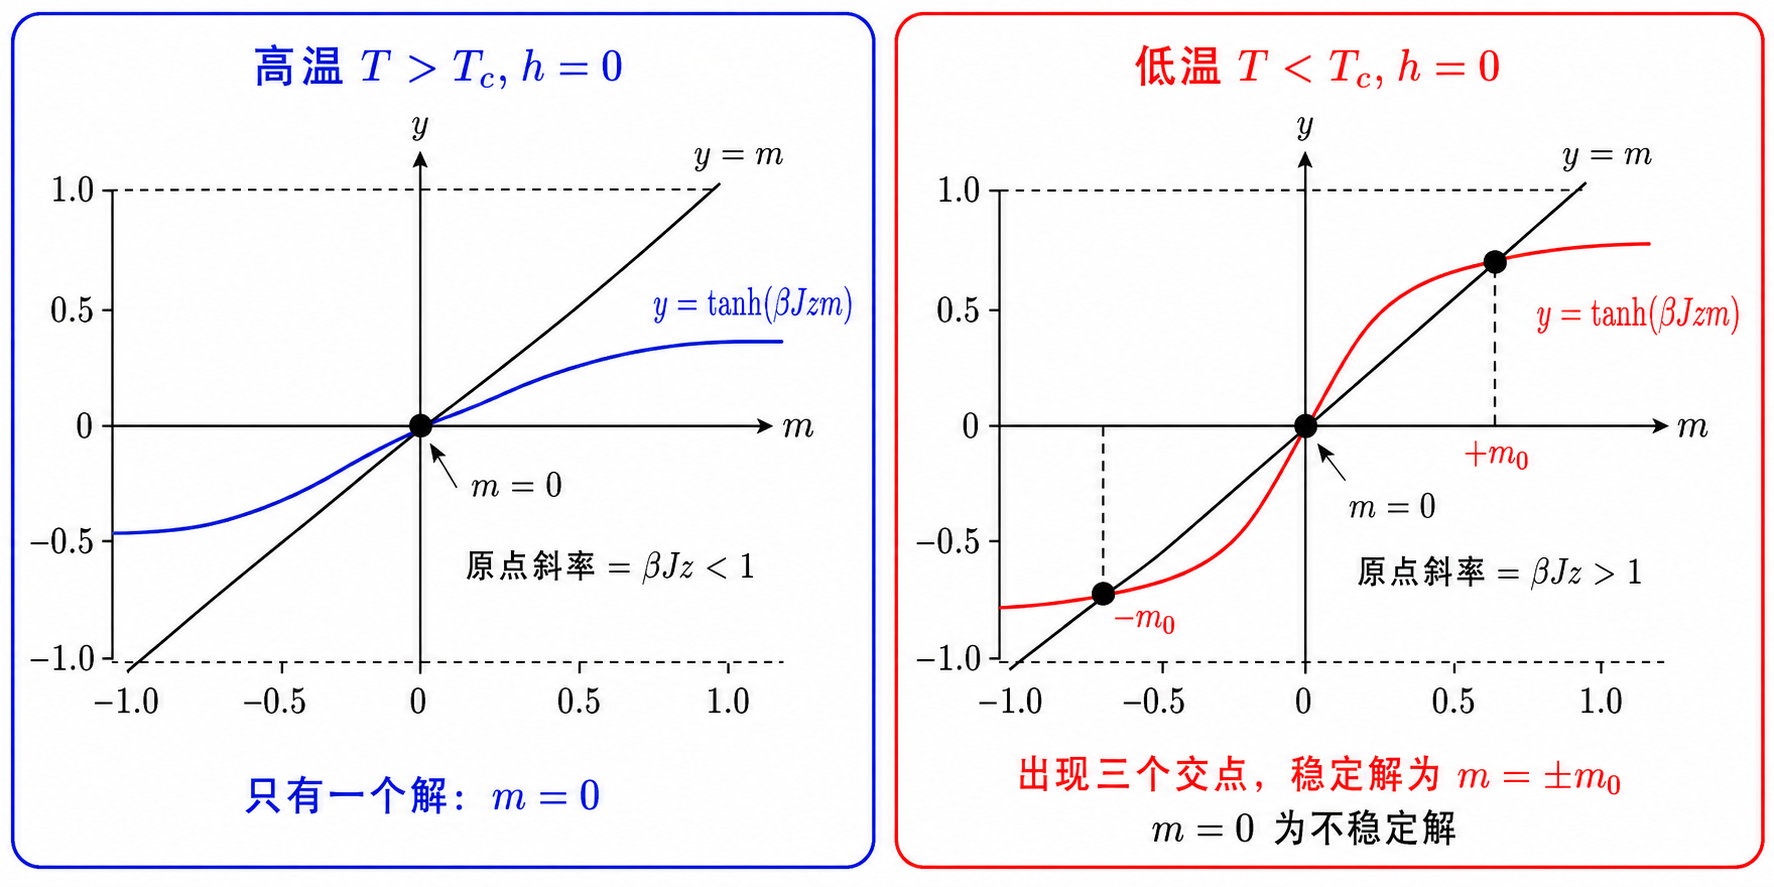
\includegraphics[width=0.6\textwidth]{fig/statistical_mechanics/MFT_scfeq.png}
\end{figure}

判断相变的方法：\textcolor{blue}{\textbf{从斜率0(相当于$T=0 \ \rm K$)开始旋转$y=m$，这意味着改变温度，如果与$\tanh(\beta(h+Jmz))$的交点从非0变成0了，就说明发生了相变。一阶相变则是直接从非0跳到0了。二阶相变是连续地到0。}}

通过自洽方程求解临界温度既可以画图解，也可以用 Taylor 展开分析。令$h=0$，$m\to0$，自洽方程变成：
\[m=\tanh(\beta zJm)=\beta zJm-\frac{(\beta zJm)^3}{3}+\cdots \quad \Rightarrow \quad 1=\eval{\dv{m}{m}}_{h,m=0}=\eval{\dv{}{m}\tanh(\beta zJm)}_{h,m=0}\quad\Rightarrow\quad \beta_c zJ=1\]

平均场近似给出的$T_c$不是精确值，例如一维 Ising 模型精确结果是$T_c=0$，而平均场会错误给出$T_c=2J/k_{\rm B}$；这正是因为一维涨落太强，平均场忽略涨落后会过度乐观地预测有序。这个结论可以用一个非常简单的 domain wall 论证看出来。考虑一维铁磁 Ising 链，在$T=0$时基态为全体自旋同向$\uparrow\uparrow\uparrow\cdots\uparrow$或$\downarrow\downarrow\downarrow\cdots\downarrow$。对开放链，基态能量为$E_0=-(N-1)J$，熵为$S=0$。现在在链中制造一个 domain wall，如$\uparrow\uparrow\uparrow\downarrow\downarrow\downarrow$只有跨过 domain wall 的那一条键从同向变成反向，能量由$-J$变成$+J$，所以能量代价为$\Delta E=2J$。这个 domain wall 可以放在大约$N-1$个不同的位置，因此带来构型熵：
\[\Delta S = k_{\rm B}\ln (N-1) \simeq k_{\rm B}\ln N \quad \Rightarrow \quad \Delta F=\Delta E-T\Delta S\simeq 2J-k_{\rm B}T\ln N\]
只要$T>0$，在热力学极限$N\to\infty$下都有$\Delta F\to-\infty$，也就是说 domain wall 的增殖会降低自由能。大量 domain wall 会把长程有序切成许多有限畴，最终使平均磁化强度消失。因此一维短程 Ising 模型没有有限温度铁磁相变，精确地说$T_c=0$。这个例子也说明了平均场为什么会失败：它只看到一个自旋周围的平均环境，却看不到低维体系中这种代价有限、熵收益随系统大小增长的畴壁涨落。

上述结论实际上是 Ising 模型的精确结论，考虑一维周期链$s_{N+1}=s_1$：
\[H=-J\sum_{i=1}^{N}s_is_{i+1}-h\sum_{i=1}^{N}s_i \quad \Rightarrow \quad Z=\sum_{s_1,\cdots,s_N=\pm1}\prod_{i=1}^{N}\exp\left[\beta Js_is_{i+1}+\frac{\beta h}{2}(s_i+s_{i+1})\right]\]
于是定义 transfer matrix：
\[\mel{s}{T}{s'}=\exp\left[\beta Jss'+\frac{\beta h}{2}(s+s')\right] \quad \Rightarrow \quad T=\begin{pmatrix}
e^{\beta(J+h)} & e^{-\beta J}\\
e^{-\beta J} & e^{\beta(J-h)}
\end{pmatrix}\]
配分函数就变成矩阵迹，可以用本征值表示：
\[Z=\Tr T^N=\lambda_+^N+\lambda_-^N, \quad \lambda_\pm=e^{\beta J}\left[\cosh(\beta h)\pm\sqrt{\sinh^2(\beta h)+e^{-4\beta J}}\right]\]
由$\lambda_+>\lambda_-$可知在热力学极限$N \to \infty$下只需要考虑$\lambda_+$的贡献，所以单位自由能$f$和单位磁化强度$m$为：
\[f=-\frac{1}{\beta N}\ln Z=-\frac{1}{\beta}\ln\lambda_+, \quad m=-\pdv{f}{h}=\frac{\sinh(\beta h)}{\sqrt{\sinh^2(\beta h)+e^{-4\beta J}}}\]
因此只要$T>0$，令$h\to0$都有$m=0$。只有在$T=0$时，$e^{-4\beta J}\to0$，体系才会非解析地选择$m=\pm1$。这说明一维短程 Ising 模型的精确临界温度确实为$T_c=0$。这个结论依赖相互作用是短程的，若一维相互作用足够长程，例如$J_{ij}$随距离衰减得很慢，domain wall 的能量代价不再只是常数，一维系统也可能出现有限温度相变。

\begin{figure}[htbp]
\centering
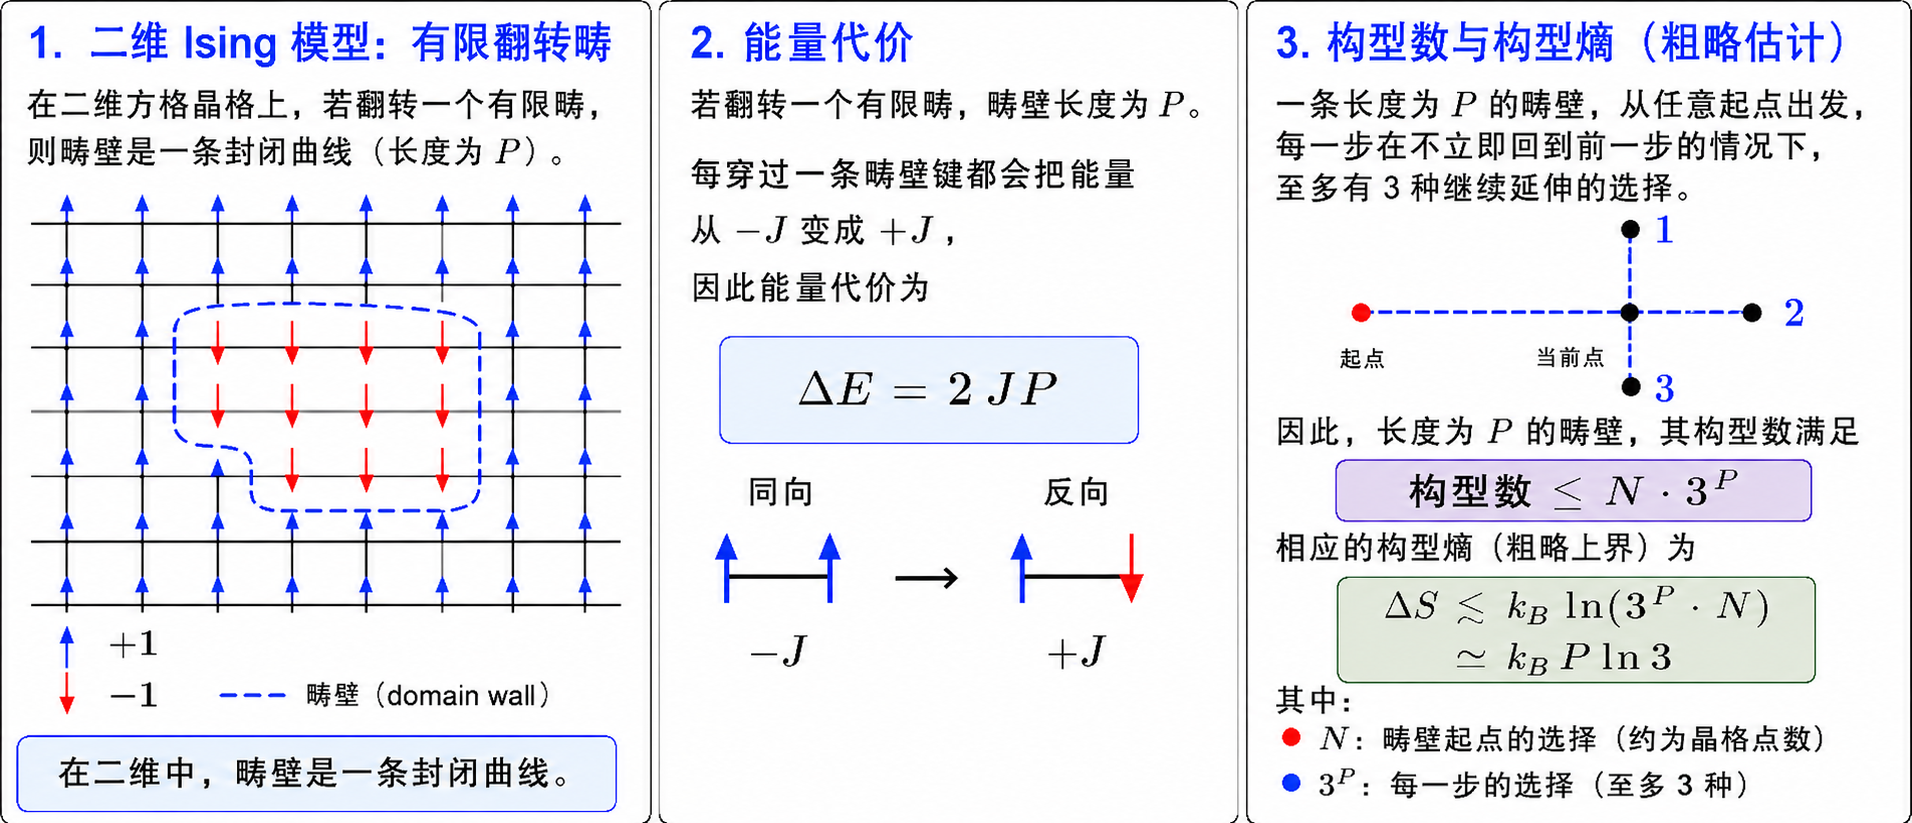
\includegraphics[width=0.8\textwidth]{fig/statistical_mechanics/2dising.png}
\end{figure}

二维 Ising 模型的情况不同。此时 domain wall 不再是一个点，而是一条闭合曲线。若翻转一个有限畴，畴壁长度为$P$，每穿过一条畴壁键都会把能量从$-J$变成$+J$，所以能量代价为$\Delta E=2JP$，粗略估计一条长度为$P$的畴壁每一步至多有$3$种继续延伸的选择，因此可能畴壁数目不超过$3^P$，对应构型熵变为和自由能变为：
\[\Delta S\lesssim k_{\rm B}\ln(3^P\cdot N)\simeq k_{\rm B}P\ln3 \quad \Rightarrow \quad \Delta F\gtrsim P(2J-k_{\rm B}T\ln3)\]
当$T<2J/(k_{\rm B}\ln3)$时自由能代价随周长$P$线性增加，所以低温铁磁长程序稳定。这就是 Peierls argument 的核心。它不能给出精确$T_c$，但是它证明了二维短程 Ising 模型确实存在有限温度有序相。二维 Ising 模型的精确解由 \href{https://theory.tifr.res.in/~tridib/ReferenceMaterial/PlischkeBergersen_Sec.6.1.pdf}{Onsager} 给出，讲义中介绍的思路仍然是 transfer matrix，只是矩阵从一维的$2\times2$矩阵变成了按整行自旋构型标记的大矩阵。

考虑周期性边界条件下的$N\times N$的二维方格 Ising 模型，并先取$h=0$：
\[H=-J\sum_{i,j}\left(s_{i,j}s_{i+1,j}+s_{i,j}s_{i,j+1}\right)\]
这里第一项可以看成相邻两行之间的相互作用，第二项可以看成同一行内部的相互作用。定义第$j$行的整行自旋构型为$\mu_j=\{s_{1,j},s_{2,j},\cdots,s_{N,j}\}$，则可定义 transfer matrix，其矩阵元为：
\[\mel{\mu_j}{T}{\mu_{j+1}}=\exp\left[\beta J\sum_{i=1}^{N}s_{i,j}s_{i,j+1}+\beta J\sum_{i=1}^{N}s_{i,j}s_{i+1,j}\right]\]
这样配分函数仍然可以写成矩阵迹：
\[Z=\sum_{\mu_1,\cdots,\mu_N}\mel{\mu_1}{T}{\mu_2}\mel{\mu_2}{T}{\mu_3}\cdots\mel{\mu_N}{T}{\mu_1}=\Tr T^N\]
形式上这和一维完全一样，只是$T$现在是$2^N\times2^N$矩阵。若$\lambda_{\max}$是最大本征值，则热力学极限中：
\[Z\simeq \lambda_{\max}^{N},\quad f=-\frac{k_{\rm B}T}{N^2}\ln Z\simeq-\frac{k_{\rm B}T}{N}\ln\lambda_{\max}\]
Onsager 的工作本质上就是在$N\to\infty$极限中求出这个最大本征值。最终零场自由能密度可以写成：
\[f=-k_{\rm B}T\ln\left[2\cosh(2\beta J)\right]-\frac{k_{\rm B}T}{2\pi}\int_0^\pi\ln\left[\frac{1+\sqrt{1-\kappa^2\sin^2\phi}}{2}\right]\dd{\phi}, \quad \kappa=\frac{2\sinh(2\beta J)}{\cosh^2(2\beta J)}\]
这个表达式的非解析性来自积分中的平方根。当$\kappa<1$时被积函数光滑；临界点出现在$\kappa=1$，也就是：
\[\frac{2\sinh(2\beta_cJ)}{\cosh^2(2\beta_cJ)}=1 \quad \Leftrightarrow \quad \sinh(2\beta_cJ)=1 \quad \Rightarrow \quad k_{\rm B}T_c=\frac{2J}{\ln(1+\sqrt2)}\simeq2.269J\]
这个值低于平均场估计$k_{\rm B}T_c=zJ=4J$，说明二维涨落虽然没有强到完全消灭相变，但已经显著降低了临界温度。自由能公式还可以给出热容奇异性。热容可以由自由能的二阶导数获得：
\[C=-T\pdv[2]{f}{T}\sim -\ln\left|1-\frac{T}{T_c}\right|\]
当温度$T$趋于$T_{\rm c}$时，热容对数发散，说明二维 Ising 模型的热容指数$\alpha=0$。回到平均场理论，平均场不仅能估计$T_c$，还可以给出一整套临界指数。从自洽方程$m=\tanh\beta(h+Jmz)$，在零外场$h=0$下定义约化温度$t=(T-T_c)/T_c$。在$T$接近$T_c$时，$\beta zJ=T_c/T\simeq1-t$，展开到三阶项$m^3$：
\[m=(1-t)m-\frac{1}{3}(1-t)^3m^3 \simeq (1-t)m-\frac{1}{3}m^3 \quad \Leftrightarrow \quad tm+\frac{1}{3}m^3=0\]
当$T>T_c$时$t>0$，只有$m=0$；当$T<T_c$时$t<0$，非零解为：
\[m^2\simeq-3t,\quad m\propto(-t)^{1/2}\]
所以平均场给出临界指数$\beta_{\rm MF}=1/2$。磁化率$\chi$可以直接对自洽方程求导获得：
\[\chi=\eval{\pdv{h}\tanh\beta(h+Jmz)}_{h,m=0}\simeq\beta\eval{\pdv{h}(h+Jmz)}_{h,m=0}=\beta(1+zJ\chi) \quad \Leftrightarrow \quad \chi=\frac{\beta}{1-\beta zJ}\propto\frac{1}{T-T_c}\]
因此平均场给出$\gamma_{\rm MF}=1$。取$T=T_c$并保留小$m$和小$h$，则：
\[m=\tanh\beta(Jmz+h)\simeq \beta Jmz+h-\frac{1}{3}(\beta Jmz+h)^3\simeq m+h-\frac{1}{3}(\beta Jmz+h)^3 \quad \Rightarrow \quad h\simeq\frac{1}{3}m^3\]
因此：
\[m\propto h^{1/3},\quad \delta_{\rm MF}=3\]
上述平均场结论依然满足 Rushbrooke 标度关系$\alpha+2\beta+\gamma=2$。

\newpage
\subsection{一维 Landau 平均场理论和 Ginzburg 判据}
另一条近似 Ising 模型的路是 Landau 平均场理论。它不从具体显微 Hamiltonian 出发，而是根据对称性写自由能。零外场 Ising 模型在$m\to -m$下不变，因此自由能只能含$m$的偶次幂；外场$h$会线性耦合到$m$：
\[f_{\rm L}(m)=f_0+\frac{r}{2}m^2+\frac{u}{4!}m^4-hm+\cdots,\quad u>0\]
上述幂函数的系数可以从平均场的自由能（忽略对数前的系数）获得：
\[f_{\rm MF}(m)=-k_{\rm B}T\ln\left[2\cosh\beta(h+Jmz)\right]\simeq-k_{\rm B}T\left[\ln2+\frac{1}{2}\beta^2(h+Jmz)^2-\frac{1}{12}\beta^4(h+Jmz)^4+\mathcal{O}(\beta^6)\right]\]
容易解出：
\[f_0=-k_{\rm B}T\ln2, \quad r=\frac{zJ}{2}(k_{\rm B}T-zJ)\approx k_{\rm B}(T-T_c), \quad u=2zJ\approx2k_{\rm B}T\]
平衡条件为：
\[\pdv{f_{\rm L}}{m}=rm+\frac{u}{6}m^3-h=0\]
当$h=0$且$r>0$时，唯一极小值为$m=0$；当$r<0$时，$m=0$变为极大值，出现两个等价极小值：
\[m_0^2=-\frac{6r}{u}\propto T_c-T\]
因此再次得到$\beta_{\rm MF}=1/2$。当$T>T_c$且$h$很小时，$m\simeq h/r$，所以$\chi\simeq1/r\propto(T-T_c)^{-1}$，即$\gamma_{\rm MF}=1$。当$T=T_c$时$r=0$，有$h=(u/6)m^3$，所以$\delta_{\rm MF}=3$。热容指数也可以从 Landau 自由能读出。对$T>T_c$，极小值在$m=0$，奇异部分$f_{\rm sing}=0$；对$T<T_c$，代入$m_0^2=-6r/u$：
\[f_{\rm sing}=\frac{r}{2}m_0^2+\frac{u}{4!}m_0^4=-\frac{3r^2}{2u}\propto-(T-T_c)^2\]
热容为：
\[C=-T\pdv[2]{f}{T}\]
所以在$T_c$处只有有限跳变，没有幂律发散，故$\alpha_{\rm MF}=0$。综上所述，平均场的临界指数整理为：
\[\alpha_{\rm MF}=0,\quad \beta_{\rm MF}=\frac{1}{2},\quad \gamma_{\rm MF}=1,\quad \delta_{\rm MF}=3\]
它们满足 Rushbrooke 标度关系$\alpha+2\beta+\gamma=2$。

最后的一个问题：平均场什么时候可靠？这正是\href{https://en.wikipedia.org/wiki/Ginzburg_criterion}{Ginzburg 判据}回答的问题。平均场假设在一个相关体积$\xi^d$内，序参量涨落远小于平均值本身：
\[\expval{(\delta m)^2}_{\xi}\ll m^2\]
由涨落-耗散关系，相关体积内的涨落量级可以估计为：
\[\int_0^\xi\left(\expval{s_rs_0}-\expval{s_r}\expval{s_0}\right)\dd[d]{r}=k_{\rm B}T\chi\]
而平均场给出：
\[m^2\propto |t|,\quad \chi\propto |t|^{-1},\quad \xi\propto |t|^{-1/2}\]
于是相对涨落量级为：
\[\frac{k_{\rm B}T\chi}{m^2\xi^d}\propto\frac{|t|^{-1}}{|t|\cdot |t|^{-d/2}}=|t|^{\frac{d-4}{2}}\]
若$d>4$，当$t\to0$时这个比值趋于$0$，平均场在临界点附近自洽；若$d<4$，这个比值发散，越接近临界点涨落越压倒平均值，平均场失效。因此 Ising 型短程相互作用体系的上临界维数为$d_c=4$。

这给了一个非常实用的判断方法：如果只需要求最坏情况下估计性质，可以先做平均场，得到$T_c$的数量级、自由能形状、序参量行为和临界指数；但如果需要处理低维、短程相互作用或临界区，就必须警惕涨落修正。相互作用范围越长，或者实验可达的临界区越窄，平均场越可能在较宽温度范围内看起来有效；而对于低维短程体系，真正靠近$T_c$时通常会出现非平均场行为。
